\documentclass[a4paper]{book}

%pachete folosite
\usepackage{graphicx}
\usepackage{fullpage}
\usepackage{verbatim}
\usepackage{url}
%pachete folosite

%calea catre diagrame
\graphicspath{{diagrame/}}
%calea catre diagrame

%pentru diacritice
\newcommand{\myqq}{''}
\catcode`\'=13
\newcommand{'}[1]{\ifmmode {}^\prime \noexpand#1%
\else\ifx#1a\u{a}% 
\else\ifx#1i\^{i}%
\else\ifx#1s\c{s}% 
\else\ifx#1t\c{t}%
\else\ifx#1j\^{a}%
\else\ifx#1A\u{A}% 
\else\ifx#1I\^{I}%
\else\ifx#1S\c{S}% 
\else\ifx#1T\c{T}%
\else\ifx#1J\^{A}%
\else\ifx#1'\myqq%
	\fi\fi\fi\fi\fi\fi\fi\fi\fi\fi\fi%
\fi}
%pentru diacritice

%titluri in romana 
\def\contentsname{Cuprins}
\renewcommand{\figurename}{Figura}
\renewcommand{\tablename}{Tabelul}
\renewcommand{\chaptername}{Capitolul}
\renewcommand{\bibname}{Bibliografie}
%titluri in romana


%DOCUMENTUL PROPRIU-ZIS
\begin{document}

%pagina de titlu

%linie orizontala
\newcommand{\HRule}{\rule{\linewidth}{0.5mm}}
%linie orizontala

%data in format romanesc
\def\today{\space  \ifcase \month
\or IANUARIE\or FEBRUARIE\or mARTIE\or APRILIE\or MAI\or IUNIE\or
IULIE\or AUGUST\or SEPTEMBRIE\or OCTOMBRIE\or NOIEMBRIE\or DECEMBRIE \fi
\space  \number\year}
%data in format romanesc

%pagina de titlu
\begin{titlepage}
\begin{center}
  
%facultatea
\textsc{\LARGE Universitatea Bucure'sti}\\
\textsc{\LARGE Facultatea de matematic'a 'si informatic'a}\\[1.0cm]
%facultatea
 

\textsc{\Large Lucrare de licen't'a}\\[3.0cm]
 
 
%Titlu
\HRule \\[0.5cm]
{ \huge \bfseries Securitatea pe Internet}\\[0.4cm]
\HRule \\[4.5cm]
%Titlu
 
%autor si coordonator
\begin{minipage}{0.4\textwidth}
\begin{flushleft} \large
\emph{Autor:}\\
C'alin \textsc{Avas'ilc'ai}
\end{flushleft}
\end{minipage}
\begin{minipage}{0.4\textwidth}
\begin{flushright} \large
\emph{Coordonator:} \\
Prof. Dr. Adrian \textsc{Atanasiu}
\end{flushright}
\end{minipage}
%autor si coordonator
 
\vfill
 
%data curenta
{\large \today}
%data curenta
 
\end{center}
\end{titlepage}
%pagina de titlu
%pagina de titlu

%cuprins
\tableofcontents
%cuprins

%CapI introducere
\chapter{Introducere}

Securitatea este un domeniu cuprinz'ator, care acoper'a o multitudine de aspecte. Securitatea informa'tiei presupune protejarea informa'tiei 'si sistemelor prin care aceasta circul'a de acces, folosire, divulgare sau modificare neautorizat'a ori distrugere. O ramur'a a acestui domeniu este reprezentat'a de securitatea pe Internet. 

Re'teaua pe care noi o numim ast'azi Internet a fost construit'a ca o re'tea militar'a 'si, ca urmare, a fost proiectat'a pentru a rezista p'jn'a 'si unui atac nuclear. De'si Internetul nu a fost testat 'in condi'tii at'jt de dramatice, putem 'ins'a afirma c'a arhitectura sa se ridic'a la 'inaltimea a'stept'arilor. 

Proiectan'tii nu au conceput 'ins'a re'teaua pentru a rezista unui alt tip de atac: din interior. Acum, c'jnd re'teaua s-a 'intins la dimensiuni neimaginate, aceast'a lips'a se dovede'ste foarte grav'a.

Internetul nu este o singur'a re'tea, ci o colec'tie la nivel global de re'tele interconectate, ce poate fi accesat'a de un calculator 'intr-o multitudine de feluri: gateway-uri, router-e, conexiuni dial-up, provideri de servicii Internet(ISP). Internetul este u'sor de accesat pentru oricine are un calculator conecat la o re'tea. Indivizi 'si organiza'tii din toat'a lumea pot accesa orice punct din re'tea indiferent de pozi'tia geografic'a.

Dar, pe l'jng'a aceste uria'se avantaje, exist'a 'si riscuri. Informa'tia este expus'a pericolelor precum pierderea, furtul sau coruperea. Dac'a informa'tia este stocat'a intr-un mediu electronic 'si acest mediu este cuplat la re'tea, aceast'a informa'tie este mai vulnerabil'a dec'jt dac'a ar fi fost scris'a pe o bucat'a de h'jrtie 'si inchis'a intr-un cabinet. Intru'sii nu trebuie s'a intre 'intr-un birou sau o cas'a, nici m'acar nu trebuie s'a fie 'in aceea'si 'tar'a. Pot fura sau copromite informa'tie f'ar'a s'a ating'a vreo bucat'a de h'jrtie. Mai mult, 'i'si pot rula propriile programe 'si pot ascunde dovezile activit'a'tii neautorizate.

Dimensiunea uria's'a a re'telei, num'arul enorm de calculatoare cuplate, existen'ta a zeci de bug-uri 'in implement'arile programelor care se execut'a pe aceste calculatoare, 'si inten'tiile du'sm'anoase a c'jtorva in'si formeaza un cocteil exploziv. Situa'tia se 'inr'aut'a'te'ste pe zi ce trece, 'si cracker-ii sunt 'intr-o curs'a continu'a cu proiectan'tii re'telei 'si cu administratorii de sistem, care 'incearc'a s'a remedieze defec'tiunile acesteia. Din p'acate, acesta este un razboi la al c'arui 'inceput abia asist'am, 'si care nu are un sf'jr'sit previzibil 'in viitorul apropiat.

Principala problem'a este constituit'a de faptul c'a o mare parte din protocoalele ce alc'atuiesc suita TCP/IP care st'a la baza Internetului au fost proiectate c'jnd aceast'a re'tea nu era dec'jt un mic grup de sisteme informatice controlate de persoane care se cuno'steau 'intre ele, 'si care aveau 'incredere unele 'in altele sau, cel pu'tin, puteau folosi mijloace ``fizice'' de securitate. Proiectan'tii nu 'si-au imaginat niciodat'a c'a TCP/IP va ajunge s'a fie folosit de milioane de oameni din toat'a lumea 'si c'a va avea nevoie de mecanisme de securitate mult mai complexe dec'jt ar fi avut nevoie pe vremea aceea. De aceea au neglijat problema securit'a'tii, iar dup'a ce aceste protocoale s-au standardizat 'si au 'inceput s'a fie folosite la nivel global a fost prea t'jrziu pentru o reproiectare.

'In aceast'a lucrare voi discuta mai 'int'ji despre sl'abiciunile arhitecturii Internetului; sl'abiciuni ce pot fi exploatate de anumi'ti indivizi cu diverse scopuri. Voi trece apoi la a clasifica tipurile de atacuri ce pot avea loc pe Internet 'si voi analiza c'jteva dintre acestea. 'In final voi trata subiectul unuia dintre mecanismele ce pot fi folosite pentru a dejuca planurile unor eventuali atacatori: ``zidurile de foc'' sau firewall-urile.

%CapII Slabiciunile protocoalelor TCP/IP
\chapter{Sl'abiciunile protocoalelor TCP/IP}

%CapII 1 Protocoalele de baza
\section{Protocoalele de baz'a}

Sintagma TCP/IP este o prescurtare pentru o colec'tie de protocoale de comunicare. A fost proiectat'a sub auspiciile DARPA
(U.S Defense Advanced Ressearch Projects Agency) 'si folosit'a la vechiul ARPANET, precursorul a ceea ce numim ast'azi Internet, 
'in 1983.

O schem'a a fluxului de date este reprezentat'a in Figura \ref{diferitenivele}. Fiecare nivel reprezint'a un protocol din suita de protocoale TCP/IP.
Nivelul superior con'tine aplica'tiile: mail, login, etc. Aplica'tiile folosesc componentele nivelelor inferioare pentru a transmite 
'si a recep'tiona date. 'In mijlocul ``p'jnzei de p'aianjen'' gasim protocolul numit IP(Internet Protocol). IP este un multiplexor de pachete.
Mesajelor de la protocoale de nivel mai 'inalt li se ata'seaz'a un antet IP 'si apoi sunt trimise la interfa'ta cu re'teaua pentru a fi transmise
mai departe.

\begin{figure}[ht]
	\centering
	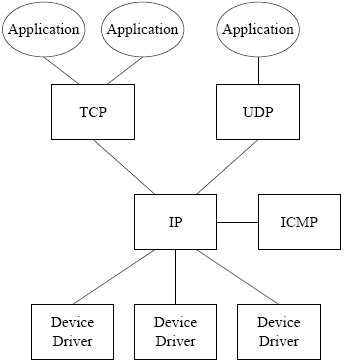
\includegraphics[scale=.7]{tcp_ip_layering.jpg}
	\caption{Diferitele nivele care apar 'in TCP/IP}
	\label{diferitenivele}
\end{figure}

S'a examin'am protocolul IP.
%2.1.1 IP
\subsection{IP}
Despre pachetele IP se poate spune c'a stau la baza suitei de protocoale TCP/IP. Fiecare pachet con'tine adresa nodului surs'a 'si 
adresa nodului destina'tie, pe c'jte 32 de bi'ti, c'j'tiva bi'ti de op'tiuni, un \emph{cecksum}(sum'a a octe'tilor) al antetului 'si datele propriu-zise. Un pachet IP obi'snuit are c'jteva sute de octe'ti. Astfel de pachete c'al'atoresc cu miliardele 'in lumea diferitelor tipuri de re'tele cum ar fi Ethernet, FDDI rings(Fiber Distributed Data Interface), serial lines, ATM(Asynchronous Transfer Mode), re'tele wireless, etc.

Nu exist'a conceptul de circuit virtual sau conexiune la nivelul IP, cu alte cuvinte, fiecare pachet este de sine st'at'ator. IP este un protocol nedemn de 'incredere deoarece nu exist'a nici o garan'tie c'a pachetele vor ajunge la destina'tie, c'a vor ajunge la destina'tie o singur'a dat'a sau c'a vor ajunge 'in ordinea 'in care au fost trimise. Nici m'acar nu se verific'a corectitudinea; checksum-ul din antet acoper'a numai antetul. De fapt, nu exist'a nici o garan'tie c'a pachetul chiar a fost trimis de un calculator cu adresa IP men'tionat'a 'in antet. De'si sistemele de operare se asigur'a c'a pachetele pleac'a cu un antet corect, nu ne putem baza pe validitatea adresei surs'a 'inscrise 'in pachet, dec'jt 'in anumite circumstan'te. Pentru autentificare 'si securitate 'in general trebuiesc implementate mecanisme 'in nivelele superioare. Un pachet care calatore'ste o distan't'a lung'a va trece prin multe noduri intermediare p'jn'a ce va ajunge la destina'tie. O conexiune direct'a 'intre dou'a noduri consecutive care fac parte din ruta aleas'a pentru un pachet se nume'ste ``hop''. Fiecare hop are cap'at final o gazd'a sau un router, ultimul 'inaint'and pachetul spre urmatorul hop, pe baza informa'tiei de rutare. 'In timpul acestor opera'tiuni pachetul 'in cauz'a poate fi fragmentat 'in buc'a'ti mai mici dac'a este prea mare pentru un anumit hop(unele tipuri de re'tele au o limit'a mai mic'a dec'jt altele 'in ceea ce prive'ste dimensiunea fragmentelor de date ce pot fi puse pe fir la un momentdat). Un router poate renun'ta la unele pachete dac'a este prea aglomerat. Pachetele pot sosi la destina'tie 'intr-o ordine diferit'a de cea 'in care au fost trimise, sau chiar duplicate. Protocoale de nivel superior(TCP) trebuie s'a se ocupe de aceste probleme 'si s'a asigure un circuit fiabil pentru aplica'tie.

Dac'a un pachet este prea mare pentru urm'atorul hop va fi fragmentat, adic'a va fi 'impar'tit 'in dou'a sau mai multe pachete, fiecare cu antetul s'au 'si doar o parte din datele propriu-zise. Fragmentele vor c'al'atori individual p'jn'a la destina'tie, posibil pe alte rute. 'In timpul c'al'atoriei aceste fragmente pot fi iar'a'si fragmentate. C'jnd buc'a'tile ajung la calculatorul destina'tie, ele sunt reasamblate. Nu se fac reasambl'ari la hopuri intermediare.

\begin{figure}[ht]
	\centering
	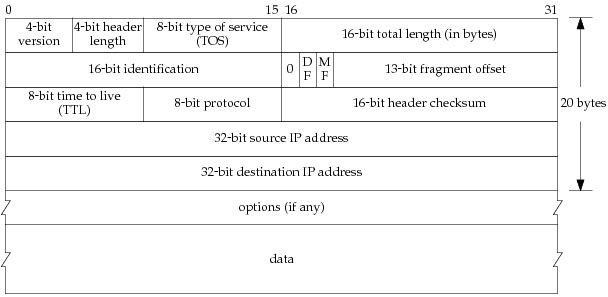
\includegraphics[scale=.7]{ip_header.jpg}
	\caption{Structura unui pachet IP}
	\label{antetip}
\end{figure}

\subsubsection{Adresele IP}
Adresele 'in IP versiunea 4(IPv4, 'inc'a cea mai r'asp'jndit'a) sunt reprezentate pe 32 de bi'ti 'si sunt 'imp'ar'tite 'in dou'a por'tiuni: o por'tiune de re'tea 'si o por'tiune de gazd'a. Limit'a 'intre cele dou'a este setat'a de administratorul re'telei 'si poate varia. Vechea no'tiune de limite fixe 'intre cele dou'a por'tiuni a fost 'inlocuit'a de o alt'a abordare numit'a \emph{CIDR}(Classless Inter-Domain Routing). O adres'a IP scris'a sub forma CIDR arat'a 'in felul urm'ator: 207.99.106.123/23. 'In acest exemplu primii 23 de bi'ti reprezint'a por'tiunea de re'tea iar restul por'tiunea gazd'a. Por'tiunile gazd'a cu to'ti bi'tii 0 sau 1 sunt rezervate pentru opera'tiuni broadcast. 

\subsubsection{Etichetele de securitate IP}
IP are c'jteva c'jmpuri op'tionale care nu sunt folosite frecvent. 'In contextul securit'a'tii cele mai importante sunt eticheta de securitate 'si rutarea de tip ``strict source routing'' sau ``loose source routing''.

Op'tiunea ``IP security'' e folosit'a de obicei de site-urile militare. Fiecare pachet este etichetat cu tipul de informa'tie pe care o con'tine. Eticheta include at'jt o component'a ierarhic'a(Secret, Top Secret, etc.) c'jt 'si o categorie op'tional'a: arme nucleare, criptografie, etc. Eticheta indic'a nivelul de securitate al ultimului nod care a primit pachetul. Este posibil ca un router s'a nu trimit'a pachetul printr-un mediu cu un nivel de securitate mai sc'azut dec'jt cel men'tionat de pachet deoarece acest fapt ar putea conduce la aflarea informa'tiei confiden'tiale. Din motive evidente, s-ar putea s'a nu citeasc'a dintr-un mediu care con'tine informa'tie secret'a. Combina'tia celor dou'a restric'tii va for'ta de obicei cele dou'a procese de la capetele conexiunii s'a aib'a acela'si nivel de securitate. Unele sisteme, cum ar fi Unix V/MLS, p'astreaz'a c'jte o etichet'a de securitate pentru fiecare proces. Prin urmare se poate ata'sa eticheta de securitate cuvenit'a fiec'arui pachet 'in func'tie de procesul care 'il trimite. Pentru calculatoare conven'tionale router-ul poate ata'sa pentru fiecare pachet primit pe o anumita interfa't'a o anumit'a op'tiune de securitate. Principalul scop al etichetelor de securitate este de a constr'jnge deciziile de rutare. Un pachet marcat ``Top Secret'' nu va fi rutat pe o leg'atur'a care nu este sigur'a dec'jt pentru trafic normal.
%2.1.1 IP

%2.1.2 ARP
\subsection{ARP}
Pachetele IP circul'a de obicei prin re'tele Ethernet. Dispozitivele Ethernet ``nu in'teleg'' adresele IP pe 32 de bi'ti, ci transmit pachete Ethernet ce con'tin adrese pe 48 de bi'ti. Ca urmare, un driver IP va trebui s'a traduc'a o adres'a IP destina'tie 'intr-o adres'a Ethernet. De'si exist'a unele coresponden'te statice sau algoritmice 'intre cele dou'a tipuri de adrese, de obicei este nevoie de un tabel care s'a stocheze coresponden'tele. Protocolul ARP(Address Resolution Protocol) este folosit pentru a determina aceste map'ari. 

ARP func'tioneaz'a 'in felul urm'ator: trimite un pachet Ethernet de tip broadcast care con'tine adresa IP pentru care se dore'ste s'a se afle coresponden'ta; gazda care are acea adres'a(sau un sistem care se d'a drept acea gazd'a) r'aspunde cu un pachet care con'tine coresponden'ta dorit'a(adresa IP, adresa Ethernet); coresponden'ta este stocat'a apoi 'in memorie pentru a reduce traficul.

Exist'a un pericol aici dac'a toate nodurile au drept de scriere 'in re'teaua local'a. Un nod ar putea s'a emita mesaje ARP false 'si s'a devieze tot traficul spre el 'insu'si; poate pretinde c'a este nodul destina'tie sau poate modifica datele en passant.

Mecanismul ARP este de obicei automat. 'In re'tele speciale cu securitate ridicat'a, map'arile ARP pot fi statice.
%2.1.2 ARP

%2.1.3 TCP
\subsection{TCP}
TCP(Transmission Control Protocol) asigur'a un circuit virtual(conexiune) fiabil pentru procesele ce ruleaz'a pe o gazd'a. Pachetele pierdute sau avariate sunt retransmise; pachetele primite sunt reordonate dac'a este necesar. Ordonarea este men'tinut'a de numere de ordine atribuite fiec'arui pachet. Fiecare octet timis, c'jt 'si cererile de creere/'inchidere conexiune sunt numerotate individual. Toate pachetele 'in afar'a de primul pachet trimis 'in contextul unei conexiuni con'tin 'si un num'ar de confirmare(ACK) a'sa cum se poate remarca 'in Figura \ref{conexiunetcp}; acest num'ar reprezint'a num'arul de ordine al ultimului octet recep'tionat cu succes.

\begin{figure}[ht]
	\centering
	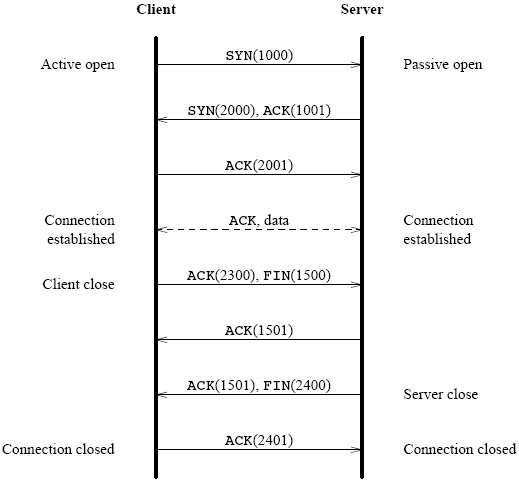
\includegraphics[scale=.7]{tcp_connection_flow.jpg}
	\caption{Desf'a'surarea unei comunic'ari la nivelul TCP}
	\label{conexiunetcp}
\end{figure}

Fiecare mesaj TCP este marcat ca fiind de la o anumit'a gazd'a 'si un anumit port la o gazd'a destina'tie 'si port destina'tie. Cvadruplul $<$gazd'asurs'a, portsurs'a, gazd'adestina'tie, portdestina'tie$>$ identific'a 'in mod unic un circuit. Se 'intampl'a destul de des s'a existe mai multe circuite diferite cu acela'si port local, totul este 'in ordine at'jt timp c'jt cel pu'tin una din celelalte dou'a componente difer'a.

Serverele -- procese care asigur'a unele sevicii prin intermediul TCP -- ``ascult'a'' pe anumite porturi. Prin conven'tie, numerele porturilor serverelor sunt mici. Neonorarea acestei conven'tii poate cauza probleme de securitate. Se presupune c'a numerele porturilor pentru serviciile standard asigurate de un server sunt cunoscute de eventualii clien'ti. Un port pe care se ascult'a este, 'intr-un fel, ``pe jum'atate deschis''(half-open), deoarece numai adresa local'a 'si portul local sunt cunoscute('in cazul 'in care calculatorul are mai multe interfe'te la re'tea nici m'acar adresa local'a nu este cunoscut'a). C'jnd un pachet cu o cerere de conexiune ajunge la server celelalte c'jmpuri sunt completate. Dac'a este adecvat, sistemul de operare va clona ``conexiunea'' care ascult'a(in practic'a se nume'ste ``listening socket'') astfel 'incat viitoarele cereri s'a poat'a fi satisf'acute.

\begin{figure}[ht]
	\centering
	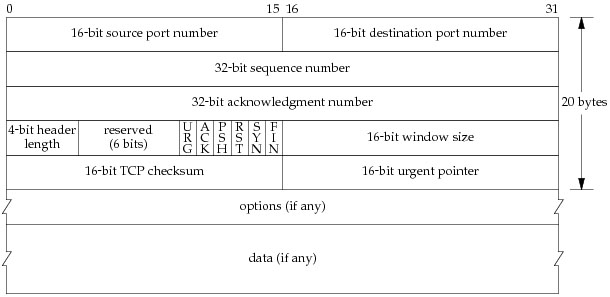
\includegraphics[scale=.7]{tcp_header.jpg}
	\caption{Structura unui pachet TCP}
	\label{antettcp}
\end{figure}

Clien'tii folosesc serviciile oferite. Procesele client rareori vor cere un anumit num'ar de port local, de'si pot face asta. 'In mod normal vor primi un oarecare num'ar de port pe care sistemul de operare 'il alege.

Multe versiuni de TCP si UDP pentru sisteme Unix nu permit dec'jt superutilizatorului(root) s'a foloseasc'a porturi mai mici dec'jt 1024. Acestea se numesc porturi privilegiate. Intentia este ca sistemul de la cel'alalt cap'at al conexiunii s'a poat'a avea 'incredere 'in autenticitatea informa'tiei scrise pe astfel de porturi. Aceast'a restric'tie e doar o conven'tie 'si nu este cerut'a in mod explicit de specifica'tia protocolului. 

Numerele de ordine men'tionate mai sus au 'si o alt'a func'tie. Deoarece num'arul de ordine ini'tial pentru noi conexiuni se schimb'a, este posibil ca TCP s'a detecteze pachete vechi de la instan'tieri precedente ale aceluia'si circuit(adic'a folosiri anterioare ale aceluia'si cvadruplu). Exist'a 'si un mic beneficiu pentru securitate: o conexiune nu poate fi stabilit'a p'jn'a ce ambele p'ar'ti nu confirm'a num'arul de ordine ini'tial al celeilalte. Acest lucru poate fi observat 'in Figura \ref{conexiunetcp} .

Exist'a un pericol ce se 'intrevede aici. Dac'a un atacator poate prezice numerele de ordine ini'tiale ale 'tintei, atunci este posibil ca atacatorul s'a p'ac'aleasc'a 'tinta f'ac'jnd-o s'a cread'a c'a vorbe'ste cu un calculator 'in care poate avea 'incredere. 'In acest caz, protocoalele care depind de adresa IP a sursei pentru autentificare(comenzile ``r'': \emph{rlogin, rsh, rexec, rcp, rwho, ruptime}) pot fi exploatate pentru a penetra sistemul 'tint'a. Un astfel de atac se nume'ste ``sequence number atack''.

Acest tip de atac depinde, 'in mare parte, de stabilirea unei conexiuni legitime cu calculatorul 'tint'a. Dac'a o astfel de conexiune este blocat'a, s'a zicem de un firewall, atacul nu va avea succes. Un dispozitiv de tip ``gateway'' care are prea mult'a ``'incredere'' 'in calculatoarele din interiorul re'telei locale poate fi vulnerabil. Conceptul de ``sequence number atack'' poate fi generalizat: alte protocoale pe l'jng'a TCP sunt vulnerabile la un astfel de atac. De fapt, a'sa-numitul ``three-way handshake'' de la stabilirea conexiunii TCP asigur'a mai mult'a protec'tie dec'jt alte protocoale.
%2.1.3 TCP

%2.1.4 SCTP
\subsection{SCTP}
Un nou protocol de transport, SCTP(\emph{Stream Control Transmission Protocol}), a fost definit recent(2000). Ca 'si TCP, asigur'a transport fiabil, dar are 'si alte c'jteva caracteristici.

Cea mai notabil'a dintre acestea este capabilitatea de a multiplexa mai multe fluxuri independete 'intr-o singur'a conexiune SCTP. Astfel, o implementare FTP, a'sezat'a peste SCTP 'in loc de TCP, nu ar avea nevoie s'a creeze o alt'a conexiune pentru transferul de date propriu-zis. Alte 'imbun'at'a'tiri includ o stabilire a conexiunii 'in patru pa'si(\emph{four-way handshake}), ceea ce 'impiedic'a atacurile distribuite(denial-of-service), marcarea 'inregistr'arilor(\emph{record-marking} - delimitarea mesajelor pentru a putea depista 'si eventual repara diferite erori) pentru fiecare flux din conexiune 'si op'tiunea de livrare neordonat'a a pachetelor(ca 'si UDP). Pentru c'a este nou, nu este suportat de majoritatea firewall-uri, adic'a nu multe firewall-uri pot filtra traficul SCTP. Mai mult, unele dintre noile 'imbun'at'a'tiri, cum ar fi capabilitatea de a ad'auga o noua adres'a IP la o conexiune 'in mod dinamic, ar putea pune probleme de securitate.
%2.1.4 SCTP

%2.1.5 UDP
\subsection{UDP}
Protocolul UDP(User Datagram Protocol) extinde acela'si nivel de servicii asigurate de IP. Livrarea pachetelor nu este asigurat'a, nu exist'a un sistem pentru corec'tie de erori, retransmisie sau detectarea pachetelor pierdute, duplicate sau amestecate. P'jn'a 'si detectarea erorilor este op'tional'a la UDP.

Lucrul care compenseaz'a pentru aceste neajunsuri este traficul sc'azut. Spre deosebire de TCP, nu exist'a conceptul de conexiune 'in contextul UDP, ceea ce 'il face potrivit pentru aplica'tii 'intrebare/r'aspuns, unde num'arul de mesaje trimise 'si recep'tionate este mic 'in compara'tie cu cel din TCP. 

C'jnd UDP este folosit pentru transmisii mari de date tinde s'a se comporte 'intr-un mod nefast 'intr-o re'tea. 'Ii lipsesc metode de control asupra fluxului de informa'tie, ceea ce poate cauza ``inundarea'' cu pachete a gazdelor sau router-elor 'si, ca urmare, pierderi mari de pachete(c'jnd un router prime'ste mai multe pachete dec'jt poate m'jnui la un momentdat, acestea sunt pierdute; opera'tia poart'a numele de ``packet drop''). 

UDP folose'ste acela'si concept de port care serve'ste la demultiplexarea unui pachet la un anumit proces 'si aceleasi conven'tii pentru servere ca 'si TCP, dar are un spa'tiu de adresare separat. 'In mod similar, serverele obi'snuiesc s'a foloseasc'a numere de porturi mici. Nu exist'a no'tiunea de circuit; toate pachetele destinate unui anumit port sunt predate aceluia'si proces indiferent de adresa IP surs'a sau portul surs'a. 

Un atac de tip ``spoof''('inlocuirea adresei surs'a 'intr-un pachet cu o adres'a fictiv'a diferit'a de adresa calculatorului responsabil de trimiterea pachetului) este mai facil asupra UDP dec'jt asupra TCP, deoarece nu exist'a ``handshake'' la stabilirea conexiunii sau numere de ordine a'sa cum se poate vedea 'si 'in antetul unui pachet UDP reprezentat 'in Figura \ref{antetudp}. Este indicat'a aten'tie sporit'a atunci c'jnd se folose'ste adresa surs'a dintr-un astfel de pachet. O aplica'tie care folose'ste acest protocol ar trebui s'a 'i'si implementeze propriul mecanism pentru autentificare.

\begin{figure}[ht]
	\centering
	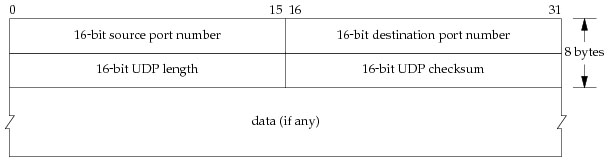
\includegraphics[scale=.7]{udp_header.jpg}
	\caption{Structura unui pachet UDP}
	\label{antetudp}
\end{figure}
%2.1.5 UDP

%2.1.6 ICMP
\subsection{ICMP}
Protocolul ICMP(Internet Control Message Protocol) este un mecanism de nivel jos folosit pentru a influen'ta comportamentul conexiunilor TCP 'si UDP. Poate fi folosit pentru a informa gazde despre o rut'a mai bun'a c'atre o anumi'ta destina'tie, a raporta o problem'a cu o anumit'a rut'a, sau a 'incheia o conexiune din cauza problemelor de re'tea. Pe l'jng'a acest lucru este folosit de cea mai important'a unealt'a de monitorizare pentru administratorii de sistem 'si de re'tele: programul ``ping''.

Multe mesaje ICMP primite de o gazd'a corespund unei anumite conexiuni sau sunt declan'sate de un pachet trimis de acea gazd'a. 'In astfel de cazuri antetul IP 'si primii 64 de bi'ti ai antetului protocolului de transport sunt incluse 'in mesajul ICMP. Astfel, un mesaj de redirec'tionare(\emph{Redirect}) sau un mesaj de 'in'stiin'tare c'a pachetul nu a putut ajunge la destina'tie(\emph{Destination Unreachable}) ar trebui s'a corespund'a unei conexiuni. Din p'acate, versiuni mai vechi de ICMP nu folosesc aceast'a informa'tie. C'jnd un astfel de mesaj este primit, toate conexiunile dintre o pereche de gazde sunt afectate 'in loc sa fie afectat'a doar conexiunea cu pricina. Acest lucru r'am'jne valabil chiar dac'a mesajul a fost declan'sat de un firewall care filtra un anumit port. Este, deci, recomandat ca firewall-urile s'a nu genereze mesaje ICMP care ar putea duce la 'incheierea for'tat'a a conexiunilor 'intre acelea'si perechi de gazde, dar pe un port legitim. Trebuie consemnat 'si faptul c'a unii cracker-i obi'snuiesc s'a abuzeze de ICMP pentru a 'incheia for'tat conexiuni; programe care exploateaz'a aceast'a vulnerabilitate exist'a.

\begin{figure}[ht]
	\centering
	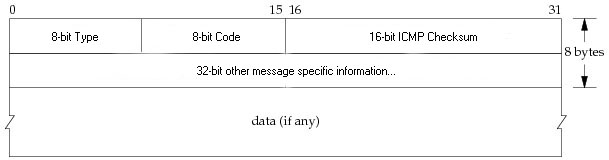
\includegraphics[scale=.7]{icmp_header.jpg}
	\caption{Structura unui pachet ICMP}
	\label{anteticmp}
\end{figure}

'Si mesajele de tip Redirect pot fi folosite 'in scopuri nefaste. Oricine care poate modifica ruta spre o anume destina'tie pe care gazda o cunoa'ste, poate probabil s'a 'ii penetreze sistemul. Doar gazdele ar tebui s'a 'tin'a cont de mesajul Redirect, nu 'si router-ele, 'si numai 'in cazul 'in care mesajul vine de la un router din re'teaua local'a. 'In orice caz, nu toate router-ele(sau, 'in unele cazuri, administratorii) sunt at'jt de atente 'in aceast'a situa'tie; este uneori posibil s'a se abuzeze de ICMP pentru a crea noi c'ai c'atre o destina'tie, ceea ce poate conduce la urm'ari nea'steptate 'si nepl'acute.
%2.1.6 ICMP
%CapII 1 Protocoalele de baza

%CapII 2 Adrese si nume
\section{Adrese 'si nume}

%2.2.1 Router-e si protocoale de rutare
\subsection{Router-e si protocoale de rutare}
Protocoalele de rutare sunt mecanisme pentru stabilirea dinamic'a a c'ailor prin Internet. Sunt in\-dis\-pen\-sa\-bi\-le opera'tiilor f'acute de TCP/IP. Informa'tia de rutare stabile'ste dou'a c'ai: de la gazda care doreste stabilirea conexiunii la destina'tie si invers. A doua rut'a este de obicei ruta inves'a; c'jnd nu se 'intampl'a a'sa, se nume'ste o cale asimetric'a 'si, 'in general, nu este un lucru bun. Dintr-o perspectiv'a a securit'a'tii, calea de 'intoarcere este, deseori, mai important'a. C'jnd o gazd'a 'tint'a este atacat'a, ruta invers'a este folosit'a pentru a transporta pachetele cu informa'tie la atacator. Dac'a un ``inamic'' poate, 'intr-un fel sau altul, s'a submineze mecanismele de rutare, atunci 'tinta poate fi f'acut'a s'a cread'a c'a sistemul ``inamic'' este, de fapt, un sistem de incredere. Dac'a asta se 'intampl'a, protocoalele de autentificare care se bazeaz'a pe verificarea adresei surs'a nu 'i'si vor 'indeplini sarcina cu succes. 

Exist'a c'jteva metode de a ataca un dispozitiv de rutare standard. Cea mai u'soar'a este de a folosi op'tiunea ``loose source route'' men'tionat'a mai sus. Astfel, persoana care ini'tiaz'a o conexiune TCP poate s'a specifice o cale explicit'a p'jn'a la destina'tie, suprascriind procesul de selec'tie a rutei care are loc 'in mod normal. A'sa cum este men'tionat 'in RFC 1122(RFC vine de la \emph{Request For Comments}; aceste documente stau la baza arhitecturii Internetului), gazda destina'tie trebuie s'a foloseasc'a calea invers'a ca rut'a de 'intoarcere, chiar dac'a are sens sau nu, ceea ce 'inseamn'a c'a un atacator poate s'a se dea drept orice gazd'a 'in care 'tinta are 'incredere.

Cel mai u'sor mod de ap'arare 'impotriva unui astfel de atac este respingerea pachetelor care con'tin op'tiunea ``loose source route''. Multe router-e asigur'a aceast'a facilitate. Op'tiunea ``loose source route'' este rareori folosit'a din motive legitime, de'si astfel de motive exist'a. De exemplu, poate fi folosit'a pentru depanarea re'telei.

O alta cale pe care atacatorii o pot aborda este s'a ``se joace'' cu protocoalele de rutare 'ins'a'si. De exemplu, este destul de usor sa se injecteze pachete care con'tin informa'tie fals'a RIP(\emph{Routing Information Protocol} este un protocol de rutare, o modalitate prin care router-ele pot comunica 'intre ele schimb'jnd informa'tie de rutare; un alt exemplu ar fi OSPF -- \emph{Open Shortest Path First}) 'intr-o re'tea. Gazdele 'si alte router-e, 'in general, vor crede aceast'a informa'tie. Dac'a sistemul atacator este mai aproape de gazda 'tint'a dec'jt adevarata gazd'a surs'a, devierea traficului se realizeaz'a u'sor.

Unele protocoale, cum ar fi RIP v2 'si OSPF, asigur'a autentificarea. Au o utilitate limitat'a din trei motive. 'In primul r'jnd, mecanismele de autentificare folosite func'tioneaz'a pe baz'a de parole; orice individ care are abilitatea s'a ``se joace'' cu protocoalele de rutare este, mai mult ca sigur, capabil s'a colecteze parolele care circul'a pe cablul re'telei. 'In al doilea r'jnd, dac'a una dintre p'ar'tile care vorbesc 'in dialogul de rutare a fost corupt'a, atunci mesajele sale sunt considerate 'in continuare legitime. 'In ultimul r'jnd, 'in majoritatea protocoalelor de rutare fiecare router comunic'a numai cu vecinii s'ai; ace'stia vor repeta ceea ce au aflat, 'in majoritatea cazurilor, f'ar'a sa critice. Ca urmare informa'tia fals'a se poate 'impr'a'stia.

Nu toate protocoalele de rutare au aceste defecte. Acelea care implic'a dialoguri 'intre perechi de gazde sunt mai greu de p'ac'alit, de'si atacuri de tipul ``sequence number attacks'', similare cu cele amintite mai devreme, pot avea succes. O defensiv'a mai puternic'a este de tip topologic. Router-ele pot, 'si ar trebui, s'a fie configurate astfel 'inc'jt s'a 'stie cu ce router-e pot comunica pe un anumit cablu(o anumit'a interfa't'a la re'tea). 'In general, acest lucru poate fi dificil, dar router-ele de tip firewall sunt pozi'tionate astfel 'inc'jt s'a implementeze aceast'a schem'a f'ar'a prea mari b'at'ai de cap.
%2.2.1 Router-e si protocoale de rutare

%2.2.2 DNS
\subsection{DNS}
DNS(Domain Name System) este un sistem distribuit de p'astrare 'si interogare a unor date arbitrare 'intr-o structur'a ierarhic'a. Cea mai utilizat'a aplica'tie a DNS este gestionarea domeniilor 'in Internet prin memorarea coresponden'telor dintre numele gazdelor 'si adresele lor IP. 'In mod normal, gazdele care vor s'a stabileasc'a o conexiune trimit o interogare UDP care con'tine numele calculatorului cu care vor s'a comunice, la servere DNS. Serverele r'aspund fie cu adresa IP dorit'a fie cu informa'tie despre servere DNS mai ``de'stepte''. Interog'arile pot fi f'acute 'si via TCP, dar opera'tiile TCP sunt, de obicei, rezervate pentru transferuri zonale(``zone transfers'' - un tip de tranzactie DNS care permite administratorilor s'a copieze bazele de date ce con'tin informa'tia DNS la mai multe servere DNS; pot fi folosite 'si de un cracker pentru a ob'tine o list'a de 'tinte rapid). 

Spa'tiile de nume au o structur'a arborescent'a. Pentru u'surin'ta opera'tiilor, subarborii pot fi aloca'ti altor servere. Doi arbori distinc'ti sunt folosi'ti. Primul asociaz'a nume cum ar fi \emph{google.ro} cu adrese precum \emph{216.239.59.104}. Alte informa'tii op'tionale(\emph{HINFO, MX}) pot fi, de asemenea, incluse. Cel de-al doilea arbore este pentru \emph{cereri inverse} 'si con'tine 'inregistr'ari de tip \emph{PTR}.

\begin{table}[ht]
	\centering
	\begin{tabular}{r|p{.6\linewidth}}
		Tip & Rol\\
		\hline
		\emph{A} & Adresa unei anumite gazde.\\
		\emph{NS} & ``Name Server''. Asociaz'a un subarbore cu un alt server.\\
		\emph{SOA} & ``Start of authority''. Desemneaz'a 'inceputul unui subarbore; con'tine cache, parametri de configurare 'si adresa persoanei responsabile pe acea zon'a\\
		\emph{MX} & ``Mail exchange''. Nume'ste gazda care proceseaz'a email-ul sosit pentru o anumit'a destina'tie.\\
		\emph{HINFO} & ``Host type and operating system information''\\
		\emph{CNAME} & Un alias pentru adev'aratul nume al unei gazde.\\
		\emph{PTR} & Folosit la maparea adreselor IP la nume ``user-friendly''.\\
	\end{tabular}
	\caption{Tipuri de inregistrari DNS}
	\label{tab:TipuriDeInregistrariDNS}
\end{table}

Nu exist'a nici o rela'tie 'intre cei doi arbori, ceea ce poate avea urm'ari nepl'acute. Un cracker care controleaz'a o por'tiune din arborele cu map'ari inverse poate modifica informa'tia din 'inregistr'ari astfel 'inc'jt s'a asocieze un nume, 'in care o anumit'a gazd'a are 'incredere, cu adresa sa IP. Apoi poate 'incerca, spre exemplu, s'a se logeze cu \emph{rlogin}(un utilitar de pe sistemele Unix care permite utilizatorilor s'a se logheze la alt'a gazd'a dintr-o re'tea, comunic'jnd via TCP pe portul 513) la gazda respectiva, care, baz'jndu-se pe falsa 'inregistrare, va accepta conexiunea.

Majoritatea sistemelor noi sunt imune la un astfel de atac. Dup'a ce primesc numele via DNS, 'il folosesc ca s'a ob'tin'a lista de adrese IP asociate cu acel nume tot via DNS. Dac'a adresa ini'tial'a nu se afl'a 'in aceast'a list'a, cerin'ta de conexiune este refuzat'a 'si o violare de securitate este logat'a.

Exist'a o variant'a mai periculoas'a a acestui tip de atac. 'In aceast'a versiune, atacatorul contamineaz'a cache-ul cu r'aspunsuri DNS al 'tintei 'inainte de a 'incerca o conexiune. Apoi intrusul ob'tine acces. O varia'tie a acestui atac include ``inundarea'' severului DNS cu r'aspunsuri false, derut'jndu-l.

De'si noile implement'ari ale protocoalelor DNS sunt imune la a'sa ceva, este imprudent s'a se cread'a ca nu mai exist'a ``g'auri'' de exploatat. Se recomand'a ca sistemele expuse la pericole s'a nu apeleze la servicii de autentificare bazate pe nume, cum ar fi rlogin. Autentificarea pe baz'a de adres'a, de'si slab'a, este mult mai sigur'a.

Exist'a un pericol 'in multe implement'ari DNS atunci c'jnd numele c'autat 'si numele utilizatorului au componente comune. De exemplu, dac'a o gazd'a cu numele \emph{foo.dept.big.edu} vrea s'a se conecteze la o destina'tie \emph{bar.com}, rezolverul DNS va 'incerca \emph{bar.com.dept.big.edu}, \emph{bar.com.big.edu} 'si \emph{bar.com.edu} 'inaite s'a 'incerce \emph{bar.com}. Aici apare riscul. Dac'a cineva ar crea un domeniu \emph{com.edu}, ar putea s'a intercepteze traficul destinat \emph{.com}.

Pe l'jng'a problemele ce 'tin de autentificare, DNS este problematic 'si la alte capitole. Con'tine mult'a informa'tie despre domenii: nume 'si adrese de gazde, structura de organizare, etc. P'astrarea acestor informa'tii astfel 'inc'jt s'a nu ajung'a 'in m'jinile ``curio'silor'' este o treab'a dificil'a. Restric'tionarea transferurilor doar la servere secundare autorizate e un bun inceput, dar atacatori inteligen'ti pot c'auta 'in mod exhaustiv spa'tiul de adrese al re'telei via cereri inverse DNS, intr'jnd 'in posesia unor liste de nume. De aici pot face alte investiga'tii ce 'ii vor conduce la aflarea altor informa'tii pre'tioase.
%2.2.2 DNS

%2.2.3 BOOTP si DHCP
\subsection{BOOTP si DHCP}

Protocolul DHCP(\emph{Dynamic Host Configuration Protocol}) este folosit pentru a asigna adrese IP 'si a furniza diferite informa'tii gazdelor abia conectate la re'tea(\emph{booting computers}). Clientul emite un pachet UDP broadcast 'si un server DHCP r'aspunde cererii. Exist'a posibilitatea ca cererile s'a fie pasate altor re'tele. Serverul poate asigna o adres'a IP fixat'a, de obicei baz'jndu-se pe adresa Ethernet a gazdei, sau poate asigna o adres'a dintr-o colec'tie de adrese disponibile. DHCP este o extensie a protocolului mai vechi 'si mai simplu, BOOTP(\emph{BOOTstrap Protocol}). 'In timp ce BOOTP livreaz'a un singur mesaj la momentul boot-'arii, DHCP asigur'a 'si notificarea eventualelor schimb'ari sau updat'ari ale adreselor IP dup'a momentul boot-'arii. Serverele DHCP pot comunica cu un server DNS pentru a asigura maparea curent'a IP/nume. 

Protocolul poate oferi destul de mult'a informa'tie: adresa serverului DNS, adresa router-ului implicit(default gateway), numele domeniului implicit, 'si, evident, adresa IP a clientului. Majoritatea implement'arilor de pe client vor folosi aceast'a informa'tie. Poate, de asemenea, s'a furnizeze adrese pentru alte tipuri de servere, cum ar fi servere NTP(Network Time Protocol), dar acestea vor fi ignorate de majoritatea implement'arilor.

Pentru re'tele de orice dimensiune este aproape imposibil s'a nu se foloseasca DHCP. Centralizeaz'a administrarea adreselor IP 'si simplific'a munca administrativ'a. Furnizeaz'a u'sor adrese IP pentru laptop-uri conectate la o re'tea wireless. Re'telele wireless trebuie s'a foloseasc'a acest protocol. 

Fi'sierele raport ale DHCP sunt foarte folositoare la investigarea atacurilor, mai ales c'jnd adresele IP sunt asignate dinamic. Este destul de important s'a se 'stie ce gazd'a a fost asociat'a cu o anumit'a adres'a IP la un moment de timp.

Protocolul este folosit 'in re'tele locale, ceea ce limiteaz'a grijile de securitate mai mult sau mai pu'tin. Gazdele care se conecteaz'a la re'tea transmit cereri 'in re'teaua local'a. Acestea pot fi pasate 'in alt'a re'tea dar serverul DHCP trebuie s'a aib'a acces la re'teaua local'a pentru c'a gazda nu 'stie 'inc'a adresa sa IP, a'sa c'a r'aspunsul trebuie dat la nivelul doi din modelul OSI, de obicei folosind adresa MAC. Deoarece acest lucru necesit'a acces la nivelul doi al unei re'tele locale, un atacator din alt'a re'tea, care nu are un astfel de acces, nu poate pune probleme.

Deoarece cererile DHCP sunt, 'in general, neautentificate, exist'a posibilitatea atacurilor de tipul \emph{man-in-the-middle} sau \emph{denial-of-service}, dar dac'a un atacator are deja acces la re'teaua local'a are op'tiunea de a folosi atacuri de tip ARP-spoofing. Ceea ce 'inseamn'a c'a folosirea BOOTP/DHCP nu adaug'a prea multe riscuri. 

Servere DHCP false pot oferi r'aspunsul mai repede dec'jt serverul oficial, astfel cre'jnd posibilit'a'ti pentru diferite atacuri, sau pot inunda serverul oficial cu cereri de la diferite adrese Ethernet simulate, consum'jnd astfel adresele disponibile.

Unele implement'ari DHCP pentru client proceseaz'a 'in mod periculos \emph{lease-ul}(perioada de timp 'in care alocarea adresei este valid'a). De exemplu, \emph{dhclient}, care ruleaz'a pe sistemele Unix, las'a un socket UDP deschis, 'si un program cu privilegii care ruleaz'a pe acea durat'a. Aceasta este o ``u's'a'' nenecesar'a pentru un eventual atac.
%2.2.3 BOOTP si DHCP
%CapII 2 Adrese si nume

%CapII 3 Transmiterea mesajelor
\section{Transmiterea mesajelor}

%2.3.1 SMTP
\subsection{SMTP}
Unul din marile avantaje pe care le aduce o conexiune la Internet unei companii este seviciul de po'st'a electronic'a. Principalul protocol folosit pentru a trimite mailuri de la un server la altul este SMPT(Simple Mail Transfer Protocol). SMTP transport'a texte compuse din caractere ASCII pe 7 bi'ti folosind un protocol relativ simplu. Iat'a un exemplu 'in Figura \ref{smtpmsg} (s'age'tile indic'a direc'tia datelor).

\begin{figure}[ht]
			\footnotesize		
			\centering
			
			\begin{description}
				\item[$<---$] 220 inet.att.com SMTP
				\item[$--->$] HELO A.SOME.EDU
				\item[$<---$] 250 inet.att.com
				\item[$--->$] MAIL FROM:$<$Ferd.Berfle@A.SOME.EDU$>$
				\item[$<---$] 250 OK
				\item[$--->$] RCPT TO:$<$mark.farkle@research.att.com$>$
				\item[$<---$] 250 OK
				\item[$--->$] DATA
				\item[$<---$] 354 Start mail input; end with $<$CRLF$>$.$<$CRLF$>$
				\item[$--->$] From Ferd.Berfle@A.SOME.EDU Thu Jan 27 21:00:05 EST 1994
				\item[$--->$] From: Ferd.Berfle@A.SOME.EDU
				\item[$--->$] To: mark.farkle@research.att.com
				\item[$--->$] Date: Thu, 27 Jan 94 21:00:05 EST
				\item[$--->$] 
				\item[$--->$] Meet you for lunch after the meeting with Sparkle.
				\item[$--->$] 
				\item[$--->$] Ferd
				\item[$--->$] .
				\item[$--->$] 
				\item[$<---$] 250 OK
				\item .... A.SOME.EDU!Ferd.Berfle sent 273 bytes to research.att.com!mark.farkle
				\item[$--->$] QUIT
				\item[$<---$] 221 inet.att.com Terminating
			\end{description}
			\caption{Exemplu de mesaj SMTP}
			\label{smtpmsg}
\end{figure}

'In cazul de fa'ta serverul A.SOME.EDU transfer'a un email la gazda INET.ATT.COM. 'In comanda ``MAIL FROM'' este specificat'a adresa email a transmi'tatorului. 'In acest moment nu exist'a nici un mod pentru gazd'a s'a verifice aceast'a adres'a. Nu se 'stie 'in mod cert cine a trimis emailul 'in contextul SMTP. Trebuie folosit un mecanism de nivel mai 'inalt dac'a este nevoie de 'incredere 'si protejarea intimit'a'tii. 'In practic'a organiza'tiile folosesc de obicei un \emph{emai gateway} chiar dac'a re'telele componente sunt conectate la Internet. Gateway-ul se poate asigura c'a antetele de email care sunt trimise respect'a standardele.

Din punct de vedere al securit'a'tii, protocolul SMPT, de unul singur, este destul de inofensiv. 'In unele cazuri poate fi sursa unor atacuri de tip DoS(Denial-of-service), discutate mai t'jrziu.

Una dintre cele mai comune implement'ari ale SMTP este reprezentat'a de programul \emph{sendmail}, inclus 'in majoritatea distribu'tiilor de Unix. Sendmail a ap'arut 'in zilele de 'inceput ale Internetului, pe vremea c'jnd securitatea nu era o considera'tie primar'a 'in contextul dezvolt'arii unei aplica'tii pentru re'tele. A'sadar, primele versiuni ale acestui program aveau nenum'arate g'auri de securitate, at'jt inten'tionate c'jt 'si neinten'tionate(con'tine zeci de mii de linii de cod 'in limbajul C 'si ruleaza ca root - programele privilegiate ar trebui s'a fie c'jt mai mici 'si mai modulare posibil). Una din aceste g'auri a fost exploatat'a de a'sa-numitul \emph{Internet Worm}, cunoscut 'si sub numele de \emph{Morris worm}(unul dintre primii viermi rasp'jndi'ti prin Internet). Un serviciu SMTP nu are nevoie s'a aib'a privilegii de root.

Nu numai c'a SMPT nu are un mecanism real de securitate, dar modelul SMTP, fiind construit 'in zilele de 'inceput ale Internetului, este 'in intregime construit 'in jurul ideii de ``cooperare'' 'si ``'incredere'' 'intre severe. Deoarece majoritatea serverelor SMTP trebuiau s'a medieze un anumit num'ar de trasferuri, fiecare server era obligat s'a accepte mail de la orice surs'a 'si s'a il livreze la orice destina'tie. Principala presupunere 'in acest model este c'a toate serverele SMTP se vor comporta ``bine'' 'si nu vor abuza de sistem inund'jnd alte servere cu multe mailuri ce trebuiesc livrate sau trimi't'jnd mesaje false pentru a cauza probleme. Acest lucru s-a schimbat odata cu explozia Internetului 'in anii 1990. Farseurii, cracker-ii, chiar 'si unii agen'ti de marcheting au decoperit c'a e-mailul ar putea fi folosit ``gratis'' pentru a trimite mesaje pur 'si simplu prin trasnmiterea lor unor servere SMTP pentru livrare. Rezultatul a constat 'in supra'inc'arcarea serverelor din cauza cantit'a'tilor mari de mesaje nedorite, cunoscute 'si sub numele de \emph{spam}.

'In alt'a ordine de ideei, este destul u'sor pentru un sistem s'a ``se dea drept'' un server SMTP. Se poate folosi protocolul \emph{Telnet} pentru o conexiune direct'a la un server SMTP pe portul 25. Comenzile SMTP sunt timise ca text(a'sa cum am ar'atat mai sus), la fel 'si r'aspunsurile SMTP, ceea ce 'inseamn'a c'a se poate ``conversa'' cu un server SMTP chiar prin introducerea comenzilor manual. Acest lucru este folositor pentru depanare, dar poate fi folosit 'si 'in mod abuziv. Deoarece a'sa-numi'tii ``spammeri'' nu vor s'a fie identifica'ti, folosesc tehnici bazate pe \emph{spoofing} pentru a 'ingreuna depistarea.

Deoarece e-mailul este destul de des abuzat 'in ziua de azi, majoritatea serverelor SMTP moderne 'incorporeaz'a un mecanism de securitate pentru a evita problemele.
%2.3.1 SMTP

%2.3.2 MIME
\subsection{MIME}
MIME(Multipurpose Internet Mail Extensions) este un standard care extinde formatul unul e-mail adaug'jnd posibilitatea de a trimite: texte scrise cu alte seturi de caractere 'in afar'a de ASCII, ata'samente non-text, mesaje multi-part, etc. Practic, toate e-mailurile scrise de un utilizator 'si trimise pe Internet, c'jt 'si o mare parte din e-mailurile trimise automat, sunt transmise via SMTP 'in format MIME.

Con'tinutul unui e-amil poate pune la r'jndul lui probleme. 'In afar'a de posibile bug-uri 'in programul de mail al gazdei destina'tie, executarea automat'a a mesajelor MIME este un poten'tial pericol. Informa'tia codat'a 'in aceste mesaje poate indica ac'tiuni ce trebuiesc executate. O bucat'a dintr-un posibil e-mail MIME este reprezentat'a mai jos.

\begin{figure}[ht]
	\footnotesize
	
	Content-Type:$   $Message/External-body;\\
	name=''rfc2549.txt'';\\
	site=''ftp.isi.edu'';\\
	access-type=''anon-ftp'';\\
	directory=''in-notes''\\
	Content-Type: text-plain
\end{figure}

Un program de mail care cunoa'ste MIME ar desc'arca fi'sierul specificat automat. S'a presupunem c'a un atacator ar trimite urm'atorul mesaj:

\begin{figure}[ht]
	\footnotesize
	
	Content-Type:$   $Message/External-body;\\
	name=''.rhosts'';\\
	site=''ftp.evilhacker.org'';\\
	access-type=''anon-ftp'';\\
	directory=''.''\\
	Content-Type: text-plain
\end{figure}

Va suprascrie agentul MIME actualul fi'sier \emph{.rhosts}(con'tine o list'a de gazde 'si utilizatori 'in care gazda local'a are ``'incredere'' c'jnd o conexiune e f'acut'a folosind serviciul \emph{rshd}) din directorul curent? Va observa utilizatorul c'a ceva e suspicios dac'a textul mesajului pare legitim?

O implementare MIME permite ca un mesaj s'a fie fragmentat 'in p'ar'ti multiple. O astfel de fragmentare poate fi folosit'a pentru a trece de eventualii antiviru'si de pe gateway-uri. Desigur, acest lucru nu ar putea fi dus la bun sfar'sit dac'a programul de mail al destina'tiei nu ar putea reasambla fragmentele; Microsoft Outlook Express face acest lucru 'si a fost cauza multor infec'tii 'in mas'a cu \emph{viermi}(worms). Evitarea acestui scenariu se poate face fie prin reasamblarea la nivelul gateway-ului fie prin respingerea mesajelor fragmentate.

Alte pericole puse de MIME constau 'in abilitatea de a trimite prin mail programe executabile sau alte tipuri de fi'siere care pot la r'jndul lor cauza ac'tiuni periculoase. 'Intr-adevar, posibilitatea trimiterii de con'tinut activ prin e-mail este un factor primar 'in r'asp'jndirea viermilor 'si viru'silor.
%2.3.2 MIME

%2.3.3 POPv3
\subsection{POPv3}
POP3(\emph{Post Office Protocol version 3}) este folosit de clien'ti pentru a ob'tine mesajele e-mail de la server. E-mailurile utilizatorilor serviciului de mail sunt stocate pe un server(posibil al ISP-ului). C'jnd un client ruleaz'a programul de mail, acesta download-eaz'a mesajele de pe server. 'In mod normal mesajele desc'arcate sunt 'sterse de pe server. C'jt timp ruleaz'a, programul de mail poate trimite cereri repetate la intervale regulate de timp pentru a ob'tine poten'tiale noi mesaje. Clientul trimite mail folosind SMTP.

Protocolul este destul de simplu 'si exist'a de ceva timp. Serverul 'il poate implementa u'sor, chiar 'si cu un script de \emph{Pearl}(limbaj de scriptare).

POP3 este destul de nesigur. 'In versiuni mai vechi, parola utilizatorului era transmis'a f'ar'a suspiciuni pentru a ob'tine acces la ``cutia po'stal'a''(mail box). Implemet'arile mai noi folosesc comanda APOP pentru autentific'ari pe baz'a de parol'a(schimburi \emph{Challenge/response}). Acest tip de autentificare permite un atac ``cu dic'tionar'' asupra parolei. Unele site-uri suport'a POP3 peste SSL/TLS(\emph{Secure Sockets Layer/Transport Layer Security} - protocoale criptografice care asigur'a comunica'tii securizate pe Internet). Din p'acate nu se poate spune acela'si lucru 'si despre majoritatea programelor de mail pentru client.

Daca serverul ruleaz'a Unix, 'in mod normal, programul POP3 pentru server va rula ca \emph{root} p'jn'a ce autentificarea este complet'a, apoi 'i'si va schimba contul 'in contul utilizatorului de pe server. Ceea ce 'inseamn'a c'a utilizatorul trebuie s'a aibe un cont pe server, lucru neindicat pentru c'a implic'a mai mult'a munc'a administrativ'a 'si faptul c'a un utilizator se poate loga la server el 'insu'si. Acest lucru nu este niciodat'a o idee bun'a: ``utilizatorii sunt riscuri mari de securitate''. 

Beneficiile POP3 includ simplitatea protocolului 'si u'surin'ta implement'arii pentru server.
%2.3.3 POPv3

%2.3.4 IMAPv4
\subsection{IMAPv4}
IMAP(\emph{Internet Message Access Protocol}) versiunea 4 ofer'a acces de la distan't'a la ``cutiile po'stale'' de pe un server de e-mail. Permite clientului 'si serverului s'a sincronizeze starea 'si asigur'a suport pentru fi'siere multiple. Ca 'si la POP3, mesajele sunt trimise folosind protocolul SMTP.

Protocolul IMAP suport'a o suit'a de metode de autentificare, 'in care se g'asesc 'si c'jteva destul de sigure. Autentificarea de tip ``challange/response'' e un pas 'in direc'tia bun'a. Cu toate acestea, un secret partajat este implicat, care trebuie stocat pe server.

Cel mai mare dezavantaj al lui IMAP este complexitatea protocolului, ceea ce implic'a o implementare complexa a programului de server. Dac'a partea de server este implementat'a cum se cuvine, cu un modul de autentificare simplu ca ``front-end'' la programul principal ce trebuie s'a ruleze neprivilegiat, atunci pericolele sunt la fel de reduse ca 'si 'in cazul unei log'ari de utilizator. 
%2.3.4 IMAPv4

%2.3.5 IM
\subsection{IM}
Exist'a multe programe comerciale de \emph{Instant Messaging} care folosesc protocoale private. AOL Instant Messenger folose'ste o conexiune TCP la un \emph{server farm}(o colec'tie de servere) pentru a lega clien'tii 'intre ei. ICQ procedeaz'a la fel. Se poate presupune c'a serviciile de mesagerie instant'a opereaz'a 'in modul \emph{peer-to-peer} de la un momentdat(de exemplu dup'a ce doi clien'ti 'si-au aflat adresele unul celuilalt), dar este pu'tin probabil ca acest mod de comunicare s'a func'tioneze dac'a ambii utilizatori se afl'a 'in spatele unui firewall. Programul client are de obicei 'si alte feature-uri cum ar fi abilitatea de a face schimb de fi'siere, suportul pentru camere web 'si microfon, etc. Bug-uri de securitate au ap'arut ca urmare a complexit'a'tii sporite 'in unele implement'ari.
%2.3.5 IM
%CapII 3 Transmiterea mesajelor


%capII 4 Protocoale bazate pe RPC
\section{Protocoale bazate pe RPC}

%2.4.1 RPC si portmapper / rpcbind
\subsection{RPC 'si \emph{Portmapper}}
%http://en.wikipedia.org/wiki/Rpc
RPC(\emph{Remote Procedure Call}) este o tehnologie care permite unui program ce se execut'a pe un calculator s'a apeleze o subrutin'a dintr-un alt spa'tiu de adresare(adic'a nu memoria local'a), 'in general, de pe alt calculator aflat 'in accea'si re'tea, f'ar'a ca programatorul s'a codeze explicit aceast'a interac'tiune. 'In paradigma program'arii orientate pe obiecte se folose'ste termenul RMI(\emph{remote method invocation}). Prima implementare popular'a a RPC pe Unix a apar'tinut \emph{Sun Microsystems} 'si se nume'ste 'in prezent \emph{ONC RPC}. Alte exemple sunt \emph{NCS}, \emph{DCE/RPC} 'si \emph{MSRPC}(Microsoft RPC).

Protocolul RPC st'a sub multe dintre noile servicii. Din nefericire, multe dintre aceste servicii prezint'a poten'tiale probleme de securitate.

Conceptul de baz'a este destul de simplu. O persoan'a care dezvolt'a un serviciu de re'tea folose'ste un limbaj special pentru a specifica numele func'tiilor ce se vor executa pe alt calculator 'si parametrii acestora. Un precompilator transform'a aceast'a specifica'tie 'in module at'jt pentru client c'jt 'si pentru server. 'In acest fel clientul poate apela o subrutin'a de pe server 'in mod transparent; majoritatea dificult'a'tilor de programare pentru re'tea sunt mascate de nivelul RPC.

RPC poate fi a'sezat at'jt peste TCP c'jt 'si peste UDP; dar un sistem care folose'ste RPC a'sezat peste UDP trebuie s'a aib'a 'in vedere mesaje pierdute, duplicate, amestecate, etc.

Mesajele RPC au antetul(Figura \ref{antetrcp}) lor propriu care include, printre altele, num'arul programului, num'arul procedurii, 'si versiunea.

\begin{figure}[ht]
	%http://www.rhyshaden.com/rpc.htm
	\centering
	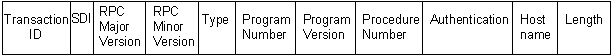
\includegraphics[scale=.7]{rpc_header.jpg}
	\caption{Antetul unui mesaj RPC a'sezat peste TCP}
	\label{antetrcp}
\end{figure}

Exist'a 'si o sec'tiune a antetului destinat'a autentific'arii, dar este posibil'a 'si folosirea anonim'a a serviciilor. Pentru servicii ``mai serioase'', a'sa-numitul c'jmp de autentificare Unix este folosit. Acesta include id-ul utilizatorului 'si id-ul grupului apelatorului, 'si numele sistemului de unde se face apelul procedurii. Numele sistemului nu ar trebui niciodat'a luat 'in calcul('si servicii importante cum ar fi NFS - \emph{Network File System} - 'il ignor'a 'in favoarea adresei IP), 'si nici celelalte dou'a c'jmpuri nu garanteaz'a prea mult dec'jt dac'a mesajul este de pe un port privilegiat; chiar 'si atunci nu 'inseamn'a mare lucru dac'a RPC-ul este bazat pe UDP('in acest caz falsificarea unei adrese este trivial'a). 

RPC suport'a autentificare pe baz'a de criptare folosind DES(Data Encryption Standard), in acest caz fiind numit uneori \emph{Secure RPC}. Toate apelurile sunt autentificate folosind o cheie de sesiune. Cheile de sesiune sunt distribuite folosind protocolul criptografic \emph{Diffie-Hellman exponential key exchange}(protocol ce permite stabilirea unei chei 'intre dou'a p'ar'ti, care ini'tial nu aveau cuno'stin'te una despre cealalt'a, printr-un canal nesigur).

Din nefericire protocolul RPC cu autentificare bazata pe DES nu este bine integrat 'in majoritatea sistemelor. NFS este singurul protocol standard care 'il folose'ste. Mai este folosit 'in unele versiuni de Telnet 'si FTP.

DCE/RCP(Distributed Computing Environment) folose'ste autentificare DES dar cu \emph{Kerberos} ca mecanism de distribuire a cheilor. Cu oricare dintre cele doua tipuri de autentificare gazda trebuie s'a re'tin'a 'intr-un cache datele de autentificare. Mesajele viitoare ar putea con'tine un pointer c'atre locul unde au fost re'tinute datele. Trebuie 'tinut cont de acest lucru c'jnd se 'incearc'a analizarea sau filtrarea mesajelor RPC.

Restul unui mesaj RPC const'a 'in parametrii pentru procedura de invocat sau rezultatul 'intors de aceasta. Acestea sunt codate folsind protocolul XDR(External Data Representation).

Cu excep'tia NFS, serviciile bazate pe RPC nu folosesc porturi prestabilite. Accept'a orice port care le este oferit de sistemul de operare 'si 'il 'inregistreaz'a cu \emph{portmapper}. Portmapper -- care el 'insu'si folose'ste protocolul RPC -- se comport'a ca un intermediar 'intre clien'tii 'si serverele RPC. Pentru a contacta un server, clientul 'intreaba mai 'int'ji portmapper-ul de pe server care este portul 'si protocolul(TCP sau UDP) serviciului pe care vrea s'a 'il foloseasc'a. Aceast'a informa'tie este folosit'a apoi pentru cererea de conexiunea RPC propriu-zis'a.

Portmapper-ul are 'si alte abilit'a'ti mai periculoase din punct de vedere al securit'a'tii. De exemplu, exist'a un tip de cerere pentru a 'sterge un serviciu din list'a care reprezint'a o poten'tial'a 'tint'a a atacurilor de denial-of-service deoarece 'ii lipse'ste autentificarea. Portmapper-ul este, de asemenea, ``fericit'' s'a spun'a oricui din re'tea ce servicii ofer'a gazda respectiv'a, ceea ce este foarte folositor atunci c'jnd se 'incearc'a un atac.

Cea mai serioas'a problem'a a portmapper-ului este reprezentat'a de abilitatea pe care o include de a trimite cereri indirecte. Pentru a face economie de timp, clientul poate s'a cear'a portmapper-ului s'a 'inainteze cererea serviciului propriu-zis, f'ar'a s'a mai trimit'a num'arul portului la client. Dar mesajul 'inaintat poart'a adresa portmapper-ului, ceea ce face imposibil pentru aplica'tii s'a recunoasc'a dac'a mesajul este o cerere local'a sau nu, 'si, ca urmare, s'a stabileasc'a nivelul de 'incredere pe care s'a il acorde cererii.

Unele versiuni de portmapper fac propria lor filtrare. 'In cazul 'in care nu se 'intampl'a acest lucru, este bine ca nici un strain sa nu 'il poat'a accesa. Acest lucru 'ins'a nu va bloca accesul la serviciile propriu-zise; este foarte u'sor pentru un atacator s'a scaneze spa'tiul de porturi direct.

\begin{figure}[ht]
		\footnotesize		
			\centering
			\begin{tabular}{llllp{.6\linewidth}}
				program & vers & proto & port\\
				100000 & 2 & tcp & 111& portmapper\\
				100000 & 2 & udp & 111& portmapper\\
				100029 & 1 & udp & 656& keyserv\\
				100026 & 1 & udp & 729& bootparam\\
				100021 & 1 & tcp & 735& nlockmgr\\
				100021 & 1 & udp & 1029& nlockmgr\\
				100021 & 3 & tcp & 739& nlockmgr\\
				100021 & 3 & udp & 1030& nlockmgr\\
				100020 & 2 & udp & 1031& llockmgr\\
				100020 & 2 & tcp & 744& llockmgr\\
				100021 & 2 & tcp & 747& nlockmgr\\
				100021 & 2 & udp & 1032& nlockmgr\\
				100024 & 1 & udp & 733& status\\
				100024 & 1 & tcp & 736& status\\
				100011 & 1 & udp & 3739& rquotad\\
				100001 & 2 & udp & 3740& rstatd\\
				100001 & 3 & udp & 3740& rstatd\\
				100001 & 4 & udp & 3740& rstatd\\
				100002 & 1 & udp & 3741& rusersd\\
				100002 & 2 & udp & 3741& rusersd\\
				100012 & 1 & udp & 3742& sprayd\\
				100008 & 1 & udp & 3743& walld\\
				100068 & 2 & udp & 3744
			\end{tabular}
	\caption{Exemplu de output portmapper}
	\label{portmapperdump}
\end{figure}

Chiar 'si f'ar'a probleme induse de portmapper, serviciile RPC au o istorie plin'a de probleme de securitate. Majoritatea au fost scrise pentru a rula pe calculatoare conectate doar la o re'tea Ethernet, f'ar'a acces la Internet, deci f'ar'a prea mari m'asuri de precau'tie. 
%2.4.1 RPC si portmapper / rpcbind

%2.4.2 NIS
\subsection{NIS}
Una din cele mai periculoase aplica'tii bazate pe RPC este NIS(\emph{Network Information Service}), cunoscut'a mai 'int'ji ca YP(\emph{Yellow Pages}. NIS este folosit pentru a distribui o varietate de baze de date importante de la un server central la clien'ti. Acestea pot fi fi'sierul cu parole, tabela cu adrese, bazele de date cu chei publice 'si private folosite la Secure RPC, etc.. 

Majoritatea riscurilor sunt evidente. Despre un intrus care ob'tine fi'sierul cu parole se poate spune c'a a ob'tinut un lucru pre'tios. Baza de date cu chei poate fi aproape la fel de pre'tioas'a. 

S'a consider'am un site care nu neglijeaz'a securitatea 'si care folose'ste a'sa-numitul \emph{shadow password file}(un mecanism utilizat pentru a cre'ste nivelul de securitate al parolelor pe sistemele de tip Unix prin interzicerea accesului la fisierul cu parole pentru utilizatorii obi'snui'ti; 'in mod normal ace'stia au drepturi de citire). Un astfel de fi'sier 'tine parolele codate(\emph{hashed}). Dar astfel de sisteme au nevoie de un mecanism prin intermediul c'aruia aplica'tiile s'a valideze parolele. Acest lucru este f'acut folosind un serviciu bazat pe RPC; acest serviciu nu raporteaz'a rate ridicate de cereri, a'sa cum ar putea fi generate de un atacator.

Clien'tii NIS trebuie s'a aib'a cuno'stin't'a 'si despre servere backup, 'in caz c'a serverul principal se stric'a. 'In unele versiuni, clien'tilor li se spune, de la distan't'a, s'a foloseasc'a un server diferit, posibil fraudulos. Acest ``server'' ar putea trimite informa'tii false din \emph{/etc/passwd}, adrese incorecte, etc.

Unele versiuni ale acestui protocol pot fi configurate s'a nu accepte activit'a'ti periculoase. Cel mai sigur este s'a nu se folosesc'a NIS pe sistemele expuse deoarece riscurile sunt mari 'si, 'in cazul nodurilor gateway, avantajele nu compenseaz'a.
%2.4.2 NIS

%2.4.3 NFS
\subsection{NFS}
Un sistem de fi'siere re'tea(\emph{network file system}) este orice sistem de fi'siere care permite partajarea fi'sierelor, imprimantelor 'si a altor resurse 'intr-o re'tea de calculatoare.

Protocolul NFS(\emph{Network File System}), creat de \emph{Sun Microsystems}, este acum suportat pe majoritatea calculatoarelor. Este o component'a vital'a pentru sta'tiile de lucru specializate, 'si este putin probabil s'a fie 'inlocuit in viitorul apropiat.

Pentru robuste'te, NFS este bazat pe RPC, UDP 'si servere \emph{stateless}(f'ar'a stare). Asta 'inseamn'a c'a pentru serverul NFS - adic'a gazda unde se g'asesc fi'sierele partajate - fiecare cerere este independent'a, nu este re'tinut un anumit context. Ca urmare, fiecare opera'tie trebuie autentificat'a individual, lucru ce poate ridica unele probleme.

Pentru a face accesul NFS robust 'in fa'ta restart'arii sistemelor 'si parti'tion'arii re'telei('imp'ar'tirea 'in subre'tele 'si aplicarea filtrelor 'intre acestea), clien'tii re'tin starea, serverele nu. Fiecare fi'sier sau director stocat pe disc este indentificat 'in mod unic de un 'sir de caractere. Orice cerere NFS const'a dintr-un astfel de 'sir, o opera'tie 'si parametrii necesari pentru acea opera'tie. Cererile care permit acces la noi fi'siere, cum ar fi \emph{open}, intorc un nou indentificator la procesul client. 

Identificatorul ini'tial, pentru directorul r'ad'acin'a este ob'tinut la momentul mont'arii sistemului de fi'siere. Nu trebuie trecute cu vederea implica'tiile acestui fapt. Orice client care re'tine identificatorul pentru fi'sierul r'ad'acin'a are acces permanent la sistemul de fi'siere. De'si programele client standard renegociaz'a accesul la fiecare montare(care are loc de obicei la reboot-are), acest lucru nu este impus. Din acest motiv, serverele NFS bazate pe GSS-API(Generic Security Services Application Program Interface - un standard IETF pentru sistemele de securitate), vor verifica drepturile de acces la fiecare opera'tie.

Identificatorii de fi'siere sunt, 'in mod normal, asigna'ti la momentul cre'arii sistemului de fi'siere, prin intermediul unui generator de numere pseudoaleatoare. (Unele versiuni mai vechi de NFS foloseau o s'am'jn't'a ``nesuficient'' de aleatoare(previzibil'a); rapoarte indic'a faptul c'a au avut loc atacuri 'incheiate cu succes.)

Unele opera'tii de sisteme de fi'siere pe Unix, cum ar fi restric'tionarea accesului la fi'siere sau 'inregistrare (\emph{file/record locks}), necesit'a p'astrarea st'arii pe server, indiferent de arhitectura NFS. Aceste opera'tiuni sunt implementate de procese auxiliare, folosind RPC. Serverele folosesc astfel de mecanisme 'si pentru a 'tine eviden'ta clien'tilor care au montat sistemul de fi'siere.

NFS se bazeaz'a 'in general pe un set de identificatori numerici de utilizatori 'si grupuri care trebuie s'a fie consistent peste mul'timea de clien'ti. Convenient pentru uz local, nu este o solutie scalabil'a. Accesul ca \emph{root} este, 'in general, restric'tionat, ceea ce aduce deseori mai mult'a frustrare dec'jt protec'tie.

'In mod normal, serviciile NFS se acceseaz'a pe portul 2049. Alegerea portului este problematic'a deoarece se afl'a 'in zona ``neprivilegiat'a'', 'si ca atare acest num'ar de port poate fi asignat unui proces normal. Filtrele de pachete care permit conversa'tii UDP trebuiesc configurate s'a blocheze accesul la portul 2049; serviciul este prea periculos. Mai mult dec'jt at'jt, unele versiuni de NFS 'i'si asigneaz'a porturi aleatoare, folosind \emph{rpcbind} pentru informa'tii de adresare.

NFS pune probleme de securitate 'si clien'tilor. Cineva cu acces privilegiat la server(sau cineva care poate asambla pachete r'aspuns), poate crea programe \emph{setuid}('in Unix, op'tiune de drepturi de acces care permite utilizatorilor s'a ruleze un fi'sier executabil cu permisiunile de'tin'atorului fi'sierului), ca mai apoi s'a le ruleze de pe calculatorul clientului. Unele implement'ari NFS au op'tiunea de a bloca astfel de importuri. 

O problem'a mai subtil'a 'in ceea ce prive'ste navigarea prin arhive via NFS este reprezentat'a de faptul c'a este destul de u'sor pentru server s'a planteze versiuni capcan'a ale diferitelor programe, cum ar fi \emph{ls}. Dac'a 'in variabila \emph{path} prima cale este directorul curent, versiunea capcan'a va fi folosit'a 'in locul comenzii ls a clientului. Dac'a directorul curent apare 'in variabila path, ar trebui s'a fie 'intotdeauna ultimul. Cea mai bun'a defensiv'a ar fi ca programul NFS client s'a 'stearg'a bitul de ``executare'' al tuturor fi'sierelor importate. Nu exist'a clien'ti standard NFS care s'a asigure aceast'a op'tiune. 

Multe site-uri folosesc acum versiunea 3. Cel mai notabil atribut este posibilitatea func'tion'arii peste TCP, ceea ce face autentific'arile mai u'soare.
%2.4.3 NFS
%capII 4 Protocoale bazate pe RPC


%capII 5 Protocoale pentru transfer de fisiere
\section{Protocoale pentru transfer de fi'siere}
%2.5.1 TFTP
\subsection{TFTP}
TFTP(\emph{Trivial File Transfer Protocol}) este un protocol simplu, a'sezat peste UDP. Nu con'tine un mecanism de autentificare. Este deseori folosit de rutere, sta'tii de lucru f'ar'a unit'a'ti de disc 'si terminale X11.

Un serviciu TFTP configurat cum se cuvine restric'tioneaz'a transferul de fi'siere pentru anumite directoare speciale. Mai de mult, majoritatea companiilor eliberau produsele software cu acces TFTP nerestric'tionat, ceea ce f'acea munca unui hacker mai u'soar'a, acest'a put'jnd, prin comenzi TFTP, s'a transfere f'ar'a prea mult efort fi'siere importante cum ar fi /etc/passwd. Din acest motiv este recomandat s'a nu se foloseasc'a TFTP dec'jt 'in cazuri inevitabile, 'si, dac'a se folose'ste, s'a fie configurat corect astfel 'inc'jt s'a livreze doar fis'ierele corespunzatoare, doar clien'tilor corespunz'atori.

Multe router-e folosesc TFTP pentru a-'si 'inc'arca fi'siere de configura'tie, ceea ce reprezint'a iara'si un pericol deoarece, deseori, acestea con'tin parole. Serviciul TFPT ar trebui setat astfel 'inc'jt doar router-ul 'in cauz'a s'a poat'a comunica cu el.
%2.5.1 TFTP

%2.5.2 FTP
\subsection{FTP}
FTP(\emph{File Transfer Protocol}) permite transmiterea de fi'siere binare 'si text, cu eventuala conversie a setului de caractere pentru cele de tip text. 'Intr-o sesiunea obi'snuit'a, clientul deschide un canal de control c'atre server care a'steapt'a conexiunea pe portul 21. Diverse comenzi 'si r'aspunsuri sunt transmise pe acest canal. R'aspunsurile serverului includ un cod de trei cifre la 'inceputul fiec'arei linii.

Un al doilea canal, de date, este deschis pentru transferul propriu-zis al fi'sierelor. Specifica'tia protocolului FTP sugereaz'a ca un singur canal s'a fie creat 'si p'astrat deschis pentru toate transferurile de date dintr-o sesiune. 'In practic'a, implementarile FTP deschid un nou canal pentru fiecare fi'sier transferat.

Se diferen'tiaz'a dou'a moduri de creare a canalului de date: de la server c'atre client(mod activ) 'si de la client c'atre server(mod pasiv). Aceast'a alegere are importante implica'tii de securitate. 'In cazul modului activ, clientul ascult'a pe un port aleator 'si informeaz'a serverul despre acest lucru pe canalul de control prin comanda \emph{PORT}. Serverul se conecteaz'a la portul primit, de obicei folosind ca port local portul 20. Conexiunea pentru transferul datelor poate fi deschis'a de la client la server ca 'in cazul canalului de control. Clientul trimite comanda \emph{PASV} serverului, serverul ascult'a pe un port oarecare 'si informeaz'a clientul despre portul 'in cauz'a 'in r'aspunsul la comanda PASV. 

Majoritatea serverelor FTP de pe Internet suport'a comanda PASV. Mul'ti clien'ti FTP au fost modifica'ti s'a o foloseasc'a(o modificare simpl'a: 'in jur de 10 linii de cod) 'si toate browser-ele importante o suport'a. Motivul acestui lucru este c'a vechea comand'a PORT prin care se inverseaz'a direc'tia canalului face stabilirea politicii de securitate mult mai dificil'a, complic'jnd construirea firewall-urilor 'si diminu'jnd siguran'ta adus'a de acestea. Este destul de u'sor 'si, de asemenea, rezonabil s'a se implementeze un firewall care permite conexiuni TCP spre exterior(outgoing) dar nu 'si dinspre exterior spre interior(incoming). Dac'a comanda PORT este suportat'a, este nevoie de un mecanism care s'a permit'a aceste cereri dinspre exterior.

Exist'a 'si pericole 'in implementarea unui astfel de mecanism. Dac'a un atacator vrea s'a se conecteze, s'a zicem, la portul telnet(23) al unei gazde din spatele unui firewall, poate folosi un program care s'a se dea drept un client FTP(de exemplu, un applet Java pe un site); s'a presupunem c'a victima execut'a acest program; 'in acest moment programul deschide o conexiune FTP 'inapoi la atacator 'si trimite o comand'a PORT specific'jnd portul 23 pe gazda 'tint'a. Firewall-ul va fi neputincios 'in acest moment l'as'jnd portul liber din cauza mecanismului implementat pentru a permite conexiuni active FTP. Solu'tia poate fi ignorarea comenzii PORT sau asigurarea c'a firewall-ul nu va l'asa deschise porturi privilegiate. De asemenea este indicat'a asigurarea c'a adresa specificat'a 'in comanda PORT este aceea'si cu cea a gazdei de unde a fost trimis'a.

Pe l'jng'a dificultatea trat'arii cererilor de conexiune dinspre exterior comanda PORT mai pune 'si alt'a problem'a: atacul \emph{FTP Bounce}. Acest tip de atac se bazeaz'a pe faptul c'a un atacator poate spune unei gazde s'a deschid'a o conexiune pe un port arbitrar spre o alt'a gazd'a arbitrar'a.

Implicit, transferurile FTP sunt f'acute 'in mod ASCII. 'Inainte de a trimite sau primi un fi'sier care con'tine caractere nonprintabile ASCII, ambele par'ti trebuie s'a intre 'in mod binar prin comanda \emph{TYPE I}.

De'si PASV este preferabil, se pare c'a PORT nu va fi abandonat. Majoritatea firewall-urilor suport'a aceast'a comand'a 'si este comportamentul implicit al noilor programe Microsoft.

FTP anonim(Anonymous FTP) este un mecanism destul de important de distribu'tie de date. Site-urile care doresc pot configura serverele FTP s'a permit'a ``str'ainilor'' s'a downloadeze fi'siere dintr-o arie restric'tionat'a f'ar'a prearanjamente, autoriza'tie sau autentificare. Prin conven'tie, utilizatorii se conecteaz'a cu numele \emph{anonymous} pentru a folosi serviciul. Unele site-uri cer ca adresa de po'sta electorinic'a a utilizatorului s'a fie folosit'a ca parol'a.

FTP prezint'a 'si o serie de dezavantaje:
\begin{itemize}
	\item Dac'a nu este configurat a'sa cum se cuvine, serviciul poate permite accesul la fi'siere importante ale unei companii.
	\item Parolele 'si con'tinutul sunt trimise ca text clar ceea ce 'inseamn'a c'a pot fi citite de o persoan'a din re'tea care folose'ste un Sniffer.
	\item Au existat diverse bug-uri 'in implement'arile serviciilor care au deschis multe g'auri de securitate.
	\item Directoarele cu drept de scriere 'in FTP anonim sunt des folosite pentru a stoca 'si distribui \emph{warez}(softwere furat sau alte date ilicite)
\end{itemize}

Pe de alt'a parte, FTP anonim a devenit un standard important pe Internet pentru publicarea de soft, articole, poze, etc. Multe site-uri trebuie s'a asigure accesul public prin FTP anonim. De'si, 'in mare parte, aceste nevoi sunt satisf'acute de Web, FTP reprezint'a inc'a cea mai bun'a metod'a pentru upload de fi'siere. Nu exist'a nici o 'indoial'a c'a FTP anonim este un serviciu valoros, ins'a trebuie administrat cu mult'a grij'a.

Prima 'si cea mai important'a regul'a este c'a \emph{ftp login} nu trebuie sa aib'a drepturi de scriere sau s'a fie proprietarul niciunui fi'sier sau director de pe un server, care poate fi accesat prin FTP anonim. Chiar dac'a programul ftp nu are drepturi de scriere asupra directorului FTP, dar este prorprietarul acestuia, 'inc'a exist'a pericole: unele servere permit clientului s'a schimbe drepturile de acces la fi'siere.

A doua regul'a presupune evitarea l'as'arii unui fi'sier autentic /etc/passwd 'in directorul de FTP anonim.
%2.5.2 FTP
%capII 5 Protocoale pentru transfer de fisiere

%capII 6 WWW
\section{World Wide Web}

%http://en.wikipedia.org/wiki/Www
\emph{World Wide Web}(prescurtat Web) este un sistem de documente hiper-text interconectate via Internet. Cu un browser web, un utilizator vede pagini web care pot con'tine text, imagini, videoclipuri 'si alte tipuri de multimedia 'si navigheaz'a de la o pagin'a la alta folosind hiper-leg'aturi. A fost creat 'in 1989 de \emph{Sir Tim Berners-Lee}, care lucra pe vremea aceea la CERN 'in Geneva, 'si f'acut public 'in 1992. 
%http://en.wikipedia.org/wiki/Www
Serviciul WWW a crescut at'jt de puternic 'in ultima perioad'a 'inc'jt mul'ti oameni 'il confund'a cu Internetul 'insu'si. Browser-ele web utilizeaz'a, de obicei, mai multe servicii atunci c'jnd livreaz'a o pagin'a web la client. Cel mai comun serviciu este \emph{HTTP}, fiind urmat 'indeaproape de FTP.

Serviciul web func'tioneaz'a 'in felul urm'ator: o gazd'a contacteaz'a un server, trimite o cerere 'si prime'ste un r'aspuns. R'aspunsul este fie un text ce trebuie afi'sat, fie pointeri c'atre alte servere. Cererile, documentele 'si pointerii reprezint'a toate o poten'tial'a surs'a de pericol.

'In unele cazuri, documentele primite 'in urma cererii includ etichete care specific'a implicit ce program trebuie folosit pentru a procesa documentul. E periculos s'a fie l'asat altcineva s'a decid'a ce program trebuie rulat 'si cu atat mai periculos ca inputul s'a fie specificat de accea'si persoan'a.

'Si serverul este 'in oarecare pericol dac'a accept'a orice tip de URL(\emph{Universal Resource Locator}). URL-urile con'tin, de cele mai multe ori, nume de fi'siere. 'In unele cazuri nu se dore'ste ca anumite fi'siere de pe server s'a poat'a fi v'azute de orice utilizator. De'si unele servere 'incearc'a s'a verifice dac'a fi'sierele cerute sunt autorizate pentru transfer, procesul de verificare s-a dovedit de-a lungul vremii defectuos.

C'jteodat'a, pointerii con'tin o adres'a, un port 'si o mic'a secven't'a de autentificare. Au existat cazuri 'in care portul era portul de mail 'si secven'ta era un mic script pentru a trimite un mail. A'sa ceva nu este foarte periculos, dar procedeul poate pune probleme dac'a este folosit 'in scopuri mai nefaste. Dac'a, de exemplu, o versiune de telnet care folose'ste conexiuni cu preautentificare devine popular'a, accea'si schem'a poate fi folosit'a de un atacator pentru a se loga 'si a executa diverse comenzi prin intermediul celui care 'ii acceseaza serverul web, f'ar'a s'a 'i'si tr'adeze identitatea.

Un alt pericol apare atunci c'jnd serverul web partajeaz'a un director cu FTP anonim. 'In acest caz un atacator poate depozita fi'siere pe server prin FTP anonim, urm'jnd ca apoi s'a cear'a serverului web s'a trateze fi'sierele ca scripturi CGI(sripturi executabile). 

Nu exist'a o singur'a problem'a de securitate pe Web. Exista cel pu'tin trei tipuri: pericolele pentru client, protejarea datelor 'in timpul transmisiei 'si riscurile la care este supus serverul.

%2.6.1
\subsection{Protocoalele Web}
'Intr-un anumit sens, este o gre'seal'a s'a se vorbeasc'a despre un protocol Web. Browserele - clien'tii Web - sunt mecanisme multi-protocol. Toate cunosc unele versiuni de HTTP(\emph{Hypertext Transfer Protocol}) 'si FTP; majoritatea cunosc NNTP(\emph{Network News Transfer Protocol}), SMTP, versiuni protejate criptografic ale HTTP(HTTPS) 'si altele. 

Multiple tipuri de documente pot fi ob'tinute de la un server prin intermediul acestor protocoale. Formatul HTML(\emph{Hypertext Markup Language}) este cel mai important. Majoritatea tranzactiilor web constau 'in folosirea HTTP pentru a ob'tine documente HTML.

\subsubsection{HTTP}
O sesiune HTTP obi'snuit'a const'a dintr-o comand'a GET 'in care se specific'a un URL, urmat de un num'ar de linii op'tionale printre care: \emph{User-Agent, Referer, Accept, Cookie}. R'aspunsul serverului este sintactic similar. Interesant este c'jmpul \emph{Content-Type} care identific'a formatul r'aspunsului. 

Un server poate, de asemenea, r'aspunde cu o comand'a \emph{Location}. Aceasta este o redirec'tionare de nivel HTTP care comunic'a browser-ului ce URL trebuie, de fapt, accesat pentru a ob'tine resursa c'autat'a(de exemplu, dac'a un site 'si-a schimbat adresa). Cu alte cuvinte, nu utilizatorul controleaz'a ce URL-uri sunt accesate, serverul face acest lucru.

Serverul poate cere ca utilizatorul s'a se autentifice. Clientul va trimite informatia de autentificare 'in c'jampul \emph{Authorization}. Acest c'jmp nu este criptat, ci este codat 'in baza 64. Pentru unele programe sniffer asta 'inseamn'a ``text clar''.

Pe l'jng'a GET, mai exist'a 'si alte tipuri de comenzi cum ar fi POST 'si PUT ce pot fi folosite pentru a uploada date pe un server.

Din punctul de vedere al serverului, HTTP nu cunoa'ste no'tiunea de stare. Fiecare cerere implic'a o conexiune TCP separat'a la server; dup'a transmiterea documentului conexiunea este 'inchis'a. Aceast'a absen't'a a st'arii 'in protocolul HTTP complic'a lucrurile pentru serverele care au nevoie s'a men'tin'a o sesiune. Se folosesc mai multe mecanisme pentru a face acest lucru posibil. Cea mai comun'a modalitate este de a pune informa'tii despre stare 'in urmatorul URL folosit de client. Aceast mod nu e prea str'alucit din punct de vedere al securita'tii deoarece URL-urile pot fi ad'augate ca bookmark-uri, apar pe ecranul utilizatorului, 'in diferite fi'siere raport, etc. Un alt mecanism const'a 'in folosirea c'jmpurilor input de tip HIDDEN din formulare. A treia modalitate o reprezint'a folosirea Cookie-urilor.

Serverele web nu ar trebui s'a cread'a informa'tiile primite de la client care descriu starea. Aceasta este o particularizare a unei reguli generale: utilizatorii nu sunt constr'jn'si s'a coopereze. Astfel de informa'tii trebuie verificate. Dac'a includ date cruciale, cea mai buna idee este s'a se cripteze informa'tia 'si s'a se decripteze folosind o cheie 'stiut'a numai de server.

C'jmpurile ascunse au 'si ele riscuri. Designerii web cred c'a dac'a ceva este 'intr-un c'jmp ascuns, nu poate fi v'azut de client. Nimic nu 'impiedic'a clientul s'a se uite la documentul HTML 'in mod text; de fapt majoritatea browser-elor fac acest lucru foarte u'sor. Au existat cazuri 'in care pre'tul unui produs a fost pus 'intr-un c'jmp HIDDEN, 'si serverul nu a verificat 'in nici un fel valoarea uploadat'a. Un utilizator poate schimba valoarea 'si ob'tine ``o reducere''.
%2.6.1
%capII 6 WWW

%capII 7 Alte protocoale
\section{Alte protocoale}
%2.6.1 Telnet
\subsection{Telnet} %http://www.tcpipguide.com/free/t_TelnetProtocol.htm
'In primele zile ale Internetului, una dintre cele mai importante probleme care s-a pus a fost ``cum poate un individ care opereaz'a pe un calculator s'a acceseze 'si s'a foloseasc'a alt calculator ca 'si cum ar fi fost conectat local la acel calculator''. Protocolul creat cu acest scop a fost numit \emph{Telnet}, 'si eforturile pentru dezvoltarea lui sunt 'in strans'a legatur'a cu dezvoltarea Internetului 'si a protocolului TCP/IP. De'si majoritatea utilizatorilor din ziua de azi nu folosesc direct serviciile oferite de Telnet, principiile ce stau la baza lui se folosesc indirect 'in majoritatea cazurilor. De fiecare dat'a c'jnd este trimis un e-mail, sau c'jnd este transferat un fi'sier prin intermediul FTP, sau 'inc'arcat'a o pagina web, este folosit'a tehnologie bazat'a pe Telnet. Din acest motiv, Telnet poate fi considerat cel mai important protocol din punct de vedere istoric 'in suita de protocoale TCP/IP. 

Telnet asigur'a acces la terminalul unui sistem. De regula, implement'arile Telnet folosesc serviciul \emph{login} pentru autentificare 'si ini'tializarea unei sesiuni. ``Oaspetele`` introduce un nume de cont 'si, de obicei, o parola pentru a fi autentificat. O sesiune Telnet poate avea loc 'intre dou'a sisteme care au 'incredere unul 'in cel'alalt. Unele implement'ari cripteaz'a toat'a sesiunea, protej'jnd parolele 'si con'tinutul sesiunii.

Majoritatea sesiunilor Telnet au loc 'intre sisteme ce nu pot avea 'incredere unul 'in celalalt. Nici aplica'tia care a ini'tiat conexiunea, nici sistemul de operare 'si nici re'telele intermediare nu pot fi consi\-derate de 'incredere. 'In acest caz parolele 'si sesiunea pot fi 'inregistrate. Implementarea telnet locala poate fi compromisa 'si facut'a s'a 'inregistreze numele de utilizatori, parolele sau s'a 'inregistreze toat'a sesiunea. 

Parolele tradi'tionale nu asigur'a protec'tie c'jnd una dintre p'ar'ti este 'inregistrat'a. Crackerii obi'snuiesc s'a recurg'a la acest truc 'si se concentreaz'a pe \emph{backbone-uri} majore. Se recomand'a folosirea unei scheme ``\emph{one-time password}'' (OTP). Acest lucru protejeaz'a logarea 'ins'a sesiunea va putea fi 'in continuare 'inregistrat'a. Este posibil'a criptarea sesiunilor, dar criptarea este inutil'a dac'a una din p'ar'ti nu este considerat'a de 'incredere.
%2.9.1 Telnet

%2.6.2 NTP
\subsection{NTP}
Protocolul \emph{NTP}(Network Time Protocol) este un accesoriu important al nodurilor gateway. A'sa cum implic'a 'si numele, este folosit pentru sincronizarea ceasului unei gazde cu ceasul ``lumii exterioare''. Nu este un protocol care s'a func'tioneze pe baz'a de vot, ci, mai degraba, crede 'in no'tiunea de timp absolut(timpul indicat de sistemele cu ceasuri atomice). Fiecare gazd'a comunic'a cu cel pu'tin un vecin; calculatoarele se organizeaz'a intr-un graf orientat, depinz'jnd de distan'ta lor fa'ta de o surs'a autoritar'a(de timp). Compararea indica'tiilor f'acute de surse multiple de timp permite severelor NTP s'a 'indep'arteze informa'tiile gre'site; acest lucru asigur'a 'si un grad 'inalt de protec'tie 'impotriva actelor voit subversive.

A sti timpul corect permite g'asirea coresponden'tei 'intre fi'siere raport(log) de pe diferite sisteme. Abilitatea de a sincroniza ceasul a protocolului NTP este at'jt de bun'a('in general cu o marj'a de eroare de maxim 10 ms) 'inc'jt acesta poate fi folosit pentru compararea timpilor de executie a anumitor teste pe diferite ma'sini, chiar dac'a sunt f'acute simultan. O astfel de informa'tie poate fi foarte folositoare pentru depistarea tehnologiei folosite de un eventual atacator.

\begin{figure}[ht]
	%http://en.wikipedia.org/wiki/Network_Time_Protocol
	\centering
	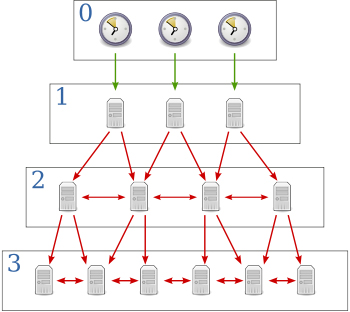
\includegraphics[scale=.4]{ntp.jpg}
	\caption{Sistemul ierarhic al protocolului NTP. Pe nivelul 0 se afl'a ceasuri atomice, GPS sau radio conectate local la calculatoarele de pe nivelul 1; pe nivelul 1 se g'asesc servere numite \emph{time servers}; pe nivelul 2 se g'asesc servere care trimit cereri NTP la nivelul 1; se poate ajunge p'jn'a la 16 nivele.}
	\label{ntpprotocol}
\end{figure}

O utilizare adi'tional'a a marcajelor temporale(\emph{timestamps}) exacte se gase'ste 'si 'in protocoalele criptografice; anumite vulnerabilit'a'ti pot fi 'inl'aturate dac'a ne putem baza pe ceasuri cu o acurate'te foarte bun'a. Fi'sierele raport create de serviciile NTP pot, de asemenea, indica atacuri care au avut loc. Crackerii obi'snuiesc s'a schimbe marcajele temporale ale fi'sierelor pentru a 'indep'arta dovezi ale activit'a'tilor. 'In unele cazuri, c'jnd nu pot fi schimbate marcajele temporale, vor trebui s'a schimbe timpul sistemului. Dar acest tip de fluctua'tii afecteaz'a serverele NTP care tind s'a ``se pl'jng'a'' 'in fi'sierele raport.

NTP este 'tinta diferitelor atacuri. 'In general, scopul unui astfel de atac este schimbarea conceptului de timp corect al 'tintei. Spre exemplu, 'in contextul unui protocol cu o autentificare bazat'a pe timp, dac'a se d'a 'inapoi ceasul 'tintei, se poate folosi o parol'a veche(deja interceptat'a) pentru autentificare. Pentru a preveni astfel de atacuri, noile versiuni ale NTP asigur'a autentificare pe baz'a de criptare a mesajelor.
%2.6.2 NTP

%2.6.4 Finger si Whois
\subsection{\emph{Finger} 'si \emph{Whois}}
Dou'a protocoale standard, finger 'si whois, sunt folosite, de obicei, pentru a c'auta informa'tii despre persoane. Primul poate pune probleme.

Protocolul finger poate fi folosit pentru a g'asi informa'tie despre un anumit utilizator sau un utilizator logat la un anumit sistem. Cantitatea 'si calitatea informa'tiei ob'tinute poate constitui o cauz'a de 'ingrijorare. Finger este considerat unul din cele mai periculoase sevicii deoarece este foarte folositor c'jnd vine vorba de investigarea poten'tialelor 'tinte. Poate dezv'alui informa'tii personale precum 'si alte informa'tii: data ultimei utiliz'ari a unui cont, locul de unde a fost folosit contul, etc.

Cea mai important'a dintre informa'tiile dezv'aluite de finger poate fi considerat'a coresponden'ta dintre nume 'si adresa de po'st'a electronic'a. Din acest motiv, multe site-uri nu folosesc finger. 

Protocolul whois este mult mai pu'tin periculos deoarece dezv'aluie numai informa'tie de contact.
%2.6.4 Finger si Whois
%capII 9 Alte protocoale
%CapII Slabiciunile protocoalelor TCP/IP

%CapIII Tipuri de atacuri pe internet
\chapter{Tipuri de atacuri}

%3.1
\section{Clasificare}
%www.ranum.com/security/computer_security/archives/internet-attacks.pdf
Atacurile care au loc pe Internet pot fi clasificate 'in urmatoarele categorii: \emph{inginerie social'a}, \emph{impersonare}, \emph{exploatarea defectelor software}, \emph{'incredere tranzitiv'a}, \emph{data driven(malware)}, \emph{infrastructur'a} 'si \emph{sabotarea serviciilor}. S'a analiz'am pe scurt fiecare dintre aceste clase de atacuri.

%http://en.wikipedia.org/wiki/Social_engineering_(security)
\subsubsection{Ingineria social'a}
Ingineria social'a(social engineering) este o colec'tie de tehnici folosite pentru a manipula diverse persoane 'si a le convinge s'a fac'a anumite ac'tiuni 'si s'a divulge informa'tie confiden'tial'a. De'si similar cu simpla fraud'a, termenul se aplic'a 'indeosebi 'in cazul 'siretlicurilor ce au ca scop adunarea de informa'tii sau ob'tinerea neautorizat'a a accesului la un sistem informatic 'si, 'in cele mai multe cazuri, atacatorul nu se 'intalne'ste niciodat'a fa't'a in fa't'a cu victima. Toate aceste tehnici sunt bazate pe anumite atribute ale modului 'in care oamenii iau decizii, cunoscute sub numele de distorsiuni cognitive, distorsiuni ce sunt exploatate de atacator 'in diverse feluri. Un exemplu de atac care s-ar putea 'incadra 'in aceasta categorie este urmatorul:

\begin{itemize}
	\item un utilizator prime'ste un email de la ``root'' cu con'tinutul: ``v'a rog schimba'ti parola 'in abbaba''
	\item utilizatorul crede c'a mesajul este autentic 'si schimb'a parola
	\item atacatorul se logheaza cu numele acestui utilizator la sistem
	\item atacatorul exploateaz'a bug-urile sistemului pentru a ob'tine acces complet la acesta.
\end{itemize}

\subsubsection{Impersonarea}
'In domeniul securita'tii, impersonarea se refer'a la furtul drepturilor de acces ale utilizatorilor autoriza'ti (de exemplu, \emph{furtul de parole}). Impersonarea unui sistem face parte, de asemenea, din aceast'a categorie(de exemplu un calculator se d'a drept alt calculator folosind  adresa IP sau adresa MAC a acestuia). Iat'a un posibil scenariu de acest tip: 

\begin{itemize}
	\item utilizatorul se conecteaz'a la re'tea prin telnet de la un terminal
	\item atacatorul, care are 'in posesie un sniffer, captureaz'a 'intreaga sesiune de logare
	\item peste un anumit timp, atacatorul se logheaza la sistem folosind id-ul de utilizator 'si parola furate.
\end{itemize}

%http://en.wikipedia.org/wiki/Exploit_(computer_security)
\subsubsection{Exploatarea defectelor}
Exploatarea defectelor se refer'a la profitarea de pe urma bug-urilor aplica'tiilor 'si sistemului de operare. \emph{Exploatatorii(exploits)} sunt buc'a'ti de software sau secven't'e de date sau comenzi care exploateaz'a un defect sau o vulnerabilitate cu scopul de a cauza manifest'ari neprev'azute sau neinten'tionate 'intr-un sistem software sau hardware('in general, computerizat). Aceste urmari pot fi de mai multe tipuri: ob'tinerea accesului la o anumit'a resurs'a privat'a, cauzarea unui atatc de sabotare a serviciilor, etc. Exploatatorii sunt clasifica'ti 'in mod normal dup'a trei criterii: tipul de vulnerabilitate pe care il exploateaz'a, modul de contact al aplica'tiei vulnerabile(local sau la distan't'a) 'si rezultatul rul'arii.

\subsubsection{'Incredere tranzitiv'a}
Atacurile care intr'a 'in categoria 'increderii tranzitive sunt acele atacuri care exploateaz'a una din propriet'a'tile rela'tiei de 'incredere dintre entit'a'ti(gazde sau re'tele), 'si anume tranzitivitatea. Proprietatea de tranzitivitate poate fi exprimat'a astfel: dac'a A are 'incredere 'in B 'si B are 'incredere 'in C, atunci A are 'incredere 'in C. De'si tranzitivitatea extinde rela'tiile de 'incredere 'intre sisteme, are 'si dezavantaje: dac'a unul din sisteme este p'ac'alit de un atacator s'a aiba 'incredere in sistemul acestuia, atunci toate celelate sisteme vor avea 'incredere 'in sistemul atacatorului. Iat'a un scenariu care ilustreaz'a acest tip de atac:

\begin{itemize}
	\item o re'tea de sta'tii de lucru partajeaz'a resurse via NFS
	\item atacatorul compromite contul de administrator de pe una din sta'tiile de lucru client
	\item atacatorul poate crea executabile privilegiate pe sistemul de fi'siere exportat de la server
	\item atacatorul creaz'a executabile privilegiate pe server 'si apoi se logheaza ca utilizator normal
	\item atacatorul execut'a programele privilegiate 'si ob'tine acces la server
\end{itemize}

%http://en.wikipedia.org/wiki/Malware
\subsubsection{Data driven / malware}
Atacurile de tip ``data driven'' folosesc diferite aplica'tii malitioase denumite ``malware'' pentru a facilita compromiterea 'tintei. Malware este denumirea pentru software-ul construit pentru a se infiltra sau a avaria un calculator. Este un termen general folosit 'in informatic'a pentru a desemna o varietate de programe ostile, intruzive 'si ``enervante''. Majoritatea utilizatorilor nu sunt 'ins'a familiari cu acest termen 'si folosesc 'in locul acestuia termenul ``virus'' 'in mod incorect pentru a descrie diferite tipuri de malware, de'si nu toate tipurile de malware sunt viru'si.

Programele sunt considerate mali'tioase pe baza inten'tiei(percepute de ceilal'ti) creatorului(nu pe baza caracteristicilor particulare). Urmatoarele tipuri de programe sunt considerate malware: viru'sii, viermii, troienii, majoritatea rootkit-urilor, spyware-ul, adware-ul, 'si alte tipuri de aplica'tii mali'tioase sau nedorite. 

Principala cale de infestare cu astfel de programe o reprezint'a Internetul, 'in special serviciile de mail 'si Web.

Exemplu:

\begin{itemize}
	\item atacatorul trimite un mail victimei cu un ata'sament un fi'sier postscript(.ps) care con'tine opera'tii cu fi'siere
	\item victima deschide ata'samentul cu un interpretor de postscript
	\item interpretorul execut'a opera'tiile din sript care adaug'a adresa gazdei atacatorului in fi'sierul ``.rhosts'' al victimei
	\item atacatorul se logheaza la gazda victim'a
\end{itemize}


%http://www.isc.org/index.pl?/ops/ds/host-count-history.php
\subsubsection{Infrastructur'a}
Atacurile din aceasta clas'a exploateaz'a sl'abiciunile protocoalelor folosite 'in Internet. Pe timpul c'jnd majoritatea acestor protocoale au fost construite, securitatea nu reprezenta o problema de luat 'in calcul, a'sa c'a nu s'a pus accentul pe aceast'a latur'a. Odata cu dezvoltarea exploziv'a a Internetului, nevoia de securitate a crescut. Dificultatea const'a 'in modificarea sau 'inlocuirea acestor protocoale cu alte protocoale securizate din cauza m'arimii imense a re'telei(la 'inceputul lui 2008 existau 'in jur de 541,677,360 de gazde conectate la Internet, comparativ cu 29,670,000 'in 1998 'si 33,000 'in 1988). 

Un exemplu de atac ce se poate 'incadra 'in aceasta categorie este ``DNS Spoofing'':

\begin{itemize}
	\item atacatorul compromite un sistem care este server de nume al unei re'tele
	\item victima are in fi'sierul ``.rhosts'' o intrare cu gazda ``foo.victimdomain.com''
	\item atacatorul adauga 'in baza de date a serverului DNS o mapare a unui dintre sistemele lui cu ``foo.victimdomain.com''
	\item atacatorul folose'ste rlogin pentru a ob'tine accesul
\end{itemize}

%http://en.wikipedia.org/wiki/Denial_of_service
\subsubsection{Sabotarea serviciilor}
Un atac de sabotare a serviciilor este o 'incercare de a face o resurs'a de pe un calculator nedisponibil'a utilizatorilor. De'si mijloacele, motivele 'si 'tintele unui atac DoS(Denial-of-service) pot varia, 'in general acesta consist'a din eforturile malevolente ale unei persoane sau grup de persoane pentru a 'impiedica buna func'tionare a unui site Web sau a unui serviciu, temporar sau pe un timp nedeterminat. F'apta'sii atacurilor de acest tip de obicei atac'a site-uri sau servicii g'azduite pe servere importante cum ar fi sisteme bancare, sisteme gateway pentru pla'ti cu cardul 'si chiar servere de nume pentru domeniile r'ad'acina. Una dintre metodele comune de atac implic'a bombardarea victimei cu cereri externe de comunicare. Atacurile DoS sunt implementate 'intr-unul din urmatoarele trei moduri: for'tarea rebotarii sistemului 'tint'a, consumarea resurselor sistemului 'tint'a p'jn'a ce acesta nu mai poate face fa't'a cererilor 'si nu mai poate asigura serviciile sau blocarea c'ailor de comunicare dintre utilizatori 'si victim'a.

Exemplu:
\begin{itemize}
	\item atacatorul bombardeaz'a cu pachete ICMP router-ul re'telei sau
	\item atacatorul bombardeaz'a cu pachete ICMP router-ul ISP-ului re'telei
\end{itemize} 


Aceasta este o clasificare teoretica a atacurilor ce pot avea loc pe Internet. 'In realitate majoritatea atacurilor intr'a 'in mai multe dintre categoriile de mai sus. De exemplu, bombardarea cu pachete ICMP a ruter-ului unei re'tele este un atac de sabotare a serviciilor care se foloseste de sl'abiciuni de infrastructur'a ale internetului, a'sadar poate fi 'incadrat 'si 'in categoria atacurilor de infrastructur'a. Viermele \emph{Code red} exploata o vulnerabilitate a sofware-ului distribuit cu Microsoft IIS(Internet Information Services) pentru a se r'aspandi 'si dup'a un anumit num'ar de zile lanse'a atacuri distribuite de sabotare a serviciilor asupra c'jtorva servere Web, printe care 'si serverul Casei Albe; deci atacul poate fi 'incadrat 'in cel pu'tin trei dintre categoriile de mai sus: malware, exploatarea defectelor 'si sabotarea serviciilor.

'In continuare voi trata c'jteva tipuri de atacuri 'in detaliu.
%3.1

%3.2
%http://www.cs.cmu.edu/~mihaib/articole/tcp/tcp-html.html
%http://www.cs.washington.edu/homes/savage/papers/CCR99.ps
\section{Colaborare 'si concuren't'a 'in Internet}
TCP este un protocol simetric(full-duplex), 'in care ambele capete pot transmite date. E mai simplu 'ins'a sa studiem problema ca si cum unul dintre participan'ti doar trimite date, iar celalalt doar le recep'tioneaz'a.

Iat'a patru diagrame(figurile \ref{com1}, \ref{com2}, \ref{com3} 'si \ref{com4})  care ilustreaz'a modul cum are loc o comunicare la nivelul TCP.

\begin{figure}[ht]
	\centering
	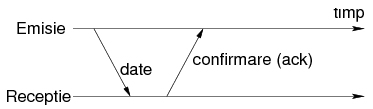
\includegraphics[scale=.7]{tcp_com_1.jpg}
	\caption{Schimbul de mesaje 'intre emi'tator si receptor. Timpul este simbolizat de sage'tile orizontale si curge spre dreapta. Sagetile oblice indic'a ``traiectoria'' pachetelor 'intre emisie si receptie. Acest desen indic'a o conversa'tie tipic'a, 'in care un pachet de date este trimis de emi'tator 'si o confirmare sose'ste apoi de la receptor. Vom prescurta pachetele de confirmare cu abrevierea standard, ACK(acknowledgement).}
	\label{com1}
\end{figure}

\begin{figure}[ht]
	\centering
	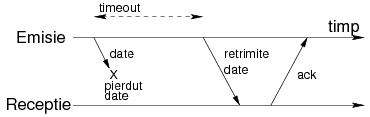
\includegraphics[scale=.7]{tcp_com_2.jpg}
	\caption{Dac'a datele sunt pierdute de protocolul IP, procotolul TCP re-transmite dupa un anumit timp pachetul care nu a fost confirmat. 'In clipa 'in care prime'ste confirmarea, 'stie c'a pachetul a ajuns la destina'tie.}
	\label{com2}
\end{figure}

\begin{figure}[ht]
	\centering
	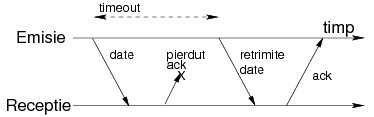
\includegraphics[scale=.7]{tcp_com_3.jpg}
	\caption{Dac'a confirmarea este pierduta de protocolul IP, procotolul TCP re-transmite dup'a un anumit timp pachetul care nu a fost confirmat. Retransmi't'ind datele nu facem dec'it o oarecare risipa; dar pentru c'a emi'tatorul nu poate distinge nicicum 'intre pierderea datelor si a confirmarii, nu are nici o alta alternativa.}
	\label{com3}
\end{figure}

\begin{figure}[ht]
	\centering
	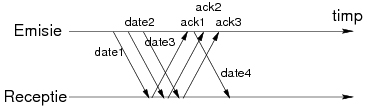
\includegraphics[scale=.7]{tcp_com_4.jpg}
	\caption{Pentru a nu irosi resursele re'telei, TCP de obicei trimite mai multe pachete 'inainte de a primi confirmarea primului. Aceasta figur'a ilustreaza o fereastr'a de emisie de dimensiune 3: TCP trimite trei pachete, 'si trimite apoi pachete noi doar daca primeste confirmari pentru cele trimise.}
	\label{com4}
\end{figure}

%3.2.1
\subsection{Controlul congestiei}
Congestia este foarte important'a, pentru ca toate cele trei atacuri discutate 'in continuare manipuleaz'a slabiciuni 'in specificarea 'si implementarea schemei prin intermediul careia TCP face fa't'a acestui fenomen. 

Asump'tia de baz'a a TCP este c'a re'teaua de transmisiune este inerent fiabil'a. TCP presupune c'a singura cauz'a de pierderi 'in re'tea este congestia. 

\paragraph{Ce este congestia?} S'a ne imagin'am un router 'in re'tea, care are trei interfe'te de 1 megabit/secunda. S'a ne imagin'am c'a pe dou'a dintre interfe'te se afl'a ni'ste trimi'tatori care emit cu 800 kbps, iar pe a treia se afl'a receptorul datelor. Suma celor doua fluxuri de 800 kbps dep'a'se'ste capacitatea leg'aturii spre receptor. Ca atare, pachetele care intr'a 'in ruter nu pot ie'si toate 'in timp util. Ruterul va trebui s'a stocheze pachetele 'in exces 'in memoria intern'a. Dar dac'a aceast'a situa'tie dureaza destul de mult, ruterul trebuie sa consume c'jte 600 kbps de memorie pentru a stoca aceste pachete 'in exces. Dupa 30 de secunde de trafic ne'intrerupt, e nevoie de peste 2Mb de RAM. Atunci c'jnd memoria router-ului este complet utilizat'a, acesta nu mai are nimic de f'acut dec'jt s'a renun'te la a mai trimite pachetele spre iesire(pur 'si simplu sunt 'sterse din memorie). Aceasta este congestia, 'si rezultatul ei, pierderea de pachete. 

TCP 'isi imagineaza c'a atunci c'jnd un pachet nu este confirmat 'in timp util, s-a pierdut fie pachetul fie confirmarea, deci re'teaua este congestionat'a. Ca atare, trimi'tatorul imediat reduce rata de transmisiune, pentru a reduce numarul de pachete din re'tea. 

Dac'a to'ti transmi'tatorii care detecteaza congestie reduc rata simultan, efectul este c'a router-ele din re'tea primesc mai putine date la intrare, 'si au timp s'a goleasc'a pachetele stocate 'in memorie trimi't'jndu-le la destina'tie. Pentru c'a marea majoritate a calculatoarelor din re'tea folosesc protocolul TCP, acest comportament duce la disparitia congestiei. 

Cum reduce emitatorul TCP rata de transmisiune? 'intr-un mod foarte simplu: reduce automat dimensiunea ferestrei, 'si mare'ste dimensiunea duratei de timeout. 'in felul acesta va face ca mai putine pachete s'a se afle simultan 'in re'tea.

%vezi ccr99.ps pag 2
%3.2.1

%3.2.2
\subsection{Spectrul participan'tilor}
Am v'azut p'jna acum care sunt mecanismele prin care TCP 'isi 'indepline'ste misiunile(unele dintre ele). Pentru a 'intelege de ce aceste mecanisme nu sunt suficiente pentru orice scenariu, trebuie s'a arunc'am o privire asupra participan'tilor la trafic din Internet 'si asupra intereselor lor contradictorii.

\emph{Stefan Savage}, un cercet'ator in domeniul informaticii, 'in special al securita'tii re'telelor, a prezentat grada'tia din figura \ref{spectru}.

\begin{figure}[ht]
	\centering
	
\includegraphics[scale=.7]{spectru.jpg}
	\caption{Inten'tiile participan'tilor la comunica'tie 'in Internet variaza 'intre dorinta de colaborare reciproc'a 'si inten'tii distructive. Proiectan'tii Internet-ului au crezut c'a utilizatorii se vor plasa doar 'in regiunea ``cooperarii''; situatia de ast'azi este 'insa net diferit'a.}
	\label{spectru}
\end{figure}

S'a analiz'am pe scurt cele patru categirii.
	
\paragraph{Cooperare:} 'in continuare multe calculatoare din Internet coopereaza pentru bunaa func'tionare a retelei. De exemplu, toate router-ele comunica 'intre ele informatii despre structura re'telei, ceea ce permite datelor s'a circule 'intre oricare doua puncte, chiar daca ele apartin unor domenii administrative distincte. 

\paragraph{Indiferen't'a:} probabil rela'tia cea mai frecvent'a 'intre doua puncte terminale din Internet este cea de indiferen't'a. De exemplu, un server Web este indiferent la ac'tiunile unei gazde, mai pu'tin dac'a aceasta vrea sa obtin'a exact ceea ce el serveste.

\paragraph{Concuren't'a:} pe de alta parte 'intre oricare dou'a calculatoare care acceseaza acela'si server de Web este o relatie de concuren't'a; dac'a serverul ar consacra primului calculator toate resursele, atunci acesta ar primi un raspuns mult mai rapid 'si mai prompt. (Nu e vorba de concuren't'a 'in sens economic, ci de competi'tie pentru resurse limitate ale re'telei.) 

\paragraph{Du'sm'anie:} Internetul permite atacuri pe scar'a larg'a 'impotriva calculatoarelor conectate, de la intruziuni, furt de informa'tie(care 'tin mai putin de natura re'telei c'jt de implementarea sau administrarea defectuoasa a programelor), p'jna la atacuri de sabotare de servicii, care pot interzice accesul la anumite servicii.

'In continuare vom analiza trei atacuri care intr'a in categoria concuren't'a.
%3.2.2

%3.2.3
\subsection{Trei atacuri asupra TCP}
Cei care ar putea face rau foarte u'sor(cei care trimit multe date, serverele) nu pot fi necinsti'ti, pentru ca-'si fac rau lor 'in'sile, iar clien'tii nu pot face rau, pentru c'a ei nu transmit multe date, ci doar recep'tioneaz'a. 

'In realitate clien'tii au la dispozi'tie o unealt'a foarte puternic'a cu care pot controla comportarea serverului fara voia acestuia: confirm'arile. 

Stefan Savage 'impreun'a cu colegii din grupul lui de cercetare au demonstrat acest lucru ``pe viu'': au luat un client Linux 'si au f'acut modificari minore 'in implementarea protocolului TCP(sub 100 de linii de cod pentru toate atacurile prezentate la un loc). Apoi au demonstrat cum acest client, folosit pentru a extrage date de la mai multe site-uri de Web foarte importante(deci care nu pot fi suspectate de colaborare), poate monopoliza re'teaua 'in detrimentul celorlalti clien'ti. 

Iat'a pe scurt trei modific'ari diferite 'si impactul fiec'areia dintre ele.

%1
\subsubsection{Diviziunea confirm'arilor}
'In TCP datele transmise formeaza un flux(stream). Fiecare pachet trimite o parte din date, 'si indic'a pozi'tionarea lor 'in flux. De pild'a, primul pachet ar putea trimite datele de la 0 la 1000, al doilea de la 1001 la 2000, etc. Confirm'arile pe de alt'a parte sunt cumulative: o confirmare care spune ``3001'' 'inseamna: ``am primit toate datele 'intre 0 si 3000; a'stept date 'incep'jnd de la 3001 'in continuare''. 'In felul acesta, dac'a o confirmare pentru un pachet se pierde(de exemplu cea pentru pachetul 1001-2000), confirmarile ulterioare o pot subsuma, reduc'jnd traficul necesar. 

Primul atac e surprinzator de simplu: c'jnd receptorul prime'ste un pachet, sa zicem cu datele 0-1000, el va trimite 'in loc de o confirmare, trei: una pentru 333, una pentru 667, una pentru 1000. Atacul este ilustrat de figura \ref{diviz1}.

\begin{figure}[ht]
	\centering
	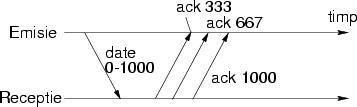
\includegraphics[scale=.7]{diviz_1.jpg}
	\caption{Atacul prin diviziunea confirm'arilor. Receptorul prime'ste un singur pachet, dar confirm'a mai multe buc'a'tele.}
	\label{diviz1}
\end{figure}

E clar c'a 'in felul acesta protocolul ram'jne corect. Problema este 'in modul 'in care emi'tatorul trebuie s'a reac'tioneze la astfel de mesaje: dac'a citim 'in RFC 2581 vom vedea un paragraf care spune urmatoarele: c'jnd un pachet de confirmare este primit, trimitatorul mare'ste fereastra cu SMSS(Sender Maximum Segment Size).

Nu ne intereseaz'a prea tare c'jt e valoarea lui SMSS(aceasta valoare este stabilita 'intre cele doua par'ti c'jnd se stabile'ste conexiunea); important e c'a, trimi't'jnd mai multe confirm'ari, receptorul poate m'ari fereastra emi't'atorului aproape 'in mod arbitrar. Dac'a alege sa confirme fiecare octet, poate mari fereastra de mii de ori dupa un singur pachet primit. Figura \ref{diviz2} arat'a ce se 'int'jmpl'a dup'a aceea.

\begin{figure}[ht]
	\centering
	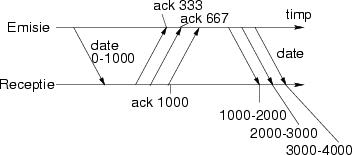
\includegraphics[scale=.7]{diviz_2.jpg}
	\caption{Rezultatul atacului prin diviziunea confirmarii. Emi'tatorul cre'ste fereastra cu o cantitate mare(SMSS) pentru fiecare confirmare primit'a, trimit'jnd o rafal'a de date imediat dupa primirea confirm'arilor.}
	\label{diviz2}
\end{figure}

Asta 'inseamn'a c'a emi'tatorul(serverul) va trimite apoi o rafal'a de pachete de date. Se observ'a c'a pachetele sunt trimise unul dupa altul, 'inainte de a da o 'sans'a re'telei s'a trimita semnale de congestie. 'In mod normal fereastra emi'tatorului cre'ste treptat p'jna atinge o valoare de echilibru, care nu produce congestie(aceasta cre'stere se numeste ``slow start''). Graficul din figura \ref{divizgraf} arat'a c'a receptorul poate primi de la surs'a documente uria'se aproape instantaneu.

\begin{figure}[ht]
	\centering
	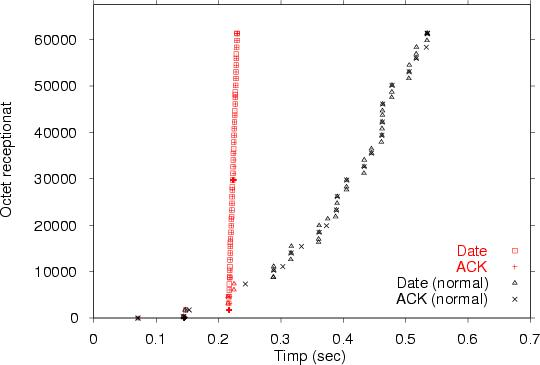
\includegraphics[scale=.7]{diviz_graf.jpg}
	\caption{Rata de transfer m'asurat'a la client 'in Internet pentru doua scheme: TCP normal si TCP modificat cu diviziunea confirm'arii. TCP-ul care tri'seaz'a obtine o rata de transfer uria'sa, 'in detrimentul celorlalte calculatoare din re'tea.}
	\label{divizgraf}
\end{figure}

%2
\subsubsection{Confirm'ari duplicate}
A doua schem'a este 'si mai simpla 'si se bazeaz'a pe aceea'si sl'abiciune din specifica'tia TCP. 'In loc s'a trimit'a mai multe pachete de confirmare diferite, receptorul trimite 'in mod repetat un singur pachet de confirmare. Receptorul poate folosi chiar pachetul de confirmare pentru octetul 1(ca 'si cum n-ar fi primit 'inca nimic). 

Figura \ref{dupl} arat'a cum se comporta emi'tatorul. Performan'ta m'asurat'a 'in Internet(si nu 'intr-o retea de laborator) este aceea'si ca pentru schema cu diviziune. 

Aceast'a schem'a este 'si mai perfida dec'jt cea precedent'a; dac'a pentru cea precedent'a serverul ar putea s'a devin'a suspicios, pentru c'a sunt confirmate doar fragmente de pachet(re'teaua are dreptul s'a fragmenteze pachetele 'in bucati, dar acest lucru se 'int'jmpl'a foarte rar, pentru c'a adesea p'ar'tile aleg o m'arime de pachet suficient de mic'a pentru a nu fi nevoie s'a fie vreodat'a fragmentat'a, din motive de performan't'a). Din punct de vedere al serverului un scenariu 'in care vin mai multe confirmari identice este perfect plauzibil(protocolul IP nu promite ca nu duplic'a pachete).

\begin{figure}[ht]
	\centering
	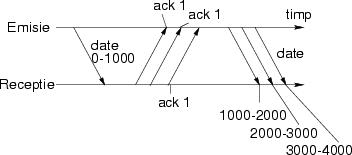
\includegraphics[scale=.7]{dupl.jpg}
	\caption{Rezultatul atacului prin duplicarea confirm'arilor. Receptorul trimite mai multe confirm'ari identice; fiecare mare'ste mult fereastra emi'tatorului, care emite apoi mai multe date.}
	\label{dupl}
\end{figure}

%3
\subsubsection{Confirm'ari anticipate}
Ultimul atac este mai riscant, deoarece confirm'a date care 'inc'a nu au fost primite. Ideea este c'a confirm'arile 'si datele se 'incruci'seaz'a pe parcurs, 'si serverul are impresia c'a datele au ajuns mult mai repede. Figura \ref{anticip} arat'a cum func'tioneaz'a acest atac.

\begin{figure}[ht]
	\centering
	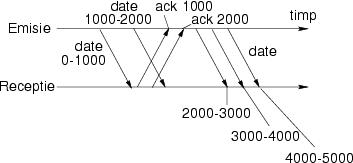
\includegraphics[scale=.7]{anticip.jpg}
	\caption{Rezultatul atacului prin anticiparea confirm'arilor. Receptorul trimite confirm'ari chiar pentru pachetele care nu au fost primite; aceste pachete rapid primite dau impresia c'a receptorul este foarte ``aproape'', 'si, ca atare, cauzeaz'a cre'sterea rapid'a a ferestrei.}
	\label{anticip}
\end{figure}

Desigur, 'in cazul unei pierderi reale de date, receptorul are probleme, pentru c'a emi'tatorul nu va re-trimite datele deja confirmate. Dar, a'sa cum arat'a cercetatorii de la Universitatea Washington, protocolul HTTP, prin care clientul comunic'a cu serverul de web, permite clientului s'a re-cear'a date de la server 'in mod selectiv. Deci pierderile la nivel TCP pot fi compensate de un client modificat prin nivele superioare de corec'tie a erorilor. 

Performan'tele schemei cu anticipare de confirmari sunt mai pu'tin spectaculoase, dar oricum, mult superioare celei a unui client normal(figura \ref{anticipgraf}).

\begin{figure}[ht]
	\centering
	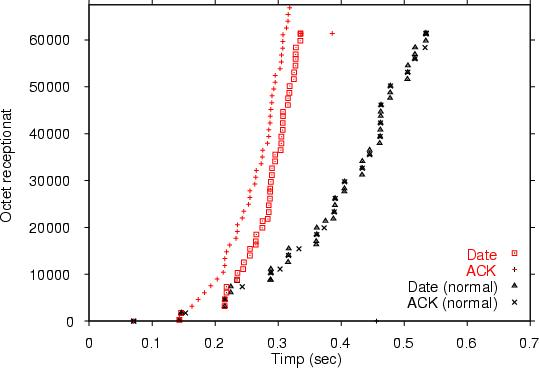
\includegraphics[scale=.7]{anticip_graf.jpg}
	\caption{Performan'ta comparat'a masurat'a 'in Internet a unui client normal 'si a unui client care foloseste schema cu confirm'ari anticipate.}
	\label{anticipgraf}
\end{figure}
%3.2.3
%3.2

%3.3
\section{Furtul de parole}
Cea mai u'soar'a cale de a p'atrunde 'intr-un sistem este de obicei pe ``u'sa din fa't'a'', adic'a prin comanda login. 'In majoritatea sistemelor, o autentificare cu succes este bazat'a pe introducerea unei parole corecte dintr-un num'ar rezonabil de 'incerc'ari.

De'si greu de crezut, au existat sisteme care stocau parolele nemodificate prin metode criptografice 'intr-un fi'sier. 'Intr-un asemenea sistem securitatea era bazat'a pe 'tinerea secret'a a numelui fi'sierului (comanda de listat con'tinutul unui director nu afi'sa numele acestui fi'sier dar putea fi accesat de oricine ii 'stia numele). Aceast'a abordare se bazeaz'a pe \emph{securitatea prin obscuritate}. Obscuritatea nu e o unealt'a de securitate proast'a, de'si a c'ap'atat o reputa'tie nu prea bun'a in acest domeniu. P'jn'a la urm'a, ce este o cheie criptografic'a dec'jt o mic'a bucat'a de obscuritate. Neajunsul aici a fost sl'abiciunea obscurita'tii 'si lipsa altor nivele de protec'tie.

Bug-urile sistemului reprezint'a un mod interesant prin care acesta poate fi ``spart'', dar nu este cel mai u'sor mod de atac. Aceast'a onoare este rezervat'a pentru parole. Un mare procentaj de penetr'ari de sistem au drept cauz'a e'secul mecanismului de parole.

Exist'a mai multe posibile cauze ale acestui e'sec. Cea mai comun'a este reprezentat'a de faptul c'a utilizatorii tind s'a aleag'a parole ``proaste''. Studii repetate au ar'atat c'a ghicirea parolelor este destul de probabil'a. Nu toat'a lumea alege parole ``slabe'', 'ins'a un atacator are nevoie, de obicei, doar de o singur'a alegere proast'a.

Atacurile prin ghicirea parolelor au trei forme. Prima implic'a 'incerc'ari de log-are folosind nume de utilizatori cunoscute 'si parole ghicite(\emph{for't'a brut'a}). Aceste 'incerc'ari se soldeaz'a cu succes uluitor de des; site-urile au de obicei perechi utilizator-parol'a de genul ``field-service'' sau ``guest-guest''. Odat'a ce atacatorul a p'atruns, principala linie defensiv'a este trecut'a; pu'tine sisteme de operare pot rezista atacurilor din interior.

Aceast'a metod'a nu ar trebui s'a fie posibil'a! Utilizatorilor nu ar trebui s'a li se permit'a un num'ar nedeterminat de 'incerc'ari de autentificare cu parole gre'site; 'incerc'arile e'suate ar trebui scrise 'in fi'siere raport, utilizatorii ar trebui s'a fie 'in'stiin'ta'ti de 'incerc'ari e'suate de log-are la conturile lor, etc. Nici unul din acestea nu este un lucru nou, dar sunt destul de rar implementate 'si rar implementate corect. Multe programe nu raporteaz'a 'incerc'ari de log-are iar fi'sierele raport ale programelor care fac acest lucru, nu sunt citite de administratori 'in mod regulat. 

Al doilea mod in care atacatorii ghicesc parolele este prin 'incercarea parolelor unui sistem 'si la alte sisteme 'si se nume'ste \emph{atac cu dic'tionar}. Acest atac are de obicei succes pentru c'a utilizatorii tind s'a refoloseasc'a parolele. Aceste parole pot fi furate de la un sistem deja compromis, sau pot fi ob'tinute de la un calculator nepenetrat 'inc'a.

A treia modalitate este de a 'inregistra o sesiune 'si a memora parola folosit'a, folosind, eventual, un sniffer. 'In cazul acestei metode nu conteaz'a c'jt de bun'a este parola, sistemul va fi compromis.

\subsubsection{C'jt de lung'a ar trebui s'a fie o parol'a?}
S-a c'azut de acord c'a vechea limit'a de opt caractere a parolei pe sistemele Unix este inadecvat'a. Dar c'jt de lung'a ar trebui s'a fie aceasta?

Una din problemele algoritmului de ``\emph{password-hashing}'' a sistemului Unix este ca folose'ste cei 'sapte bi'ti semnificativi ai fiec'arui caracter introdus drept cheie de criptare. Acest lucru este 'ins'a un efect, pentru c'a algoritmul de criptare(DES) folosit permite numai chei de 56 de bi'ti.

Cele 128 de combina'tii posibile de c'jte 'sapte bi'ti nu sunt egal probabile. Nu numai c'a majoritatea oamenilor evit'a sa foloseasc'a caractere control in parolele lor, dar majoritatea nu folosesc dec'jt litere din alfabet. De fapt tendin'ta este s'a se foloseasc'a doar minuscule(lowercase).

Putem caracteriza adev'arata valoare a parolelor folosind \emph{teoria informa'tiei}. Pentru texte normale de opt litere 'in limba englez'a, con'tinutul de informa'tie este de 2,3 bi'ti pe liter'a, poate chiar mai pu'tin. Ca urmare ram'jnem cu o cheie de aproximativ 19 bi'ti, nu 56, pentru parole compuse din cuvinte engleze'sti.

Unii utilizatori aleg nume drept parole. Acest lucru are rezultate 'si mai proaste din cauza frecven'tei anumitor nume. Experimente folosind cartea de telefoane AT\&T online au ar'atat ca un prenume con'tine numai 7,8 bi'ti de informa'tie. Acestea tipuri de parole reprezint'a o alegere foarte proast'a.

Frazele mai lungi au un con'tinut 'si mai mic de informa'tie per liter'a: 1,2 p'jn'a la 1,5 bi'ti. A'sadar, o parola de 16 octe'ti nu e asa de puternic'a precum s-ar crede dac'a este o fraz'a cu 'inteles: 19 - 24 bi'ti de informa'tie. Situa'tia este 'imbun'at'a'tit'a dac'a utilizatorul alege cuvinte independente: aproximativ 38 de bi'ti. 

Putem s'a tragem mai multe concluzii din aceste statistici. Prima, desigur, este c'a ``educa'tia'' utilizatorului in ceea ce prive'ste alegerea parolelor este vitala. Din p'acate, de'si a trecut destul timp dec'jnd acest lucru a fost semnalat, obi'snuin'tele utilizatorilor nu s-au schimbat. Au existat destule 'incerc'ari de a-i for'ta pe utilizatori s'a aleaga parole greu de ghicit, dar nu s-au soldat cu prea mult succes. E nevoie doar de un singur cont pentru a p'atrunde 'intr-o gazd'a 'si atacatori cu dic'tionare mici au rate de succes de 20\%. Dic'tionarele mari pot atinge zeci de megaocte'ti, pot include cuvinte din mai multe limbi, informa'tii personale cum ar fi num'arul de telefon, hobbie-uri, autori favori'ti, etc. O parte din aceast'a informa'tie se poate g'asi chiar in fi'sierele cu parole, restul pot fi ob'tinute cu ajutorul comenzii finger.

Scopul principal al multor atacuri asupra re'telelor nu este reprezentat at'jt de spargerea propriu-zis'a a sistemului(care este de obicei mai dificil'a), c'jt de ob'tinerea unui fi'sier cu parole. Serviciile care au fost folosite pentru sustragerea de fi'siere cu parole includ: FTP, TFTP, sistemul de mail, NIS, rsh, finger, X11, etc. Cu alte cuvinte, este un lucru u'sor de f'acut pentru un atacator, dac'a administratorul este neatent. M'asurile defensive includ grij'a 'si o atitudine conservativ'a fa't'a de software. Dac'a oamenii nu pot fi for'ta'ti s'a aleag'a parole greu de spart, e vital ca fi'sierul cu parole s'a fie p'astrat cu foarte mare grij'a astfel 'inc'jt s'a nu ajung'a 'in mainile inamicului. C'jteva m'asuri preventive:

\begin{itemize}
	\item configurarea cu aten'tie a mecanismelor de securitate ale serviciilor precum FTP 'si NIS
	\item restric'tionarea fi'sierelor disponibile pentru tftpd(un server de TFTP)
	\item evitarea plas'arii unei copii autentice a fi'sierului /etc/passwd 'in directorul de FTP anonim
\end{itemize}
%3.3

%3.4
\section{Inginerie social'a}
Desigur, vechile procedee deseori func'tioneaz'a cel mai bine. Parolele pot fi g'asite scrise pe h'jrtie l'ang'a un terminal sau 'in documenta'tie l'jng'a tastatur'a. Dar acest lucru implic'a acces fizic, a'sa c'a nu 'il voi lua 'in calcul. Tehnica de inginerie social'a de obicei implic'a un telefon 'si ceva impertinen't'a. Iat'a un scenariu care s-a petrecut la AT\&T:

\begin{quote}
``Sunt Ken Thompson. Cineva m-a sunat 'in leg'atur'a cu o problem'a cu comanda ls. M-a rugat s'a o repar.''

``OK. Ce trebuie s'a fac?''

``Schimb'a parola de la login-ul meu de pe terminalul t'au; a trecut ceva vreme dec'jnd am folosit-o.''

``Nici o problem'a.''
\end{quote}

Exist'a 'si alte metode cum ar fi \emph{mail-spoofing}(to spoof = a p'ac'ali) sau \emph{website-spoofing}. \emph{CERT} (Computer Emergency Readiness Team) avertizeaz'a 'in leg'atur'a cu mesajele(de obicei destinate administratorilor) care cer utilizatorilor s'a ruleze un anumit ``program de test'' care cere o parol'a.

Unii atacatori trimit mesaje de genul acesta:

\begin{quote}
	From:smb@research.att.com
	
	To:admin@research.att.com
	
	Subject:vizitator
	
	
	Avem un vizitator care vine s'apt'am'jna viitoare. Pute'ti ad'auga un cont pentru ea?
	
	Iat'a parola; folosi'ti exact linia urm'atoare.
	
	pxf:5bHD/k5k2mTTs:2403:147:Pat:/home/pat:/bin/sh
\end{quote}

Aceast'a procedur'a este gre'sit'a chiar dac'a mesajul nu ar fi fost de la un atacator. Dac'a Pat este un vizitator, nu ar trebui s'a foloseasc'a aceea'si parol'a pe care o folose'ste pe calculatorul personal. 

De cele mai multe ori, oameni bine-inten'tiona'ti dar insuficient preg'ati'ti sunt responsabili pentru propagarea atacurilor de inginerie social'a. De exemplu, cineva prime'ste un mail de la un prieten care 'il avertizeaz'a c'a programul X este un virus 'si ar trebui 'sters, 'si c'a trebuie s'a-i avertize pe to'ti din lista de adrese imediat. De cele mai multe ori este o p'ac'aleal'a, iar programul X poate fi vital pentru buna func'tionare a sistemului(sau chiar un modul ce face parte din mecanismul de securitate, 'stergerea sa l'as'jnd o gaur'a 'in securitatea sistemului). Cu toate acestea, mul'ti oameni cad prad'a acestui tip de p'ac'aleli 'si o r'asp'jndesc.

%3.4.1
%http://en.wikipedia.org/wiki/E-mail_spoofing\subsection{E-mail spoofing}
\subsection{E-mail spoofing}
Termenul ``e-mail spoofing'' este folosit pentru a descrie o activitate fraudulent'a care implic'a folosirea e-mail-ului. Const'a in trimiterea unui mesaj 'in care adresa trimi't'atorului 'si alte p'ar'ti ale antetului sunt alterate astfel 'inc'jt s'a dea impresia c'a provin de la o alt'a surs'a. Este o tehnic'a folosit'a 'in special pentru \emph{spam} 'si \emph{phishing}(impersonarea unei entit'ati de 'incredere cu scopul ob'tinerii de informa'tii cum ar fi parole, nume de utilizatori, detalii ale cardului) pentu a ascunde originile mesajului. Prin modificarea anumitor proprieta'ti ale e-mail-ului, cum ar fi c'jmpurile From, Return-Path 'si Reply-To, utilizatori r'au inten'tiona'ti 'i'si pot ascunde identitatea eventual poz'and o surs'a de 'incredere. Este asociat, de obicei, cu website spoofing.
%3.4.1

%3.4.2
%http://en.wikipedia.org/wiki/Website_spoofing
\subsection{Website spoofing}
Website spoofing reprezint'a actul de a crea un site cu inten'tia de a induce 'in eroare utilizatorii f'acandu-i s'a cread'a c'a site-ul a fost creat de o persoan'a sau o organiza'tie diferit'a. 'In mod normal acest lucru se ob'tine prin imitarea aspectului site-ului 'tint'a 'si, eventual, prin adoptarea unui URL asem'an'ator.

O alt'a tehnic'a const'a 'in folosirea unui URL ``ascuns''. Folosind \emph{redirec'tionarea URL-urilor} sau \emph{caractere de control}, adresa poate p'area valid'a 'in timp ce ascunde adresa sitului capcan'a.

Obiectivul unei astfel de proceduri poate fi fraudulent, deseori asociat cu phishing, sau poate fi criticarea sau prodierea unei persoane sau unei organizatii. De exemplu, in noiembrie 2006, dou'a astfel de site-uri au fost create; conform acestor site-uri Microsoft a cump'arat Firefox 'si a scos pe pia't'a Microsoft Firefox 2007.
%3.4.2

%3.4.3
%http://en.wikipedia.org/wiki/Cross-site_scripting
%www.linux-magazin.ro/pdf/ 04/lm_04_dec_03_091-093_crosssite.pdf
\subsection{Atacuri cross-site}
Cross-site scripting sau \emph{XSS} este un tip de vulnerabilitate 'int'jlnit'a de obicei la aplica'tiile web care permit utilizatorilor r'au inten'tiona'ti s'a injecteze cod 'in pagini care pot fi v'azute de al'ti utilizatori. Exemple de astfel de cod sunt HTML si scripturi pe partea de client. Astfel de vulnerabilit'a'ti au fost exploatate pentru a conduce la puternice atacuri de tip phishing.

Chiar dac'a pare de necrezut, un individ 'inarmat cu un banal browser poate provoca stric'aciuni mari exploat'jnd g'auri de securitate existente 'in multe aplica'tii web din ziua de azi.

\subsubsection{Furtul parolelor}
Cu pu'tin javascript 'si HTML se poate u'sor ob'tine parola unui utilizator. Iat'a un scenariu posibil.

\begin{quote}
	S'a presupunem c'a un individ vrea s'a afle parola de mail a unui anumit utilizator. Atacatorul 'stie c'a acest utilizator folose'ste o aplica'tie webmail, de exemplu \emph{webmail.exemplu.ro}. Aceast'a aplica'tie web poate primi mail in format HTML.
	
	Primul pas pe care trebuie s'a 'il fac'a atacatorul este s'a creeze o pagin'a de login care este identic'a(sau seaman'a foarte bine) celei pe care se logheaz'a utilizatorul la contul lui de pe webmail. S'a presupunem c'a atacatorul are un server propriu 'si salveaz'a pagina sub forma \emph{siteulmeu.ro/mail}. Singura diferen't'a este c'a formularul fals de login 'ii trimite lui parola 'si user-ul, dup'a care 'il redirec'tioneaz'a pe utilizator spre webmail.exemplu.ro.
	
	Am'anuntul r'amas de rezolvat este urm'atorul: cum 'il face atacatorul pe utilizator s'a se logheze de pe \emph{siteulmeu.ro/mail} 'si nu de pe \emph{webmail.exemplu.ro}. Atacatorul trimite un mail care con'tine un script 'in javascrit ce 'il redirec'tioneaz'a spre pagina \emph{siteulmeu.ro/mail}. Pentru un utilizator experimentat, poate p'area dubios, pentru c'a o aplica'tie web, odata logat, nu 'i'ti mai cere o re-logare. Majoritatea utilizatorilor, 'ins'a vor crede c'a este o defec'tiune 'si vor c'adea 'in capcan'a.
\end{quote}

\subsubsection{Link-uri ascunse}
Un alt poten'tial pericol este reprezentat de atributul SRC al tag-ului IMG. Iat'a de ce.

\begin{quote}
	Avem o aplica'tie web de tip forum 'si presupunem c'a un utilizator cu drepturi de administrator poate 'sterge toate post-urile acces'jnd link-ul \emph{exemplu.ro/forum/admin/delete.php?what=\-topics\&which=all}. Un utilizator oarecare pune un post care are la sfar'sit o etichet'a IMG care 'in mod normal afi'seaz'a o imagine. Numai c'a atacatorul a scris \emph{$<$img src=�http://exemplu.ro/\-forum/admin/delete.php?what=topics\&which=all�$>$}. C'jnd un utilizator normal, f'ar'a drepturi de administrator 'incarc'a pagina care con'tine acest post, browser-ul va face o cerere la server pentru aceast'a adresa 'si nu va ob'tine nimic. A'sadar nu va ap'area nici o imagine, dar nici alte efecte nu vor avea loc.
	
	Dezastrul are loc atunci c'jnd unul din administratori cite'ste postul. Adminsistratorul se logheaz'a. 'In acest moment are drepturi de administrator pe forum. 'Incarc'a pagina cu pricina 'si cererea c'atre server pentru ob'tinerea ``imaginii'' este f'acut'a. Efectul? Toate post-urile sunt 'sterse.
	
	Desigur, acest scenariu presupune c'a atacatoru cunoa'ste exact link-ul ce trebuie accesat pentru 'stergerea mesajelor 'si c'a odat'a apelat acest link nu va fi nevoie de confirmare, etc.
\end{quote}
%3.4.3
%3.4

%3.5
%http://en.wikipedia.org/wiki/Distributed_denial_of_service#Distributed_attack
%http://www.cs.cmu.edu/~mihaib/articole/ddos/ddos-html.html
\section{Sabotarea serviciilor}
%3.5.1
\subsection{Manifest'ari}
CERT clasific'a simtomele atacurilor de sabotare a serviciilor astfel:

\begin{itemize}
	\item performan't'a excesiv de sc'azut'a a re'telei;
	\item indisponibilitatea anumitor site-uri web;
	\item inabilitatea de a accesa orice site web;
	\item cre'sterea dramatic'a a num'arului de e-mail spam primit(``Mail-Bomb'').
\end{itemize}

Atacurile de acest tip pot cauza proble 'intr-o intreag'a re'tea, nu numai calculatorului 'tint'a. De exemplu, l'a'timea de band'a a unui router dintre Internet 'si LAN-ul 'in care se afl'a 'tinta poate fi consumat'a de un atac, compromi't'jnd 'intreaga re'tea.

Dac'a un atac are loc la o scar'a suficient de mare, 'intregi regiuni geografice pot r'am'jne f'ar'a acces la Internet, chiar f'ar'a inten'tia atacatorului.
%3.5.1

%3.5.2
\subsection{Metode de atac}
Atacurile pot fi direc'tionate c'atre orice tip de gazd'a dintr-o re'tea, incluz'jnd router-e, servere web 'si e-mail sau servere de nume.
Un atac DoS poate fi s'av'jr'sit 'in mai multe moduri. Cele cinci tipuri principale sunt:

\begin{enumerate}
	\item consumul resurselor computa'tionale precum l'a'timea de band'a, spa'tiul pe disc sau timpul procesorului;
	\item subminarea informa'tiei de configurare, cum ar fi informa'tia de rutare;
	\item subminarea informa'tiei despre stare, cum ar fi resetarea nesolicitat'a a unei sesiuni TCP;
	\item subminarea componentelor fizice ale unei re'tele;
	\item blocarea canalului de comunicare dintre victim'a 'si utilizatorii serviciilor oferite de aceasta.
\end{enumerate}

Un atac DoS poate include execu'tia unor programe mali'tioase cu diferite scopuri:

\begin{itemize}
	\item folosirea la maxim a ciclilor procesorului, 'imipiedic'jnd alte procese s'a func'tioneze adecvat;
	\item provocarea de erori care s'a impiedice buna func'tionare a sistemului;
	\item exploatarea erorilor sistemului de operare pentru a cauza epuizarea resurselor;
	\item cauzarea bloc'arii sistemului;
	\item lansarea unor atacuri iFrame DDoS, 'in care un document HTML con'tine foarte multe frame-uri ale unei pagini de pe situl 'tint'a(un atac surprinz'ator de simplu 'si destul de eficient)
\end{itemize}

%todo: ICMP floods etc
%3.5.2

%3.5.3
\subsection{Atacuri distribuite de sabotare a serviciilor}
C'jnd trimite un pachet c'atre o anumit'a destina'tie pe Internet, sursa pune 'inauntru toate informa'tiile necesare pentru a trimite pachetul 'in cealalt'a parte, inclusiv propria ei adres'a. Asta implic'a 'ins'a c'a avem ``'incredere'' 'in surs'a, c'a nu va trimite pachete malformate, 'si c'a nu va min'ti 'in ceea ce prives'te propria ei adres'a. 

'Intr-adev'ar, router-ele nu verific'a dac'a sursa unui pachet pe care 'il primesc este corect'a, 'si, 'in general, nici nu pot face a'sa ceva, pentru c'a router-ele pot primi pe aceea'si interfa't'a pachete de la zeci de milioane de adrese diferite. Unul din ingredientele care face atacurile distribuite at'jt de periculoase este chiar acest lucru: sursele pot min'ti 'in ceea ce prive'ste propria lor identitate, pun'jnd valori arbitrare 'in pachet. Aceasta tehnic'a se nume'ste 'in jargon ``spoofing'' (acest termen ar putea fi tradus prin ``escrocherie''). 

Pentru c'a, 'in general, companiile au servere foarte puternice, ele nu pot fi inundate dac'a atacul porne'ste de la un calculator obi'snuit: aceast'a nu poate genera suficient trafic, 'si adesea nu are destul'a capacitate de re'tea pentru a sufoca victima cu trafic. Atacatorii au dezvoltat scule care functioneaza 'in doua etape:

\begin{enumerate}
	\item Infiltreaz'a viru'si sau viermi 'in zeci, sute sau chiar mii de calculatoare. Tehnologiile pentru acest gen de atac sunt cunoscute de foarte mult'a vreme, chiar dinainte de existen'ta Internetului. 
	\item Calculatoarele infectate execut'a apoi un program de atac, care a'steapt'a comenzi de la distan't'a. C'jnd primesc o astfel de comand'a, toate aceste calculatoare pornesc simultan un atac concentrat asupra victimei. 
\end{enumerate}

\subsubsection{O evaluare a numarului de atacuri}
'In luna iulie 2001 a avut loc al 10-lea simpozion pentru securitate USENIX; acolo a fost prezentat un articol care 'incearc'a s'a estimeze numarul de atacuri DDoS din Internet. Cei trei autori sunt cercetatori la universitatea din California din San Diego. Stefan  Savage este unul dintre cei trei autori.

Articolul despre DDoS se bazeaz'a pe o idee foarte simpl'a 'si foarte elegant'a: dac'a pachetele de atac folosesc (spoof) adrese sursa absolut la 'int'jmplare (uniform distribuite 'intre 0 si $2^{32}-1$), atunci c'jnd sursa va 'incerca s'a raspund'a la un astfel de pachet, va trimite raspunsul unui calculator din Internet la 'int'jmplare. Acest fenomen este numit de autori ``'impra'stiere''(backscatter); o ilustratie a sa este 'in figura \ref{backscatter}.

\begin{figure}[ht]
	\centering
	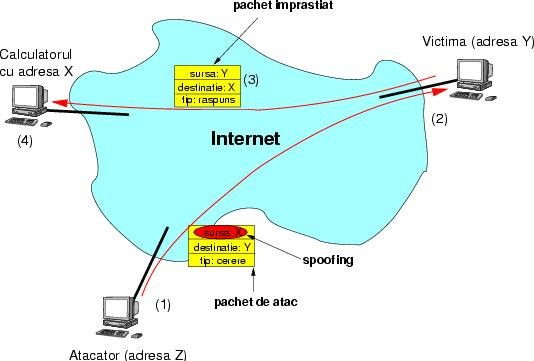
\includegraphics[scale=.6]{backscatter.jpg}
	\caption{'Impra'stierea pachetelor de raspuns la un atac. (1)Atacatorul insereaza' o adres'a surs'a arbitrar'a X 'in pachetul folosit pentru atac (2)Victima prime'ste pachetul (3)Victima r'aspunde calculatorului cu adresa X (4)Calculatorul cu adresa X primeste un pachet de raspuns din senin}
	\label{backscatter}
\end{figure}

Aceast'a observa'tie ofer'a cheia monitoriz'arii atacurilor: dac'a atacurile sunt suficient de multe ele vor putea fi observate de la orice calculator din Internet. Un calculator conectat la Internet, va primi un pachet r'aspuns, 'in medie, la fiecare $2^{32}$ pachete de atac (aproximativ patru miliarde).

Asump'tia c'a adresele sunt generate la 'int'jmplare este foarte important'a pentru a putea face o estimare statistic'a corect'a; autorii au investigat toate pachetele software disponibile public pentru atacuri distribuite, 'si 'in toate aceste programe adresa surs'a este 'intr-adevar generat'a folosind numere aleatoare cu distribu'tie uniforma (autorii au tras concluzia c'a, dac'a asump'tia de uniformitate nu e adevarata, rezultatele ob'tinute vor subestima numarul de atacuri, 'si nu 'il vor supraestima).

Autorii studiului au ob'tinut acces la un router care serve'ste o re'tea foarte mare, care contine $2^{24}$ adrese, adic'a 1/256 din num'arul total de adrese din Internet (router-ul reprezenta singura conexiune a acestei re'tele la Internet). L'jnga acest router a fost instalat un PC, programat s'a noteze informa'tii despre toate pachetele care circul'a dinspre 'si spre aceasta re'tea.

PC-ul a colectat date timp de trei sapt'am'jni, 'in trei experimente de c'jte o saptam'jn'a, la scurt timp unul dup'a altul. Datele colectate au fost apoi analizate separat, elimin'jnd traficul legitim, 'si pastr'jnd numai pachetele 'impr'a'stiate (pachete de tip r'aspuns care vin f'ar'a o cerere ini'tiat'a din interiorul re'telei). 

Datorit'a asump'tiei de distribu'tie uniform'a, aceste pachete reprezint'a, 'in medie, 1/256 din 'intregul trafic din Internet care sunt atacuri DDoS. Num'ar'jnd aceste pachete se poate ob'tine estimarea amplorii fenomenului la scar'a mondial'a.

\subsubsection{Numere 'ingrijor'atoare}
Rezultatele au fost foarte 'ingrijor'atoare: 'in cele trei s'apt'am'jni au fost observate 200 de milioane de pachete de acest gen. Acest trafic trebuie 'inmul'tit cu 256 pentru a ob'tine traficul din 'intregul Internet: 51 de miliarde de pachete! Consider'jnd c'a acest trafic este focalizat pe un num'ar relativ mic de victime, dimensiunile sunt 'infrico'satoare.

Dar pachetele captate con'tin multe alte informa'tii. De exemplu, con'tin adresele victimelor, care r'aspund la pachetele-atac. Din tipul de pachet se poate infera tipul de atac. Folosind distribu'tia pachetelor 'in timp, autorii au 'incercat s'a atribuie pachetele unor atacuri distincte 'si s'a m'asoare frecven'ta, durata 'si intensitatea atacurilor. 

S-a dedus ca au fost 12800 de atacuri 'in aceast'a perioad'a, asupra a 5000 de victime distincte. Cele mai lente atacuri au avut c'jte 50 de pachete/secund'a, iar cele mai puternice, peste 15000 de pachete/secund'a. Cel mai intens a avut peste dou'a treimi de milion de pachete/secund'a! 

Studiind solu'tiile disponibile comercial pentru a contracara atacurile de acest gen la acel moment, autorii afirmau c'a un atac de 500 de pachete/secund'a poate pune 'in genunchi un server mic, 'si c'a un firewall sofisticat poate tolera p'jna la 14000 pachete/secund'a. Ca atare, multe din atacurile observate sunt ucig'atoare pentru companii mici, 'si unele dintre ele pot fi fatale 'si pentru instala'tii deosebit de scumpe 'si sofisticate. 

Durata atacurilor este 'in medie scurt'a: 50\% din atacuri dureaz'a mai pu'tin de 10 minute, dar 2\% din atacuri dureaz'a ore, c'jteva zeci de atacuri fiind ne'intrerupte timp de mai multe zile consecutive. 

Cele mai multe victime (65\%) au suferit un singur atac, 18\% suferind dou'a atacuri. Dar unele victime au suferit multiple atacuri, uneori mai multe atacuri diferite simultan.

Cele mai multe atacuri vizeaz'a sistemul de operare 'si capacitatea lui de a procesa pachete(adic'a atacul nu e direc'tionat asupra unui anume port). Unele atacuri sunt 'ins'a directionate spre aplica'tiile care se execut'a pe calculatorul atacat, cum ar fi servere de web sau servere de chat. Un num'ar relativ mic de atacuri love'ste 'in puncte foarte importante pentru infrastructura Internetului: servere de nume si router-e. De'si aceste atacuri sunt pu'tine, impactul lor poate fi enorm, pentru c'a pot afecta toat'a por'tiunea de re'tea care depinde de serverul sau router-ul afectat. Cam 1-3\% dintre atacuri au fost de acest tip.

Pe l'jng'a aceste statistici, autorii au 'incercat s'a traduc'a adresele IP 'in nume 'si s'a fac'a o clasificare dup'a domeniul 'si 'tara acestora. Rezultatele acestui demers pot fi observate 'in figura \ref{ddosdom}.

\begin{figure}[ht]
	\centering
	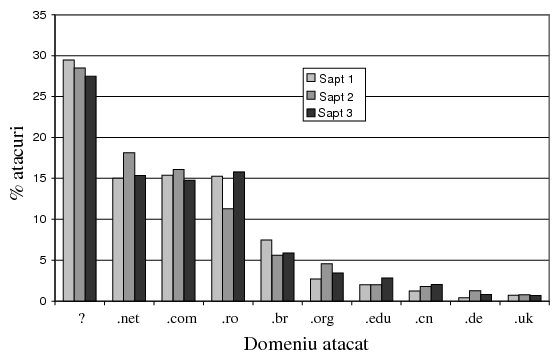
\includegraphics[scale=.6]{ddos_domain_clas.jpg}
	\caption{Procente din atacurile DDoS grupate dup'a sufixul domeniului victimei. Semnul 'intrebarii indic'a calculatoare pentru care nu a putut fi determinat numele pornind de la adresa IP.}
	\label{ddosdom}
\end{figure}

Marea surpriz'a a constat 'in faptul c'a primul domeniu din acest clasament care apar'tine unei 't'ari a fost \emph{.ro}. De asemenea, pe locul 'intai 'in lume dup'a num'arul de atacuri a fost, 'in mod surprinz'ator, un ISP din Rom'jnia, victim'a a aproximativ 5\% din totalul atacurilor din perioada monitorizat'a.
%3.5.3
%3.5

%3.6
%http://en.wikipedia.org/wiki/Malware
\section{Malware}
Conform anumitor surse, se pare c'a majoritatea programelor pentru calculator produse 'in ziua de azi sunt mali'tioase. Rezultatele publicate de compania \emph{Symantec} 'in 2008 sugereaz'a c'a ``rata producerii de cod mali'tios sau nedorit s-ar putea s'a o dep'aseasc'a pe cea aplica'tilor legitime''. De asemenea, conform companiei \emph{F-Secure}, ``At'jt de mult malware a fost produs 'in 2007 c'jt 'in ultimii 20 de ani la un loc''. Dac'a aceste afirma'tii sunt bine 'intemeiate sau sunt produsul unor ``strategii de marketing'', nu se poate 'sti cu exactitate. Oricum ar fi 'ins'a, situa'tia este destul de alarmant'a.

\subsection{Scop}
Multe dintre primele programe infec'tioase, incluz'jnd \emph{Internet Worm} 'si o parte din viru'sii pentru MS-DOS, au fost scrise ca experimente sau glume 'si inten'tionate s'a fie cel mult ``enervante''. Tinerii programatori care 'inv'a'tau despre viru'si obi'snuiau s'a scrie astfel de programe doar ca s'a dovedeasc'a faptul c'a pot face acest lucru sau s'a vad'a c'jt de mult se pot r'asp'jndi. P'jn'a 'si 'in 1999, anumi'ti viru'si care s-au r'asp'jndit foarte mult, precum \emph{virusul Melissa}, se pare c'a au fost scri'si din acelea'si motive.

Exist'a desigur 'si programe mai ostile care create pentru a vandaliza sau a produce pierderi de date. Mul'ti dintre viru'sii MS-DOS 'si viermele \emph{Windows ExploreZip}, de exemplu, au fost programa'ti s'a distrug'a fi'sierele de pe hard disk sau s'a corup'a sistemul de fi'siere. Viermele \emph{Code Red} sau viermele \emph{Ramen} cad 'in aceea'si categorie fiind programa'ti s'a vandalizeze pagini web.

Cu toate acestea, de c'jnd a avut loc explozia Internetului, majoritatea software-ului mali'tios a fost creat din motive de profit. De exemplu, 'incep'jnd cu 2003, majoritatea viru'silor 'si viermilor au fost proiecta'ti s'a preia controlul asupra calculatoarelor(asa-numitele ``calculatoare zombie'') pentru a le folosi s'a trimit'a \emph{email spam}, s'a stocheze date de contraband'a sau s'a contribuie la atacuri distribuite de sabotare a serviciilor ca o form'a de 'santaj.

O alt'a categorie de malware strict pentru profit, nou ap'arut'a, este spyware-ul. Aceste tipuri de programe sunt proiectate pentru a monitoriza obiceiurile de ``surf-are'' pe web ale utilizatorului, a'fi's'jnd reclame nesolicitate care corespund profilului acestuia. Acest tip de aplica'tii mali'tioase nu se r'asp'jndesc ca viru'sii; sunt, 'in general, instalate prin exploatarea g'aurilor de securitate, sau se afl'a in acela'si pachet de instalare cu alt program.

Chiar 'si formele de malware care se rezum'a la a se replica 'si ,poate, a-'si face cunoscut'a prezen'ta prin diferite moduri, pot crea probleme pentru utilizator. Acest lucru se 'int'jmpla deoarece ocup'a memorie ce poate fi 'intrebuin'tat'a de programele legitime, ceea ce poate duce la comport'ari nea'steptate 'si chiar la blocarea sistemului. Pe l'jng'a acest lucru, o mare parte din programele mali'tioase au bug-uri ce pot duce la consumarea resurselor sau pierderi de date, chiar dac'a f'ar'a inten'tia creatorului. Majoritatea acestor aplica'tii, 'in special spyware-ul 'si adware-ul, au un efect foarte ``enervant'': 'incetinirea sistemului.

%3.6.1
%http://en.wikipedia.org/wiki/Computer_virus
%http://en.wikipedia.org/wiki/Timeline_of_notable_computer_viruses_and_worms
%http://en.wikipedia.org/wiki/Computer_worm
\subsection{Malware infec'tios: viru'si 'si viermi}
\subsubsection{Viru'si}
Un virus de calculator este un program care se poate copia pe el 'insu'si 'si poate infecta un calculator f'ar'a permisiunea sau cuno'stin'ta tilizatorului. Virusul original poate modifica copiile, sau copiile se pot modifica singure, ca 'in cazul viru'silor polimorfici sau metamorfici, cu scopul p'ac'alirii programelor antivirus. Un virus se poate r'asp'jndi de la un calculator la altul doar c'jnd gazda sa ajunge la calculatorul neinfectat, prin diverse medii de transport(re'tea, Internet, dischet'a, CD, etc.). Se mai poate r'asp'jndi prin ifectarea sistemului de fi'siere al re'telei(de exemplu NFS) sau a unui sistem de fi'siere accesat de un alt calculator. 

Majoritatea calculatoarelor personale sunt, 'in ziua de azi, conectate la internet 'si la re'tele locale, ceea ce faciliteaz'a r'asp'jndirea codului mali'tios. Viru'sii pot profita de servicii cum ar fi World Wide Web sau e-mail, Instant Messenging 'si file shareing pentru a se r'asp'jndi 'si, ca urmare, diferen'ta dintre viru'si si viermi nu mai este atat de evident'a. Mai mult, unele surse folosesc o terminologie alternativ'a, 'in care orice form'a de malware care se auto-copiaz'a este un virus.

\paragraph{Istorie.}
Virusul \emph{Creeper} a fost detectat pentru prima oar'a 'in ARPANET la 'inceputul anilor '70. Se propaga via sistemul de operare \emph{TENEX} 'si putea folosi orice modem conectat la sistem pentru a se r'asp'jndi pe alte calculatoare. Afisa mesajul ``I'M THE CREEPER : CATCH ME IF YOU CAN.''. Se zone'ste c'a programul \emph{Reaper}, 'si el tot un virus, ap'arut la scurt'a vreme dupa Creeper, care c'auta copii ale acestuia 'si le 'stergea, a fost scris tot de creatorul lui Creeper. 

'In 1982 un program mali'tios numit \emph{Elk Cloner} a fost scris pentru sistemele Apple II de c'atre Richard Skrenta. Apple II era vulnerabil din cauza faptului c'a 'i'si stoca sistemul de operare pe dischet'a. Felul cum a fost proiectat combinat cu ignoran'ta publicului a condus la prima r'asp'jndire de scar'a larg'a a unui virus.

'In 1983 termenul ``virus'' este adoptat de Frederick Cohen pentru a descrie programele care se auto-copiaz'a. El define'ste un virus ca fiind ``un program care poate infecta alte programe mofific'jndu-le s'a includ'a o copie posibil evoluat'a a acestuia''. 

'In 1986, primul virus pentru calculatoare personale scap'a de sub control. Acesta era un virus de sector de boot-are numit (c)Brain 'si creat de fra'tii Farooq Alvi 'in Lahore, Pakistan. Fra'tii au creat virusul pentru a opri r'asp'jndirea copiilor piratate ale programelor pe care ei le scriseser'a. 

'Inainte ca re'telele de calculatoare s'a devin'a populare, majoritatea viru'silor se propagau prin intermediul dischetelor. La apari'tia calculatoarelor personale mul'ti utilizatori schimbau informa'tie 'si programe folosind dischete. Unii viru'si se r'asp'jndeau infect'jnd programe stocate pe acestea 'in timp ce altele se instalau 'in sectorul de boot cea ce asigura faptul c'a vor fi 'inc'arca'ti in memorie c'jnd utilizatorul va porni calculatorul folosind discheta.

La mijlocul anilor 1990 au ap'arut viru'sii de tip macro. Majoritatea acestor viru'si sunt scri'si 'in limbajul de scriptare ale programelor Microsoft cum ar fi Word sau Excel. Ace'sti viru'si se propag'a prin infectarea documentelor Microsoft Office. Deoarece Word 'si Excel erau disponibile 'si pentru Mac OS, majoritatea acestor viru'si au reu'sit s'a se r'asp'jndeasc'a si pe sistemele Macintosh. Majoritatea acestor viru'si nu aveau abilitatea de a trimite mail infectat. Cei care se r'asp'jndeau prin e-mail se foloseau de interfa'ta COM(Component Object Model) a Microsoft Outlook.

Unii viru'si pot trimite o adres'a web 'intr-un mesaj instant la toate contactele din lista sitemului infectat. Dac'a receptorul, crez'jnd ca link-ul este de la o surs'a de 'incredere, acceseaz'a acel website, virusul ``g'azduit'' site este capabil s'a infecteze noul calculator 'si s'a continue propagarea.

Cea mai nou'a specie a familiei de viru'si este \emph{virusul cross-site scripting}. A fost demonstrat academic 'in 2005. Acest virus utilizeaz'a vulnerabilit'a'tile de tip XSS pentru a se propaga. Cele mai notabile site-uri afectate au fost MySpace 'si Yahoo.

\paragraph{Strategii de infectare.}
Pentru a se auto-replica, unui virus trebuie s'a i se permit'a s'a execute cod 'si s'a scrie 'in memorie. Din acest motiv, mul'ti viru'si se ata'seaz'a la fi'siere executabile care pot face parte din aplica'tii legitime. Dac'a un utilizator 'incearc'a sa porneasc'a un program infectat, codul virusului poate fi executat mai 'int'ji. Viru'sii pot fi clasifica'ti 'in dou'a categorii, pe baza comport'arii la execu'tie. Viru'sii \emph{nonreziden'ti} caut'a imediat alte poten'tiale gazde, le infecteaz'a 'si apoi transfer'a controlul programului pe care l-au infectat. Viru'sii \emph{reziden'ti} nu caut'a alte gazde la rulare ci se 'incarc'a in memorie 'si transfer'a controlul programului gazd'a. Virusul r'am'jne activ 'si infecteaz'a noi gazde c'jnd fi'sierele imagine sunt accesate de alte programe sau de sistemul de operare.

\subparagraph{Viru'si nonreziden'ti} constau din dou'a module: un modul de c'autare 'si un modul de replicare. Modulul de c'autare este responsabil cu g'asirea a noi fi'siere de infectat. Pentru fiecare nou executabil g'asit, modulul de c'autare apeleaz'a modulul de replicare pentru a infecta fi'sierul.

\subparagraph{Viru'si reziden'ti} con'tin un modul de replicare similar cu cel folosit de cei nonreziden'ti. Diferen'ta este c'a acesta nu este apelat de un modul de c'autare. 'In schimb virusul 'incarc'a modulul de replicare 'in memorie c'jnd este executat 'si se asigur'a c'a acest modul este executat de fiecare dat'a c'jnd o anumit'a opera'tie ce 'tine de sistemul de operare este apelat'a. De exemplu acest modul ar putea fi apelat de fiecare dat'a c'jnd sistemul de operare execut'a un fi'sier. I'n acest mod virusul infecteaz'a fiecare program executat pe acel calculator.

\subsubsection{Viermi}
Un ``vierme'' este un program de calculator care se poate auto-replica. Folose'ste re'teaua pentru a trimite copii altor noduri(terminale ale aceleia'si re'tea), 'si poate fa'ce acest lucru f'ara interven'tia utilizatorului. Spre deosebire de un virus, nu trebuie s'a se ata'seze la alte programe. Aproape 'intotdeauna viermii provoac'a rau re'telei, chiar dac'a dor prin consumarea la'timii de band'a, 'in timp ce viru'sii aproape 'intotdeauna,k corup sau modific'a fi'sierele de pe calculatorul infectat.

Termenul de ``vierme'' a fost folosit prima data 'in romanul 'stiin'tifco-fantastic ``The Shockwave Rider'' publicat 'in 1975 de John Brunner.

Pe 2 noiembrie 1988 viermele Morris(Internet worm), creat de Robert Tappan Morris, infecteaz'a sistemele DEC VAX si Sun care rulau BSD UNIX conectate la Internet 'si devine primul vierme care s'a r'asp'jndit excesiv, 'si unul dintre primele programe care exploatez'a vulnerabilita'ti de tipul ``buffer overflow''.

Mul'ti viermi au fost crea'ti numai cu inten'tia de a se r'asp'jndi, 'si nu 'incearc'a s'a afecteze sistemele prin care trec. 'In orice caz, a'sa cum au ar'atat viermele Morris, traficul din re'tea 'si alte efecte neinten'tionate pot cauza probleme majore. O ``'inc'arc'atur'a''(``payload'') este cod proiectat s'a fac'a mai mult dec'jt s'a propage viermele. De exemplu, poate s'a 'stearg'a fi'siere de pe un sistem gaz'da sau s'a trimit'a documente prin e-mail. O ``'inc'arc'atur'a'' 'int'jlnit'a la majoritatea viermilor const'a 'in instalarea unei ``u'si''(backdoor) pe calculatorul infectat pentru a crea un calculator ``zombie'' sub controlul autorului viermelui. Re'tele alc'atuite din astfel de sisteme sunt intitulate ``botnets'', 'si sunt folosite deseori de cei care trimit spam. Spammer-i sunt considera'ti a fi o surs'a de fonduri pentru crearea a astfel de viermi. Unii autori de viermi au fost prin'si v'jnz'jnd liste de adrese IP ale sistemelor infestate spammer-ilor; al'tii 'incearc'a s'a 'santajeze companii amenin't'jndu'le cu atacuri de sabotare a serviciilor.
%3.6.1

%3.6.2
\subsection{Mascarea programelor mali'tioase: troieni, rootkit-uri 'si backdoor-uri}

\subsubsection{Troieni}
Pentru ca un program mali'tios s'a 'i'si duc'a scopul la bun sf'jr'sit, trebuie sa func'tioneze f'ar'a s'a fie oprit 'intrun fel sau altul, sau s'ters de utilizatorul sau administratorul calculatorului pe care ruleaz'a. De asemenea, mascarea poate ajuta la chiar la instalarea aplica'tiei. C'jnd un program mali'tios este deghizat 'in ceva dezirabil, utilizatorii ar putea fi tenta'ti s'a 'il instaleze f'ar'a s'a 'stie care 'ii este scopul de fapt. Aceast'a tehnic'a este folosit'a de \emph{troieni}.

'In linii mari, un troian este orice program care invit'a utilizatorul s'a 'il ruleze, dar care ascunde o ``'inc'arc'atur'a'' mali'tioas'a. Aceast'a 'incarc'atur'a poate avea efect imediat 'si poate conduce la efecte nedorite, cum ar fi pierderea datelor, sau, mai degrab'a, poate instala 'in continuare aplica'tii d'aun'atoare pe calculatorul 'tint'a pentru a servi scopurilor pe termen lung ale atacatorului. Troieni numi'ti ``arunc'atori'' (droppers) sunt folosi'ti pentru a 'incepe r'asp'jndirea viermilor, inject'jnd viermele 'in re'telele locale ale utilizatorilor.

Una dintre cele mai comune metode de r'asp'jndire a spyware-ului folose'ste, de asemenea, troienii. De obicei spyware-ul este 'impachetat cu o aplica'tie pe care utilizatorul o downloadeaz'a de pe Internet. C'jnd utilizatorul instaleaz'a soft-ul, va fi instalat 'si spyware-ul. Creatorii acestor tipuri de programe care 'inceac'a s'a intre 'in legalitate pot include o licen't'a end-user(EULA) care descrie comportamentul spyware-ului 'in linii mari 'si pe care utilizatorul este pu'tin probabil s'a o citeasc'a sau s'a o 'in'teleag'a.

\subsubsection{Rootkit-uri}
Odat'a ce un program mali'tios a fost instalat pe un sistem, este, de obicei, util atacatorului dac'a acesta r'am'jne ascuns. Acela'si lucru este adev'arat 'si 'in cazul c'jnd atacatorul p'atrunde direct 'in sistemul 'tint'a. Tehnici cunoscute sub numele de \emph{rootkit} permit aceast'a ascundere, prin modificarea unor p'ar'ti 'in sistemul de operare astfel 'inc'jt malware-ul s'a nu fie observat de utilizator. Rootkit-urile pot face modific'ari astfel 'inc'jt un proces mali'tios s'a nu fie afi'sat 'in lista de procese a sistemului de operare sau fi'sierele acestuia s'a nu poat'a fi 'sterse sau accesate 'in vreun fel. Ini'tial, un rootkit era un set de unelte instalate de un atacator uman pe un sistem Unix unde respectivul atacator ob'tinuse drepturi de administrator(root, de unde 'si numele). Ast'azi, termenul este folosit mai general pentru proceduri de mascare 'intr-un program mali'tios.

Unele programe mali'tioase con'tin rutine de ap'arare 'impotriva 'stergerii. Cu alte cuvinte, nu se ascund ci pur 'si simplu 'impiedic'a ac'tiunile de oprire a procesului sau de 'stergere a fi'sierului executabil. O strategie pentru 'impiedicarea opririi for'tate a procesului mali'tios poate fi urm'atoarea: malware-ul porne'ste dou'a procese care se monitorizeaz'a unul pe cel'alalt 'si 'in caz ca unul din ele este oprit, va fi repornit de cel'alalt 'in c'jteva secunde. Singura solu'tie este oprirea ambelor procese 'in acela'si timp, sarcin'a imposibil de 'indeplinit.

\subsubsection{Backdoor-uri}
Un backdoor(u's'a din spate) este o metod'a de a trece de procedurile normale de autentificare. Odat'a ce un sistem a fost compromis prin orice metod'a, pot fi instalate backdoor-uri pentru a permite atacatorului 'in viitor accesul. A fost sugerat'a ideea conform c'areia companiile de software preinstaleaz'a backdoor-uri pe sistemele lor pentru a asigura suport tehnic pentru clien'ti, dar nu s-a dovedit niciodat'a acest lucru. Cracker-ii folosesc de obicei aceast'a metod'a pentru a asigura accesul de la distan't'a la un calculator, trec'jnd 'in acela'si timp de inspec'tii de rutin'a(cereri de autentificare, etc.). Pentru a instala backdoor-uri pot fi folosi'ti printre altele troienii sau viermii. 

%daca ramane timp subparagraf ``usa din spate'' a lui Ken Thompson
%3.6.2

%3.6.3
\subsection{Malware pentru profit}
'In anii 1980 'si 1990 aplica'tiile mali'tioase erau create ca o forma de vandalism sau glum'a(de'si unii viru'si erau scri'si pentru a descuraja schimbul ilegal de software). Recent, marea parte a programelor malware sunt scrise cu un motiv financiar sau de profit. Acest lucru poate fi privit ca o alegere a produc'atorilor de soft mali'tios s'a 'i'si transforme controlul asupra sistemelor infectate 'intr-o surs'a de venit.

'Incep'jnd cu anul 2003, cea mai costisitoare form'a de malware din punct de vedere al timpului 'si al banilor cheltui'ti pentru recuperare este o larg'a categorie numit'a spyware. Aplica'tiile spyware sunt produse cu un scop comercial: adunarea de informa'tii despre utilizatorii calculatoarelor infectate, ar'atarea reclamelor de tip pop-up 'si alterarea comportamentului browser-ului de web pentru ca'stigul financiar al creatorului. De exemplu, unele programe spyware redirec'tioneaz'a rezulatele motoarelor de c'autare c'atre situri cu reclame.

Programele spyware sunt deseori instalate prin intermediul unui troian. 

O alt'a cale prin care creatorii acestui tip de programe pot profita de pe urma calculatoarelor infestate este s'a le foloseasc'a pentru a le u'sura ``munca''. De exemplu, viermi precum \emph{Sobig} 'si \emph{Mydoom} erau folosi'ti pentru a trimite spam, 'si finan'ta'ti de grupuri de spammer-i. Avantajul spammer-ilor este c'a sistemele infectate pot avea un num'ar considerabil 'si c'a asigur'a anonimitate.

Pentru a coordona activitatea mai multor calculatoare infectate, atacatorii au folosit sisteme coordonatoare numite botnets. 'Intr-un botnet, malware-ul se logheaz'a la un canal de IRC(Internet Relay Chat) sau la alt sistem de char, prin intermediul c'aruia atacatorul poate da instruc'tiuni tuturor sistemelor infectate simultan. Botnet-urile pot fi folosite pentru a upgrada programele mali'tioase de pe sistemele infectate, p'astr'jndu-le nedetectabile pentru antiviru'si sau alte m'asuri de securitate.

O alt'a metod'a prin care un atacator poate profita este direct prin furt de la persoana al c'arui calculator a fost infestat. Unele programe malware instaleaz'a \emph{key logger-e}, mecanisme ce re'tin tastele ap'asate atunci c'jnd utilizatorul introduce o parol'a, un num'ar de card, sau alt'a infoma'tie util'a atacatorului. Aceste informa'tii sunt apoi transmise c'atre creator.
%3.6.3

%3.6.4
%http://www.cs.cmu.edu/~mihaib/articole/codered/codered-html.html
%http://www.caida.org/research/security/code-red/coderedv2_analysis.xml
\subsection{Viermele Code Red}

\subsubsection{Acum 20 de ani...}
Pe 2 noiembrie 1988 unele din calculatoarele cuplate la re'teaua numita Internet, care lega o parte dintre marile universita'ti 'si centre de cercetare americane, au 'inceput s'a prezinte simptome ciudate. Calculatoarele executau tot felul de programe, compilau surse 'si comunicau cu alte calculatoare din re'tea, f'ar'a ca cineva s'a fi ini'tiat aceste activita'ti. Prima alarm'a a fost pornit'a la universitatea Stanford, la ora 9 seara (ora coastei de est a Statelor Unite), care afirma c'a majoritatea masinilor Unix din campus ('in numar de vreo 2500) erau infectate de un virus care pornise de la MIT. La ora 10 seara programatorii de la MIT au descoperit si ei o activitate suspicioas'a 'si au 'incercat s'a reboot-eze calculatoarele, crez'jnd c'a e vorba de un program care a luat-o razna. C'jnd au observat 'ins'a c'a, nu mult timp dupa repornire, calculatoarele re'incepeau acela'si lan't de activita'ti bizare, au realizat c'a ceva mai serios se afl'a la mijloc. 

'In cur'jnd mesaje de e-mail schimbate cu colegi de la alte universita'ti le-au revelat c'a atacul era universal: calculatoare din toata America sufereau de acelea'si simptome. Au urmat apoi doua nop'ti albe si munc'a 'in foc continuu 'in care hacker-ii 'incercau s'a 'inteleaga 'in ce fel functioneaza noul virus care le ataca calculatoarele. La fel ca 'si cei biologici, virusii de calculator, de obicei, calatoresc 'in spinarea altor programe, care for'teaza celulele organismului gazd'a s'a-i multiplice. Programul cel nou era 'ins'a autonom; ca atare a fost botezat ``vierme'': era un organism de sine-st'at'ator, capabil s'a se multiplice 'si s'a atace de la sine alte calculatoare. 

Cercetatorii au atacat viermele prin mai multe metode:

\begin{itemize}
	\item au 'inceput s'a-l dezasambleze 'si s'a descifreze instruc'tiunile din care era compus;
	\item au creat ma'sini-capcan'a pe care s'a le infecteze, care 'inregistrau o multime de detalii despre ceea ce se petrecea cu ele 'insele (creau ``log-uri'');
	\item au creat ma'sini-mutant pe care le paralizau par'tial, pentru a descoperi care sunt serviciile de care viermele are nevoie pentru a se putea multiplica;
\end{itemize}

Viermele acesta era deosebit de virulent 'si complicat, atac'jnd sta'tii de lucru Sun 'si VAX care rulau sistemul de operare Unix de la Berkeley. Viermele folosea mai multe metode de propagare, exploat'jnd mai multe slabiciuni 'in configurarea calculatoarelor 'si implementarea programelor:

\begin{itemize}
	\item 'Int'ii 'incerca s'a se transfere 'intre calculatoare pe care acelasi utilizator avea conturi diferite 'si 'intre care utilizatorul 'isi configurase acces f'ar'a parole (folosind fisierele .rhosts);
	\item Daca nu reu'sea folosind acest mecanism, 'incerca s'a foloseasca o slabiciune din programul sendmail. Pe multe calculatoare sendmail era instalat compilat cu o configura'tie de depanare (debug), care permitea executarea unor comenzi de la distanta;
	\item Viermele exploata un bug din implementarea programului finger, care este folosit 'in mod normal pentru a vedea cine lucreaz'a pe un calculator la distan't'a. Viermele exploata pentru prima oar'a un tip de bug care este la ora actual'a extrem de folosit de alte programe mali'tioase: buffer overflow. Viermele trimitea programului finger, care prime'ste ``'intreb'ari'' despre utilizatori prin re'tea, un nume de utilizator foarte lung, care dep'a'sea memoria alocat'a pentru recep'tia mesajului. Numele era at'jt de lung 'inc'jt scria gunoi peste stiva procesului 'si modifica valoarea salvat'a a registrului PC(program counter). Aceasta cauza un salt la o adres'a dinainte stabilit'a, aflat'a 'in numele foarte lung, care era, de fapt, codul viermelui;
	\item Odat'a instalat pe un calculator, viermele 'incerca s'a decripteze unele din parolele utilizatorilor folosind un dictionar de parole obi'snuite, pentru a ob'tine noi conturi din care s'a re-atace folosind prima metod'a;
	\item Viermele se propaga 'in dou'a etape pe un nou calculator pe care-l infecta: 'int'ji trimitea un scurt program scris 'in C, care era compilat pe ma'sina local'a, care apoi aducea 'si restul viermelui, care consta 'in module pre-compilate pentru Sun si VAX;
	\item 'In plus, 'in interiorul viermelui toate 'sirurile de caractere (inclusiv comenzile pe care viermele le lanseaz'a 'in execu'tie 'si dic'tionarul de parole inclus) erau ``ascunse'' (fiecare caracter este suprapus cu un sau exclusiv cu valoarea 81). 
\end{itemize}

Viermele nu efectua actiuni distructive, cum ar fi 'stergerea de fi'siere sau instalarea de conturi ascunse: singurul efect negativ provenea din faptul c'a masinile erau infectate 'in mod repetat, 'si repede nu faceau altceva dec'jt sa execute copii ale viermelui. 

Cercet'ari ulterioare au relevat faptul c'a viermele fusese creat si lansat de un student la doctorat al universita'tii Cornell, pe nume Robert Tappan Morris. 'In mod oarecum ironic, Morris este fiul unui alt Robert Morris, care era pe vremea aceea cercetator la National Security Agency(NSA), o organiza'tie guvernamental'a american'a 'ins'arcinat'a cu securitatea. 

Robert Morris a fost condamnat la trei ani de 'inchisoare cu suspendare pentru fapta sa, 10000 de dolari amend'a 'si 400 de ore de munca 'in serviciul comunita'tii. Dup'a terminarea sentin'tei Robert Morris a terminat doctoratul la universitatea Harvard 'si 'incep'jnd din 1999 este profesor la universitatea MIT, lucr'jnd 'in domeniul re'telelor de calculatoare. Viermele a r'amas 'in istorie sub numele ``Viermele Morris'' sau ``Viermele Internetului''.

O mul'time de rapoarte au descris aceste evenimente 'in detaliu 'si au discutat problema securita'tii 'in Internet, dup'a aceea. Cu toate acestea, lucrurile nu s-au schimbat prea mult... 

\subsubsection{O problema 'in serverul de web de la Microsoft}
Pe data de 18 iunie 2001 compania Eeye Digital Systems a publicat descoperirea unei probleme de securitate 'in serverul de web al companiei Microsoft, numit IIS. Bug-ul este de exact aceea'si natur'a ca 'si cea exploatat'a de viermele Morris: buffer overflow. Microsoft a emis o corec'tie pentru aceast'a problem'a la scurt timp dup'a aceea. 

Cu toate acestea, marea parte a calculatoarelor care rulau acest program nu au aplicat corec'tia.

Pe data de 12 iulie a fost semnalat'a pentru prima oar'a prezen'ta unui vierme care exploata aceast'a slabiciune. Aceasta prim'a varianta a viermelui a fost denumit'a Code Red versiunea 1; numele provine de la sucul ``Code Red'' care con'tine un procent ridicat de cafein'a, 'si care i-a 'tinut treji pe cercet'atorii care atacau viermele cu acelea'si arme ca 'in urma cu 13 ani.

Viermele functioneaz'a astfel: 

\begin{itemize}
	\item P'jna pe data de 19 a lunii, viermele e 'in faza de infec'tie, 'si atac'a noi calculatoare pentru a se multiplica; 
	\item Pe data de 20 a fiec'arei luni, viermele lanseaza de pe toate ma'sinile infectate un atac de tip DoS (Denial of Service) asupra unui calculator de la Casa Alb'a;
	\item 'In plus, viermele schimb'a paginile de web ale serverului atacat, adaug'jnd mesajul ``HELLO! Welcome to http://www.worm.com! Hacked By Chinese!'', dar doar dac'a serverul servea pagini 'in limba englez'a. Nu exist'a nici o indica'tie 'ins'a c'a viermele ar fi fost creat 'in China.
\end{itemize}

Prima versiune a viermelui s-a rasp'jndit foarte lent, din cauz'a c'a, odat'a ajuns pe un alt calculator, viermele folosea acelea'si adrese generate aleator (pornea de la aceeasi ``sam'jn't'a'' (seed) 'in generarea numerelor aleatoare), 'si ca atare 'incerca sa infecteze mereu  aceleasi calculatoare. 

Pe data de 19 iulie, 'in jurul orei 10 diminea'ta a aparut o variant'a mutant a viermelui, care folosea o sam'jn't'a generata aleator. Aceast'a mic'a schimbare a avut un impact colosal: p'jna la sf'jr'situl zilei viermele a infectat peste patru sute de mii de sisteme! Probabil c'a ar fi infectat 'si mai multe dac'a nu ar fi intrat 'in faza a doua, care 'incepea pe data de 20 a lunii. 

Administratorii de la Casa Alb'a au dezafectat serverul care era 'tinta atacului distribuit. Dac'a 400000 de calculatoare din toat'a lumea lanseaz'a un atac simultan 'in Internet, aceasta poate avea efecte dramatice asupra traficului. 

Pe 4 august a ap'arut un nou vierme, complet diferit, dar care con'tine textul ``CodeRed2''. Acest vierme exploateaz'a aceea'si slabiciune, dar odat'a instalat face ravagii pe calculatorul infectat, instal'jnd conturi ascunse pentru administratori care pot fi apoi folosite de la distan't'a. 'In plus, acest vierme are un algoritm special prin care adesea selecteaz'a 'si atac'a calculatoarele din aceea'si re'tea cu victima. 

\subsubsection{Legea logistica }
Figura \ref{multcodered} arat'a num'arul de calculatoare infectate ca func'tie de timp. Axa orizontal'a este ora iar axa vertical'a indic'a num'arul estimat de calculatoare infectate. Acest numar se poate estima numar'jnd atacurile care vin 'intr-o anumit'a portiune din re'tea de la serverele infectate (aceasta tehnica este numit'a ``'imprastiere'' sau ``backscatter''; fenomenul 'in acest caz este pu'tin diferit, dar mijloacele folosite pentru estimare sunt acelea'si).

\begin{figure}[ht]
	\centering
	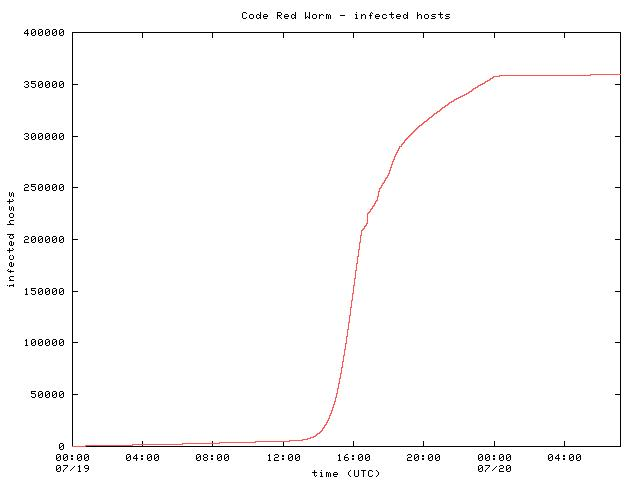
\includegraphics[scale=.6]{cumulative-ts.jpg}
	\caption{Multiplicarea viermelui Code Red versiunea a doua pe data de 19 iulie 2001}
	\label{multcodered}
\end{figure}

Curba din figura \ref{multcodered} are o form'a numit'a ``sigmoid'a'', av'jnd dou'a zone distincte: 
\begin{itemize}
	\item O zon'a 'in care infec'tia urmeaz'a o curb'a exponen'tial'a; 'inceputul este lent, rata de infec'tie fiind sc'azut'a, dar dup'a ce un numar suficient de mare de calculatoare este infectat, viteza cu care infectia se rasp'indeste este uluitoare;
	\item O zon'a 'in care infec'tia se plafoneaz'a la o valoare limit'a; 'in cazul acestui vierme, aceast'a limit'a a fost atins'a pentru c'a viermele era pre-programat s'a-'si opreasc'a multiplicarea la ora 24;
\end{itemize}

Chiar dac'a viermele nu este pre-programat sa se opreasc'a, trebuie s'a ne a'stept'am ca viteza de infectie s'a urmareasc'a o astfel de curb'a. De fapt, similitudinea cu un organism biologic este din nou frapant'a: zoologii care studiaz'a evolu'tia unei popula'tii animale au descoperit aceast'a lege de 'inmul'tire cu mult timp 'in urm'a, 'si i-au dat 'si un nume, ``legea logistic'a''. 

Legea logistic'a poate fi descris'a printr-o formul'a aparent complicat'a, dar care, la o analiz'a atent'a, este foarte natural'a: 

\[
	\frac{dN}{dt} = rN\biggl(\frac{K - N}{K}\biggr),
\]

unde:

\begin{itemize}
	\item N - num'arul de noduri infectate, o func'tie de timp t; 
	\item r - ``rata infec'tiei'': num'arul de calculatoare pe care un nod infectat le infecteaz'a la r'jndul lui 'intr-o unitate de timp;
	\item K - o valoare numita de zoologi ``capacitatea mediului'': num'arul de indivizi care pot fi suporta'ti de resursele ecologice. 'In acest caz, K este popula'tia total'a de calculatoare care ruleaza programul defect. 
\end{itemize}

Se pot recunoa'ste 'in aceast'a lege cele dou'a p'ar'ti ale graficului:

\begin{enumerate}
	\item Zona ini'tiala, 'in care N este mic comparat cu K: 'in aceasta zon'a frac'tia \(\frac{K - N}{K}\) este aproximativ 1, 'si legea devine: \[\frac{dN}{dt} = rN,\] ceea ce prin integrare 'in raport cu timpul conduce la: \[N(t) \approx r^t,\] adic'a o curb'a exponential'a. Explicatia este evident'a: 'in prima generatie avem un calculator, 'in a doua el va infecta r calculatoare, 'in a treia fiecare va infecta alte r, deci vom avea \(r^2\), apoi \(r^3\), 's.a.m.d.
	
	\item C'jnd num'arul de calculatoare infectate N devine comparabil cu popula'tia K, tentativele de infec'tie nu vor mai fi la fel de eficace: mai multe calculatoare diferite vor infecta aceea'si victim'a, deci genera'tia va cre'ste mai pu'tin de r ori. La limit'a, c'jnd toate calculatoarele sunt infectate, adic'a \(K = N\), avem \(\frac{K - N}{K} = 0\), deci \[\frac{dN}{dt} = 0,\] ceea ce 'inseamn'a c'a popula'tia r'am'jne constant'a de-a lungul timpului. [Frac'tia \(\frac{K - N}{K}\) reprezit'a probabilitatea ca un calculator neinfectat s'a fie infectat, adic'a num'arul de calculatoare neinfectate supra num'arul total de calculatoare.] 
\end{enumerate}

Partea alarmant'a a acestei 'int'jmplari este c'a 'in doar 24 de ore infec'tia a acoperit aproape o jum'atate de milion de calculatoare! 
%3.6.4
%3.6

%CapIII Tipuri de atacuri pe internet

%CapIV Ziduri de foc
\chapter{Ziduri de foc}

%4.1
\section{Tipuri}
Unele persoane definesc un firewall ca fiind ``o cutie proiectat'a pentru a filtra traficul spre 'si dinspre Internet'', ceva ce po'ti construi sau cump'ara. Dar cine are un router se prea poate s'a aib'a deja un firewall. Majoritatea routere-lor 'incorporeaz'a filtre de pachete; depinz'jnd de tipul de securitate, acest filtru ar putea fi de ajuns. 'In alte situa'tii, un router poate face parte dintr-un sistem mai amplu, numit sistem firewall. A'sadar, nu este nevoie ca un firewall s'a fie o simpl'a cutie.

Un firewall este orice dispozitiv, aplica'tie sau echipament care limiteaz'a accesul la re'tea. Poate fi o cutie cump'arat'a sau construit'a, sau o aplica'tie care ruleaz'a la un anumit nivel 'in modelul OSI. Ast'azi firewall-urile vin ``gratis'' 'incorporate 'in mai multe tipuri de dispozitive: router-e, modem-uri, sta'tii wireless, switch-uri IP, etc. Aplica'tiile firewall sunt disponibile(sau chiar incluse 'in) majoritatea sistemelor de operare de pe pia't'a. Pot fi un ``adaos la calcularotul client'' 'intr-un PC care ruleaz'a Windows, sau un set de reguli de filtrare implementate 'in kernel-ul de Unix(IP tables). Calitatea acestor firewall-uri poate fi destul de bun'a: tehnologia a progresat destul de mult de la apari'tia Internetului.

Firewall-urile pot filtra la diferite nivele 'intr-o stiv'a de re'tea. Exist'a trei mari categorii: \emph{filtre de pachete}, \emph{``por'ti'' la nivel de circuit} 'si \emph{``por'ti'' la nivel de aplica'tie}. Ficare dintre acestea este caracterizat de nivelul din protocol pe care 'il controleaz'a, de la cel mai de jos, p'jn'a la cel mai de sus, dar aceste categorii ajung s'a se 'intrep'atrund'a p'jn'a la urm'a. De exemplu, un filtru de pachete, ruleaz'a la nivelul IP, dar poate s'a mai 'tin'a cont 'si de informa'tia din interiorul pachetului(informa'tie TCP de exemplu), care se situeaz'a la nivelul \emph{circuit}. 'In general, mai multe tipuri diferite sunt folosite 'in acela'si timp. Exist'a, de asemeneam un al patrulea tip: \emph{filtru de pachete dinamic}. Acesta este o combina'tie dintre un filtru de pachete 'si un filtru la nivel de circuit(deseori 'incorporeaz'a 'si filtrare la nivel de aplica'tie).

\begin{figure}[ht]
	\centering
	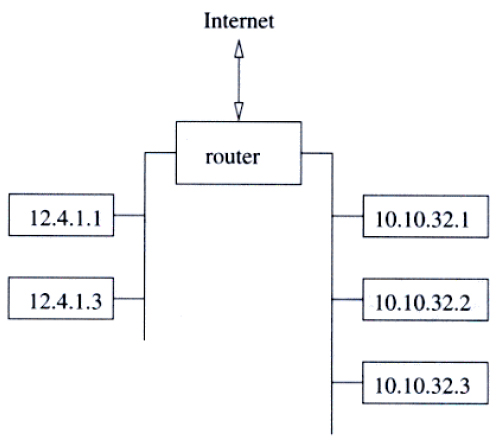
\includegraphics[scale=.6]{firerouter.jpg}
	\caption{O simpl'a mic'a re'tea de cas'a sau de companie. Gazdele din dreapta au adrese private, 'si nu pot fi contactate din arara router-ului. Gazdele din st'jnga sunt gazde normale. Ele pot vorbi unele cu altele. Pentru a ataca o gazd'a din dreapta, una din gazdele din st'jnga trebuie compromos'a. 'Intr-un anumit sens, router-ul se comport'a ca un firewall, chiar dac'a singurele reguli de filtrare pot fi o parte din informa'tiile de rutare.}
	\label{firerouter}
\end{figure}

Exist'a si alte metode care pot limita accesul la re'tea din afar'a. S'a consider'am re'teaua din figura \ref{firerouter}. Aceast'a re'tea are dou'a ramuri: una con'tine gazde rezistente la atac, cealalt'a are sisteme fie foarte susceptibile la un atac sau far'a nevoie de acces la Internet(de exemplu, imprimante). Gazdele din prima subre'tea au acces rutabil la Internet, iar cele din cea de-a doua au adresare de tip RFC 1918(adrese private). Cele dou'a subre'tele pot comunica 'intre ele, dar gazde din afara re'telei pot comunica doar cu gazdele din prima subre'tea. Nici un mod de a ajunge la cea de-a doua subre'tea nu exist'a 'in afar'a de ``a rico'sa pachete'' prin gazdele accesibile sau a compromite una dintre aceasta('In unele medii este posibil s'a se ating'a acela'si efect chiar f'ar'a folosirea unui router, prin simpla 'impar'tire a aceluia'si fir de cele dou'a subre'tele).
%4.1

%4.2
\section{Filtre de pachete}
Filtrele de pachete pot asigura un mijloc destul de ieftin 'si util de securitate. De obicei abilit'a'tile de filtrare vin cu soft-ul router-ului, pentru c'a probabil este nevoie de un router pentru conectarea la Internet oricum. A'sadar, nu va costa nimic 'in plus.

Filtrele de pachete func'tioneaz'a prin blocarea pachetelor bazat'a pe adresa surs'a 'si adresa destina'tie sau numerele de port. 'In cele mai multe cazuri nu se 'tine cont de context; deciziile sunt luate pe baza con'tinutului pachetului curent. Depinz'jnd de tipul de router, filtrarea poate fi f'acut'a la interfa'ta ``dinspre'' Internet, la interfa'ta ``spre'' Internet, sau la ambele. Adminstratorul alc'atuie'ste o list'a cu adresele 'si serviciile acceptate 'si o list'a cu adresele 'si serviciile neacceptate. Este destul de simplu s'a se permit'a sau nu accesul la nivelul unei gazde sau unei re'tele cu un filtru de pachete. De exemplu, se poate permite orice tip de acces 'intre gazdele A 'si B, sau se poate bloca orice tip de acces la B de la orice alt sistem 'in afar'a de A.

Filtrele de pachete sunt bune pentru a bloca pachete de tip spoof, fie care vin spre re'tea sau care pleac'a de la re'tea. Un ISP se poate asigura c'a orice client va emite doar pachete cu adrese surs'a valide(acest tip de filtrare se nume'ste \emph{ingress filtering}). Prin intermediul acestor mecanisme se poate, de asemenea, asigura c'a pachetele care vin spre re'tea nu au adresa surs'a o adres'a care apar'tine re'telei. Se poate aplica 'si tehnica \emph{egress filtering}: asigurarea c'a o gazd'a din re'tea nu emite pachete cu adrese necorespunz'atoare.

Majoritatea politicilor de securitate cer un control mai bun dec'jt cel oferit de filtrele de pachete. De exemplu, un adinistrator ar putea s'a doreasc'a s'a permit'a oric'arei gazde s'a se conecteze la gazda A, dar doar pentru a trimite sau a primi e-mail. Alte servicii ar putea sau nu s'a fie permise. Filtrele de pachete au acces 'si pot controla c'jt de c'jt acest nivel, dar este un proces periculos 'si expus erorilor. Pentru a putea folosi un filtru de pachete 'in acest fel, este nevoie de o bun'a cunoa'stere a utiliz'arii porturilor TCP 'si UDP pe diferite sisteme de operare.

Acesta este unul din motivele pentru care filtrele de pachete nu reprezint'a o solu'tie fiabil'a 'intotdeauna. Sunt destul de bune atunci c'jnd politica de securitate este simpl'a, dar c'jnd trebuie implementate reguli mai complicate, o simpl'a gre'seal'a poate 'inr'aut'a'ti lucrurile destul de mult din perspectiva securit'a'tii, l'as'jnd o gaura de exploatat pentru un eventual atacator. Chiar 'si cu un filtru perfect implementat, unele compromisuri pot fi periculoase.

Configurarea unui filtru de pachete este un proces 'in trei pa'si. Mai 'int'ji trebuie 'stiut ce va fi permis 'si ce nu(adic'a o politic'a de securitate). 'In al doilea r'jnd tipurile de pachete permise trebuie specificate formal, prin expresii logice pe c'jmpurile dintr-un pachet. Ultimul pas(care poate fi destul de dificil) const'a 'in scrierea expresiilor 'in sintaxa suportat'a de firewall.

Iat'a un exemplu. S'a presupunem c'a politca de securitate permite primirea e-mail(SMTP, port 25), dar doar sistemului gateway. 'In plus, e-mail-ul care vine de la un anumit site(SPIGOT) este blocat, fiind considerat spam. Un filtru care ar implementa un astfel de set de reguli poate ar'ata 'in felul urm'ator:

\begin{table}[ht]
	\centering
	\begin{tabular}{c|c|c|c|c|c}
		ac'tiune & gazd'a local'a & port & gazd'a la distan't'a & port & comentariu\\
		\hline
		blocheaz'a & * & * & SPIGOT & * & nu avem 'incredere 'in acest site\\
		permite & OUR-GW & 25 & * & *	&
	\end{tabular}
	\label{tab:rul1}
\end{table}

Aceste reguli sunt aplicate 'in ordine de sus 'in jos. Pachetele care nu sunt 'in mod explicit permise de o regul'a sunt respinse. Cu alte cuvinte, orice set de reguli are la sf'jr'sit o regul'a implicit'a:

\begin{table}[ht]
	\centering
	\begin{tabular}{c|c|c|c|c|c}
		ac'tiune & gazd'a local'a & port & gazd'a la distan't'a & port & comentariu\\
		\hline
		blocheaz'a & * & * & * & * & implicit\\
	\end{tabular}
	\label{tab:rul2}
\end{table}

Aceast'a metod'a se pliaz'a pe filosofia: tot ceea ce nu este 'in mod explicit permis, este blocat.

Se observ'a diferen'ta dintre primul set de reguli 'si ur'atoarea, care 'inseamn'a ``orice gazd'a intern'a poate trimite mail c'atre exterior'':

\begin{table}[ht]
	\centering
	\begin{tabular}{c|c|c|c|c|c}
		ac'tiune & gazd'a local'a & port & gazd'a la distan't'a & port & comentariu\\
		\hline
		permite & * & * & * & 25 & permite conexiunile SMTP spre exterior \\
	\end{tabular}
	\label{tab:rul3}
\end{table}

Cererea de conexiune poate veni de la orice port al unei gazde din re'tea spre portul 25 al unei gazde exterioare. Acest set de reguli pare simplu 'si evident. Este, de asemenea, gre'sit. Problema const'a 'in faptul c'a restric'tia definit'a este bazat'a numai pe num'arul de port al gazdei exterioare. 'In timp ce portul 25 este, 'intr-adev'ar, portul pentru e-mail, nu exist'a nici o modalitate de a controla acest lucru la o gazd'a str'ain'a. Un inamic poate accesa orice ma'sin'a din interiorul re'telei pe orice port dac'a cererea de conexiune pleac'a de la portul 25 al gazdei exterioare.

O regul'a mai bun'a ar fi s'a se permit'a doar cererile care pleac'a spre portul 25(outgoing). Adic'a gazdele trebuie l'asate s'a fac'a cereri spre portul 25 al unei ma'sini exterioare. Din fericire, distinc'tia dintre cererile spre re'tea(incoming) 'si cererile care pleac'a(outgoing) poate fi f'acut'a 'intru filtru de pachete simplu, dac'a expand'am no'tiunea.

O conexiune TCP consist'a din pachete care merg 'in ambele direc'tii. Chiar dac'a toate datele merg 'intr-un singur sens, pachete de confirmare 'si control vor circula 'si 'in sensul opus. Se poate duce la bun sf'jr'sit acest lucru prin examinarea direc'tiei unui pachet 'si prin examinarea unor c'jmpuri de control. 'In TCP pachetul ini'tial de cerere nu are bitul ACK setat 'in antet, restul pachetelor 'il au(de fapt, exist'a unele excep'tii rare 'in care va fi setat doar bitul RST). A'sadar, pachetele cu bitul ACK setat fac parte dintr-o conexiune stabilit'a; pachetele f'ar'a acest bit setat reprezint'a mesaje pentru stabiliri de conexiuni. Secretul const'a 'in permiterea pachetelor f'ar'a bitul ACK care pleac'a doar de la gazde interne(adic'a cereri de conexiune spre exterior). Ideea de baz'a este c'a o ma'sin'a exterioar'a nu poate ini'tia o conexiune, dar poate continua una.
Iat'a cum ar putea ar'ata implementarea acestei reguli 'in tabelul \ref{tab:rul4}.

\begin{table}[ht]
	\centering
	\begin{tabular}{c|c|c|c|c|c|c}
		ac'tiune & surs'a & port & destina'tie & port & c'jmpuri & comentariu\\
		\hline
		permite & {gazde locale} & * & * & 25 &  & locale spre 25 \\
		permite & * & 25 & * & * & ACK & raspuns exterior \\
	\end{tabular}
	\caption{Reguli de filtrare}
	\label{tab:rul4}
\end{table}

Nota'tia ``{gazde locale}'' descrie un set de ma'sini, oricare dintre acestea fiind eligibil'a. 'Intr-un filtru de pachete real se poate specifica explicit fiecare gazd'a sau se poate specifica un grup de ma'sini, probabil prins specificarea adresei de re'tea(de exemplu: 10.2.42.0/24).

%4.2.1
\subsection{Topologia re'telei 'si adrese spoof-ate}
Din motive economice, se poate dori folosirea unui singur router 'si ca un firewall 'si pentru a ruta trafic interior-interior. Un exemplu este constituit de figura \ref{rutxnet}. Exist'a patru re'tele, una extern'a 'si trei interne. Net 1 este o arie DMZ(demilitarized zone, care 'in contextul firewall-urilor se refer'a la o parte din re'tea care nu face parte nici din re'teaua intern'a, nici din Internet) compus'a doar dintr-o ma'sin'a de tip ``poart'a''(gateway). 

\begin{figure}[ht]
	\centering
	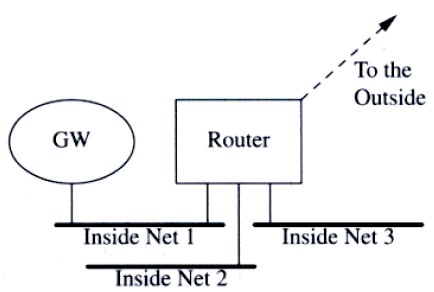
\includegraphics[scale=.6]{rutxnet.jpg}
	\caption{Un router de tip firewall cu multiple re'tele locale.}
	\label{rutxnet}
\end{figure}

Politicile de securitate sunt urm'atoarele:

\begin{itemize}
	\item conexiuni foarte limitate sunt permise 'intre ``poart'a'' 'si lumea exterioar'a; 
	\item conexiuni destul de limitate, dar posibil diferite, sunt permise 'intre gateway 'si orice sistem din Net2 sau Net3(protec'tie 'in caz c'a gateway-ul este compromis);
	\item cereri spre exterior sunt permise doar pentru Net2 'si Net3;
	\item orice este permis 'intre Net2 'si Net3.
\end{itemize}

Aceast'a situa'tie este foarte dificil'a. Mai 'int'ji , o regula care permite accesul deschis la Net2 trebuie s'a se bazeze pe o adres'a surs'a care apar'tine Net3. Apoi, nimic nu 'impiedic'a un atacator s'a trimit'a pachete din exterior care au ca adres'a surs'a, o adres'a din interior. Informa'tia vital'a conform c'areia pachete de la Net3 legitime pot sosi doar pe un anumit ``fir'', este neglijat'a.

Atacurile ip-spoofing ca acestea sunt dificil de implementat, dar nu sunt imposibile. De exemplu atacurile care folosesc ``ip source routing'' constituie o solu'tie pentru un eventual atacator, daca firewall-ul nu filtreaz'a aceste tipuri de pachete. Exist'a 'ins'a 'si atacuri mai complexe. Detectarea lor este practic imposibil'a f'ar'a folosirea filr'arii pe baza de adres'a 'si fi'sierelor log.

Acete m'asuri nu elimin'a 'ins'a toate atacurile posibile prin address-spoofing. Un atacator poate impresona o gazd'a care este de 'incredere 'si nu se afl'a 'in re'teaua intern'a. Ca urmare nu se recomand'a a avea 'incredere 'in gazde din afara controlului administrativ.

S'a presupunem c'a filtrarea se face pe input(interfa'ta spre Internet a firewall-ului, pachetele care vin), 'si c'a se dore'ste s'a se permit'a orice cerere spre exterior, dar cererile dinspre exterior sunt permise doar pentru mail, 'si numai c'atre gateway. Regulile ar trebui s'a arate asem'an'ator cu cele din tabelul \ref{tab:rul5}.

\begin{table}[ht]
	\centering
	\begin{tabular}{c|c|c|c|c|c|c}
		ac'tiune & surs'a & port & destina'tie & port & c'jmpuri & comentariu\\
		\hline
		blocheaz'a & {Net 1} & * & * & * &  & blochez'a spoof \\
		blocheaz'a & {Net 2} & * & * & * &  & blochez'a spoof \\
		blocheaz'a & {Net 3} & * & * & * &  & blochez'a spoof \\
		permite & * & * & GW & 25 &  & cereri legale \\
		permite & * & * & {Net 2} & * & ACK & r'aspunsuri \\
		permite & * & * & {Net 3} & * & ACK & r'aspunsuri \\
	\end{tabular}
	\caption{Reguli de filtrare}
	\label{tab:rul5}
\end{table}

Aceste reguli presupun blocarea adreselor false(pachete cu adrese surs'a care apar'tin re'telei nu pot sosi dinspre exterior), permiterea pachetelor dinspre exterior dac'a sunt pentru serverul de mail, sau dac'a fac parte dintr-o conversa'tie stabilit'a deja prinr-o cerere a ma'sinilor locale. Orice altceva va fi blocat.

Setul de reguli pe interfa'ta spre Net1 ar trebui s'a fie pu'tin mai nerestrictiv'a. Ar trebui s'a se blocheze cererile interne nerestric'tionate, chiar 'si de la gateway. S-ar putea opta doar pentru permiterea livr'arii mail-ului. 'In cazul de fa'ta gateway-ul va vorbi direct doar cu alte ma'sini care ruleaz'a servere de mail de 'incredere(eventual diferite de cel rulat de gateway, pentru c'a dac'a un atacator descoper'a un mod de a compromite aplica'tia de mail de pe gateway, probabil va putea compromite 'in acela'si mod 'si gazdele interne care ruleaz'a aceea'si aplica'tie). O astfel de ma'sin'a se nume'ste \emph{gateway intern}. Iat'a o posibil'a configurare a regulilor pe interfa'ta spre Net1 'in tabelul \ref{tab:rul6}.

\begin{table}[ht]
	\centering
	\begin{tabular}{c|c|c|c|c|c|c}
		ac'tiune & surs'a & port & destina'tie & port & c'jmpuri & comentariu\\
		\hline
		permite & GW & * & {parteneri} & 25 &  & conexiuni SMTP \\
		permite & GW & * & {Net 2} & * & ACK & r'aspunsuri cereri interne \\
		permite & GW & * & {Net 3} & * & ACK &  \\
		blocheaz'a & GW & * & {Net 2} & * &  & blochez'a alt tip acces GW \\
		blocheaz'a & GW & * & {Net 3} & * &  &  \\
		permite & GW & * & * & * &  & permite acces GW spre exterior  \\
	\end{tabular}
	\caption{Reguli de filtrare}
	\label{tab:rul6}
\end{table}

Din nou, este prevenit spoofing-ul, deoarece toate regulile spceific'a gateway-ul; doar aceast'a ma'sin'a ar trebui s'a existe 'in aceast'a subre'tea, as'a c'a nimic altceva nu trebuie permis.

Dac'a sunt folosite router-e care suport'a doar filtrare spre exterior, topologia recomandat'a este asem'anatoare figurii \ref{fireinout}. Acum este nevoie de dou'a router-e s'a 'indeplineasc'a sarcina pe care mai devreme un singur router o putea 'indeplini(Figura \ref{2outfire}). 'In punctul (a) se folose'ste setul de reguli care protejeaz'a re'teaua interioar'a de un gateway compromis 'si 'in punctul (b) se folose'ste setul de reguli care protejeaz'a 'impotriva falsific'arii adreselor IP(spoofing) 'si restric'tioneaz'a accesul doar la ma'sina gateway. Regulile nu trebuie schimbate absolut deloc. O regul'a de filtrare pus'a la intrare pe un port este echivalent'a cu o regul'a pus'a la ie'sire pe cel'alalt port.

\begin{figure}[ht]
	\centering
	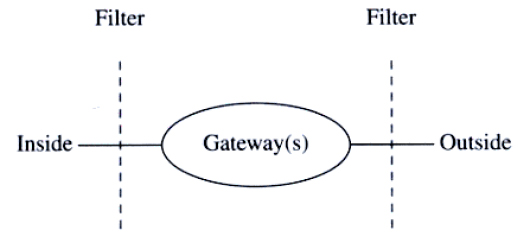
\includegraphics[scale=.6]{fireinout.jpg}
	\caption{Schema unui firewall.}
	\label{fireinout}
\end{figure}

\begin{figure}[ht]
	\centering
	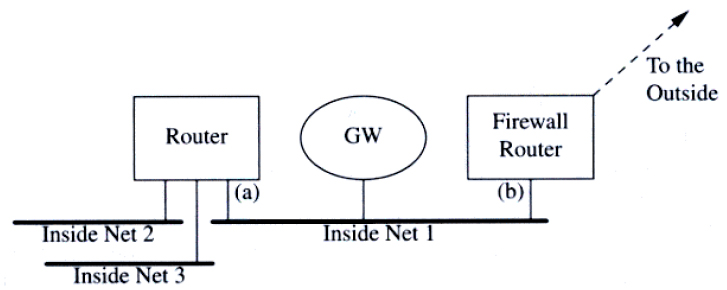
\includegraphics[scale=.6]{2outfire.jpg}
	\caption{Un firewall cu filtre spre exterior.}
	\label{2outfire}
\end{figure}

Filtrele de intrare permit router-ului s'a nu primeasc'a pachetele care 'il au ca 'tint'a pe el(de exemplu 'in cazul unui atac DDoS asupra unui router).
S'a consider'am regula din tabelul \ref{tab:rul7}.

\begin{table}[ht]
	\centering
	\begin{tabular}{c|c|c|c|c|c|c}
		ac'tiune & gazd'a local'a & port & gazd'a la distan't'a & port & c'jmpuri & comentariu\\
		\hline
		permite & * & * & ROUTER & * &  & prevenire acces router \\
	\end{tabular}
	\caption{Blocarea pachetelor destinate router-ului}
	\label{tab:rul7}
\end{table}

Aceast'a regul'a blocheaz'a toate pachetele destinate 'insu'si firewall-ului. Este probabil prea strict'a. Aproape 'intotdeauna este nevoie s'a se permit'a mesajele de rutare, sau r'aspunsurile pentru anumite mesaje de diagnosticare ce pot fi trimise de router. Regula general'a este 'ins'a: \emph{dac'a nu este nevoie de un serviciu, acesta trebuie eliminat!}.

'Inc'a un lucru mai trebuie punctat 'in aceast'a situa'tie(folosirea unui router care nu are filtru pentru input). Leg'atura extern'a 'catre un router firewall este, de obicei, o simpl'a linie serial'a c'atre router-ul ISP-ului. Dac'a se vrea a se avea 'incredere 'in provider, filtrarea se poate face pe partea de output a acelui router, ceea ce permite folosirea topologiei expuse 'in figura \ref{rutxnet}. Totu'si m'asuri de precau'tie sunt necesare deoarece router-ul provider-ului probabil serve'ste mai mul'ti clien'ti 'si, ca urmare, poate fi subiectul deselor schimb'ari de configura'tie.
%4.2.1

%4.2.2
\subsection{Filtre de rutare}
Filtrarea informa'tiei de rutare este foarte important'a. De aceea router-ele trebuie s'a fie capabile s'a controleze informa'tiile de rutare 'inaintate pe diferite interfe'te.

S'a consider'am figura \ref{rutxnet}. De aceast'a dat'a vom presupune c'a gazdelor din Net2 'si Net3 nu le este permis accesul direct spre exterior. Sunt conectate la router a'sa c'a pot vorbi cu 'intre ele 'si cu gazda gateway din Net1. 'In acest caz router-ul nu ar trebui s'a 'inainteze spre alte router-e c'aile c'atre Net2 'si Net3. Mecanismele de configurare a router-ului trebuie s'a fie suficient de sofisticate pentru a permite acest lucru. Solu'tia const'a 'in 'inaintarea informa'tiei doar despre Net1 'si blocarea oric'arui tip de informa'tie care con'tine c'ai spre gazdele din Net1 'si Net2. Cea mai bun'a alegere este folosirea adreselor private(RFC 1918). 

Exist'a totu'si o situa'tie 'in care se poate contacta o astfel de gazd'a: dac'a este permis'a ``IP source routing''. Majoritatea router-elor pot s'a blocheze astfel de pachete; dac'a un router are aceast'a op'tiune, este bine s'a fie folosit'a deoarece un atacator poate folosi aceast'a tehnic'a nu numai pentru a ajunge la o gazd'a ``de neatins'', dar 'si pentru atacuri address-spoofing. Exist'a destule probleme ce 'tin de implementare 'in ceea ce prive'ste aceast'a optiune oferit'a de IP(source routing): unele routere au buguri 'in procesul de blocare a acestui tip de pachete; chiar 'si gazdele pot avea buguri 'in tratarea acestor pachete(un atacator poate la fel de bine s'a blocheze sistemul unei gazde sau s'a 'il penetreze).

Dac'a se blocheaz'a pachetele cu source-routing, 'si, in general, nu exist'a nici un motiv pentru a nu face acest lucru, acestea trebuie blocate mai degrab'a la router-ele de grani't'a dec'jt la cele din backbone. Pe l'jng'a cerin'tele de vitez'a pentru router-ele din backbone, dac'a este vorba de o re'tea cu o topologie complex'a(un ISP sau o companie mare), unele opera'tii din interiorul re'telei pot avea nevoie de folosirea source-routing pentru testarea comenzilor \emph{ping} 'si \emph{traceroute}.

Filtrele trebuie de asemenea aplicate rutelor primite de un router din afar'a. Acest lucru este necesar pentru evitarea compromiterii prin folosirea de informa'tie de rutare eronat'a. De exemplu, s'a presupunem c'a un atacator 'stie c'a gazda A din subre'teaua 1 are 'incredere 'in gazda Z din subre'teaua 100. Dac'a o ruta fals'a este c'atre subre'teaua 100 care are o cale mai scurt'a dec'jt cea legitim'a este injectat'a 'in re'tea, gazda A poate fi p'ac'alit'a s'a cread'a c'a ruta spre gazda Z trece prin ma'sina atacatorului. Acesta permite impersonarea adev'aratei gazde Z de c'atre atacator.

'Intr-o oarecare m'asur'a, filtrele de pachete elimin'a nevoia pentru filtrele de rute. Dac'a cererile rlogin nu sunt permise printr-un firewall, nu conteaz'a dac'a ruta c'atre gazda Z este fals'a; cererea rlogin va fi blocat'a oricum. Dar injectarea de rute false 'inc'a poate fi folosit'a pentru a corupe comunicarea legitim'a dintre gateway 'si gazdele interne.

Ca 'si 'in cazul filtr'arii pe baz'a de adres'a, filtrarea rutelor devine dificil'a 'si chiar imposibil'a 'in cazul topologiilor complexe.
%4.2.2

%4.2.3
\subsection{Configura'tii posibile}
Desigur, configura'tia unui filtru de pachete depinde de politica de securitate, dar exist'a c'jteva exemple rezonabile care pot constitui un punct de plecare. Exemplele din tabelele \ref{tab:rul8} 'si \ref{tab:rul9} fac parte din recomandarea CERT.

\begin{table}[ht]
	\centering
	\begin{tabular}{c|c|c|c|c|c|c}
		ac'tiune & gazd'a local'a & port & gazd'a la distan't'a & port & op'tiuni & comentariu\\
		\hline
		permite & SECONDARY & * & OUR-DNS & 53 &  & DNS scundar \\
		blocheaz'a & * & * & * & 53 &  & bl. rest DNS \\
		permite & * & * & * & 53 & UDP & DNS peste UDP \\
		permite & NTP.OUTSIDE & 123 & NTP.INSIDE & 123 & UDP & acces NTP \\
		blocheaz'a & * & * & * & 69 & UDP & bl. TFTP \\
		blocheaz'a & * & * & * & 87 &  &  \\
		blocheaz'a & * & * & * & 111 &  & bl. TCP RPC \\
		blocheaz'a & * & * & * & 111 & UDP & bl. UDP RPC \\
		blocheaz'a & * & * & * & 2049 & UDP & bl. NFS \\
		blocheaz'a & * & * & * & 2049 &  & bl. NFS \\
		blocheaz'a & * & * & * & 512 & UDP & bl. ``r'' \\
		blocheaz'a & * & * & * & 513 &  & ... \\
		blocheaz'a & * & * & * & 514 &  & ... \\
		blocheaz'a & * & * & * & 515 &  &  \\
		blocheaz'a & * & * & * & 540 &  &  \\
		blocheaz'a & * & * & * & 6000-6100 &  &  \\
		permite & * & * & ADMINNET & 443 &  &  \\
		blocheaz'a & * & * & ADMINNET & * &  &  \\
		blocheaz'a & PCLAB-NET & * & * & * &  &  \\
		blocheaz'a & PCLAB-NET & * & * & * & UDP &  \\
		permite & * & * & * & * &  & TCP - Ok \\
		blocheaz'a & * & * & * & * & UDP & UDP - not Ok \\
	\end{tabular}
	\caption{Reguli de filtrare pentru o universitate. Regulile care nu se refer'a explicit la UDP sunt pentru TCP.}
	\label{tab:rul8}
\end{table}

\begin{table}[ht]
	\centering
	\begin{tabular}{c|c|c|c|c|c|c}
		ac'tiune & gazd'a local'a & port & gazd'a la distan't'a & port & op'tiuni & comentariu\\
		\hline
		permite & * & * & MAIGATE & 25 &  & acces la mail \\
		permite & * & * & MAIGATE & 53 & UDP & acces la DNS \\
		permite & SECONDARY & * & MAIGATE & 53 &  & DNS secundar \\
		permite & * & * & MAIGATE & 23 &  & acces telnet \\
		permite & NTP.OUTSIDE & 123 & NTP.INSIDE & 123 & UDP & acces NTP \\
		permite & INSIDE-NET & * & * & * &  & pachete exterior Ok \\
		permite & * & * & INSIDE-NET & * & ACK & permite r'aspunsurile \\
		blocheaz'a & * & * & * & * &  & blocheaz'a restul \\
		blocheaz'a & * & * & * & * & UDP & blocheaz'a restul \\
	\end{tabular}
	\caption{Reguli de filtrare pentru o companie mic'a.}
	\label{tab:rul9}
\end{table}

O universitate tinde s'a aib'a o politic'a deschis'a 'in ceea ce prive'ste conexiunile la Internet. Totu'si trebuie s'a blocheze unele servicii, cum ar fi NFS 'si TFTP. Nu are nici un sens s'a asigure astfel de servicii. De asemenea, poate c'a a existat un laborator care a fost cauza unor probleme, ca urmare, accesul la Internet va fi blocat pentru acesta. Nu va exista acces la nodurile administrative cu excep'tia unui singur serviciu(transcript manager) care func'tioneaz'a peste HTTPS(HTTP secure) 'si care foloses'te mijloace puternice de autentificare 'si criptografie.

O companie mic'a sau chiar o re'tea de ``cas'a'' cu o conexiune la Internet poate dori s'a blocheze o parte din traficul spre re'tea, 'in timp ce permite marea parte din traficul spre exterior. Un gateway prime'ste mail 'si asigur'a servicii de nume pentru restul gazdelor. Dac'a serverele de DNS 'si mail ale companiei sunt rulate de ISP, aceste reguli pot fi simplificate 'si mai mult. 

'In orice caz, filtrele de pachete sunt considerate inadecvate 'in cazul c'jnd filtrarea se face la nivel de port. 'In cazul universita'tii 'in special, aceste filtre pot 'incetini atacatori experimenta'ti, dar probabil nu 'ii pot opri.
%4.2.3

%4.2.4
\subsection{Performan'ta filtrelor de pachete}
Exist'a un pre't ce trebuie pl'atit pentru filtrele de pachete: o mic'a sc'adere a performan'tei ruter-elor. Acestea sunt 'in general optimizate pentru a ruta pachetele c'jt se poate de repede. Filtrele de pachete r'apesc din timpul de procesare 'si pot anula eforturile de optimizare, dar acestea sunt de obicei pozi'tionate la marginea unui domeniu administrativ. Pentru aceste router-e bottleneck-ul este reprezentat de cele mai multe ori de leg'atura serial'a, ceea ce 'inseamn'a c'a CPU-ul are detul timp s'a parcurg'a c'jteva tabele de reguli.

Sc'aderea performan'tei depinde de num'arul de reguli impuse. 'In general, este mai bine s'a fie o singur'a regul'a care s'a specifice o subre'tea dec'jt mai multe reguli care s'a enumere fiecare gazd'a din subre'tea. Alegerea aceastei optimiz'ari 'inseamn'a ca gazdele vor accepta acelea'si restric'tii; dac'a acest lucru este posibil sau nu, depinde de configurarea re'telei. Exist'a posibilitatea mic'sor'arii timpului de procesare prin ordonarea regulilor astfel 'inc'jt cele mai comune tipuri de trafic sunt procesate promele(desigur, trebuie mult'a aten'tie pentru aceast'a ac'tiune, deoarece securitatea este mai important'a dec'jt viteza).
%4.2.4
%4.2

%4.3
\section{Filtrarea la nivel de aplica'tie}
Un filtru de pachete nu are nevoie s'a 'inteleag'a traficul pe care 'il limiteaz'a. Verific'a adresele surs'a 'si destina'tie 'si se poate uita 'in antetul UDP sau TCP la porturi sau campurile pentru op'tiuni.

Filtrele la nivel de aplica'tie se confrunt'a cu detalii ale serviciilor pe care le verific'a 'si de obicei sunt mai complexe dec'jt filtrele de pachete. Filtrele la nivel de aplica'tie nu folosesc un mecanism cu scop general pentru filtrarea mai multor tipuri de trafic. 'In schimb, cod specializat pentru fiecare tip de serviciu poate fi folosit pentru fiecare aplica'tie dorit'a. De exemplu, un filtru la nivel de aplica'tie pentru e-mail va 'in'telege antetele specificate 'in RFC 822, formatul MIME 'si ar putea fi chiar capabil s'a identifice sofware infec'tios.

Gateway-urile la nivel de aplica'tie au un alt avantaj care 'in unele cazuri poate fi critic: usurin'ta de a loga 'si de a controla tot traficul, 'in ambele sensuri. Mail-urile pot fi verificate pentru prezent'a cuvintelor obscene, sau se poate verifica dac'a date confiden'tiale trec prin acest gateway. Cererile web pot fi verificate pentru conforman't'a cu politicile companiei, 'si ata'samentele periculoase ale mail-urilor pot fi 'indep'artate.

Mesaje ale po'stei electronice sunt trecute de obicei printr-un gateway la nivel de aplica'tie, indiferent de ce tehnologie este folosit'a la restul firewall-ului. Chiar 'si f'ar'a firewall gateway-urile de mail pot fi pre'tioase pentru celelalte calit'a'ti. Numele ma'sinilor interne poate fi mascat, ascunz'jnd astfel date valoroase. Analiz'a de trafic sau de con'tinut 'si 'inregistr'ari pot fi f'acute pentru a c'auta eventuale scurgeri de informa'tie.

Aceste mecanisme sunt f'acute pentru a proteja 'impotriva atacurilor din exterior. Un atacator din interiorul re'telei nu va putea fi oprit de ele. Dar acest scenariu nu reprezint'a problema firewall-urilor 'in general.

Principalul dezavantaj al gateway-urilor la nivel de aplica'tie este nevoia pentru un program cu interfa't'a utilizator specializat pentru fiecare serviciu ce trebuie monitorizat. 'In practic'a, acest lucru 'inseamn'a ca numai cele mai importante servicii vor fi suportate. O mare problem'a este reprezentat'a de protocoalele private: ceva ce nu se cunoa'ste nu poate fi filtrat. Unele firewall-uri comerciale includ o suit'a larg'a de astfel de gateway-uri la nivel de aplica'tie. Semn'jnd contracte cu majoritatea companiilor, pot ad'auga suport pentru numeroase protocoale private. Cu toate acestea 'inc'a r'am'jne o 'intrebare: se dore'ste rularea multor programe ``ciudate'' 'in plus - gateway-urile per-aplica'tie ale firewall-ului?
%4.3

%4.4
\section{Gateway-uri la nivel de circuit}
Gateway-urile la nivel de circuit func'tioneaz'a la nivelul TCP. Conexiunile TCP sunt trecute printr-un calculator care, se comport'a ca un ``cablu de tansisie'' din punctul de vedere al gazdei care ia parte la conexiune. Acest calculator ruleaz'a un program care copiaz'a octe'ti 'intre dou'a conexiuni, una cu gazda local'a 'si cealalt'a cu gazda exterioar'a. Gateway-ul poate loga anumite detalii sau salva con'tinutul conexiunii. 'In aceast'a schem'a, c'jnd un client vrea s'a se conecteze la un server, se conecteaz'a la gateway 'si 'ii ofer'a acestuia informa'tii despre tipul de conexiune printr-un protocol simplu. Gazda gateway se conecteaz'a apoi la serverul dorit. Numele 'si adresa IP a clientului nu este de obicei transmis'a serverului(serverul are impresia c'a ``discut'a'' doar cu gateway-ul).

Gateway-ul func'tioneaz'a deasupra nivelului IP, ceea ce 'inseamn'a ca anumite probleme, cum ar fi fragmentarea pachetelor sunt rezolvate la gateway. Interfa'ta spre Internet a gateway-ului transmite pachete normale TCP/IP.

Gateway-urile la nivel de circuit sunt, 'in general, folosite pentru a crea conexiuni specifice 'intre re'tele izolate. Din primele zile ale Internetului, multe companii 'i'si separau intraneturile de Internet la nivel de circuit. O astfel de configura'tie este expus'a 'in figura \ref{sockproxy}.

\begin{figure}[ht]
	\centering
	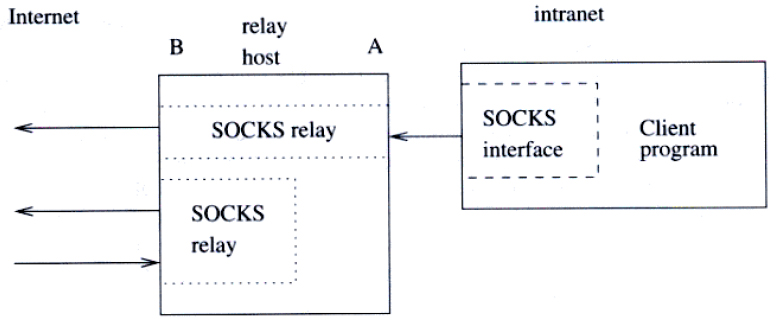
\includegraphics[scale=.5]{sockproxy.jpg}
	\caption{O conexiune obi'snuit'a SOCKS pe intrfa'ta A 'si o conexiune TCP/IP oarecare pe interfa'ta exterioar'a B. SOCKS este un protocol care permite aplica'tiilor client-server s'a foloseasc'a 'in mod transparent serviciile unui firewall.}
	\label{sockproxy}
\end{figure}

'In unele cazuri, o conexiune la nivel circuit e f'acut'a automat ca parte a arhitecturii gateway-ului. Un anumit serviciu TCP ar putea fi direc'tionat de la o gazd'a extern'a la un sistem de baze de date intern. Exist'a multe programe simple pentru a 'indeplini aceast'a func'tie, de exemplu ``tcprelay''.

'In alte cazuri, serviciul de conexiune trebuie s'a 'stie destina'tia dorit'a. 'In acest caz, exist'a un mic protocol 'intre gazd'a care cere conexiunea 'si gateway. Prin intermediul acestui protocol se poate descrie adresa 'si serviciul destina'tie(de asemenea, gateway-ul poate semnala erori dac'a este cazul). David 'si Michelle Koblas au implementat SOCKS, un astfel de protocol care este, 'in zilele noastre, unul din cele mai 'intrebuin'tate. Cei mai importan'ti clien'ti de pe Internet cunosc protocolul SOCKS 'si pot fi configura'ti s'a foloseasc'a gateway-uri SOCKS.

'In general, gateway-ul nu va examina octe'tii de informa'tie care circul'a 'in contextul unei conexiuni. Pot loga num'arul de octe'ti sau destina'tia TCP, ceea ce poate fi util 'in anumite cazuri. 

Orice circuit gateway(incluz'jnd SOCKS) implic'a faptul c'a gazda gateway ascut'a pe un port, pentru a implementa o conexiune FTP. Exist'a o problem'a subtil'a cu no'tiunea de gateway la nivel de circuit: utilizatorii necooperan'ti pot u'sor trece peste inten'tia celui care a proiectat gateway-ul, conect'jndu-se la servicii neautorizate. Este inprobabil, de exemplu, ca portul 25 s'a fie folosit 'in acest scop, din moment ce gateway-ul folose'ste acest port pentru propia conexiune SMTP, dar exist'a alte pericole. De exemplu: un serviciu telnet neprotejat pe un port non-standard, un server NFS, un joc multiplayer. Logarea poate ajuta la observarea unor abuzuri de acest gen, dar nu la toate. Un lucru 'in'telept este s'a se combine un gateway la nivel de circuit cu un filtru de pachete care s'a blocheze aceste tipuri de conexiuni.
%4.4

%4.5
\section{Filtre dinamice de pachete}
Filtrele dinamice de pachete sunt cea mai comuna tehnologie firewall. Inten'tia este de a permite orice aplica'tie client s'a func'tioneaze, 'in timp ce control total asupra traficului este oferit administratorilor.

'Intr-o oarecare m'asur'a, un filtru dinamic de pachete se comport'a ca un fitru obi'snuit de pachete. Pachetele transmise sunt examinate; dac'a satisfac criteriile impuse, le este permis'a trecerea. Dar pe l'jng'a acest lucru, sunt 'inregistrate pachetele spre exterior, 'si pachetele spre interior care apar'tin aceleia'si conexiuni sunt permise. Aceasta 'inseamn'a c'a se 'tine cont de semantica unei conexiuni(f'ar'a a se pune baza pe sintaxa antetului). Este astfel posibil'a monitorizarea conexiunilor UDP de'si nu are bitul ACK folosit de filtrele de pachete pentru a face acest lucru la TCP.

A'sa cum am men'tionat, filtrele obi'snuite de pachete au 'si alte limit'ari. Cel mai mare este reprezentat'a de canalul de date folosit de FTP. Este imposibil s'a se monitorizeze acest canal 'in mod transparent, f'ar'a ca aplica'tia s'a 'stie acest lucru. 'In cazul filtrelor dinamice, conexiunile pe portul 21 - canalul de comand'a pentru FTP - primesc un tratament special. Fluxul de comenzi este scanat 'si valorile pasate comenzii PORT sunt folosite pentru a updata tabela de reguli. Acela'si lucru poate fi f'acut cu comanda PASV, dac'a filtrul de pachet trebuie s'a restric'tioneze traficul spre exterior.

Strategii similare sunt folosite 'si pentru RPC. Examinarea con'tinutului pachetului permite controlul asupra invoc'arii anumitor servicii RPC. Cu alte cuvinte, am trecut de la \emph{filtrare pachetelor} la \emph{filtrarea conexiunilor}.

%4.5.1
\subsection{Op'tiuni de implementare}
Din punct de vedere conceptual, exist'a doua modalita'ti principale de a implementa un filtru dinamic de pachete. Calea evident'a este de a face schimb'ari 'in mod dinamic 'si automat 'in setul de reguli. Aceast'a modalitate nu este tocmai indicat'a deoarece seturile de reguli sunt destul de ``fragile'' iar ordonarea regulilor conteaz'a foarte mult. Nu este 'intotdeauna clar care schimb'ari sunt benigne 'si care nu sunt.

Exist'a un alt mod de implementare a acestor tipuri de firewall-uri, echivalent din punct de vedere al conceptelor de func'tionare, dar care ofer'a o mai mare securitate. 'In locul modific'arii tabelei de reguli, filtrul dinamic va folosi semantici asem'anatoare nivelului circuit descris mai devreme, prin ``terminarea'' conexiunii la chiar la firewall. Acesta va ini'tia cererea c'atre destina'tia propriu-zis'a. Datele vor fi apoi copiate 'intre cele dou'a conexiuni.

Pentru a observa cum func'tioneaz'a aceast'a schem'a trebuie s'a reamintim ca o conexiune TCP este caracterizat'a de cvadruplul $<$gazdasursa, portsursa, gazdadestinatie, portdestinatie$>$. Dar gazda destina'tie nu este neap'arat o alt'a ma'sin'a; mai degrab'a este orice proces care 'i'si asum'a aceast'a adres'a. Filtrul dinamic poate r'aspunde cu orice adres'a din punctul de vedere al celui care ini'tiaz'a conexiunea. C'jnd ini'tializeaz'a conexiunea spre destina'tia real'a, poate folosi adresa gazdei client ca 'si cum ar fi a lui(a se vedea figura \ref{dynamicfire}). Conexiunile sunt identificate nu doar pe baza celor partu parametri ci 'si pe interfa'ta la re'tea folosit'a.

\begin{figure}[ht]
	\centering
	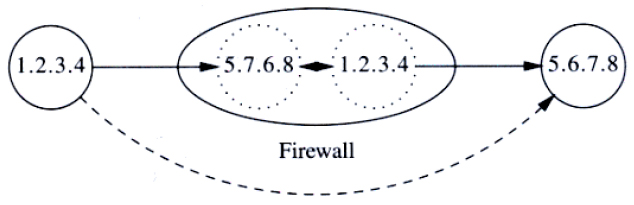
\includegraphics[scale=.6]{dynamicfire.jpg}
	\caption{Conexiunea printr-un filtru dinamic de pachete. S'ageata cu linie punctat'a indic'a conexiunea inten'tionat'a, iar s'age'tile cu linie continu'a indic'a conexiunile propriu-zise. Firewall-ul impresoneaz'a fiecare punct fa't'a de cel'alalt.}
	\label{dynamicfire}
\end{figure}

'In aceast'a situa'tie, pentru conexiunile TCP nu au nevoie de modific'ari substan'tiale(pu'tine modific'ari 'in cod), cu exept'ia copierii datelor(sau, mai degrab'a pointerilor c'atre adesele de memorie unde se afl'a datele) 'si a bi'tilor de op'tiuni. Aceea'si bucat'a de cod pentru a implementa mecanismul este folosit'a 'si la nivelul aplica'tie. Schimbarea adresei pachetului este, bine'in'teles, o opera'tie trivial'a. 

Semanticile de nivel aplica'tie, cum ar fi FTP proxy, se implementeaz'a foarte ``curat'' folosind aceast'a schem'a. 'In locul unei opera'tii directe de copiere 'intre cele dou'a socket-uri interne, cererea de conexiune din interior este pasat'a unui proces de nivel aplica'tie. Acest proces este scris 'in aceea'si manier'a ca 'si un program normal pentru comunicare 'in re'tea cu o singur'a schimbare: adresa local'a a serverului este ``wildcard''(nu este 'inc'a stabilit'a). C'jnd face o cerere de conexiune c'atre gazda destina'tie, poate selecta ce adres'a surs'a s'a foloseasc'a, cea proprie sau cea a clientului original. Figura \ref{fireproxy} prezint'a un astfel de proxy cu schimbare de adres'a.

\begin{figure}[ht]
	\centering
	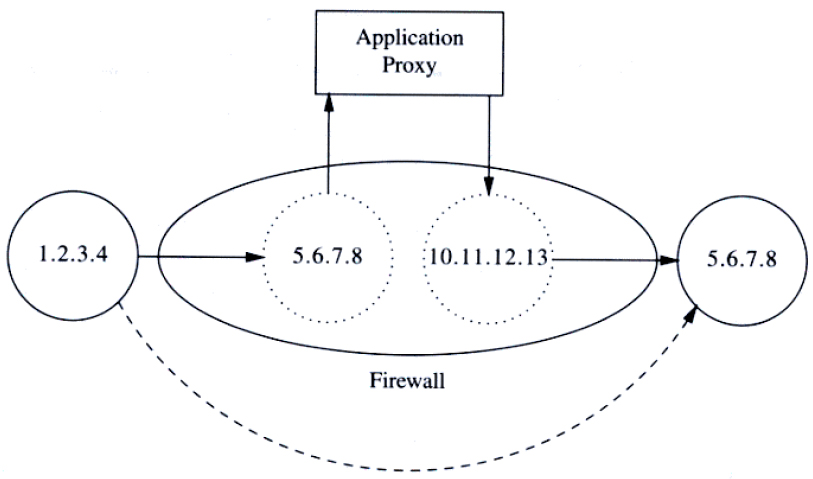
\includegraphics[scale=.5]{fireproxy.jpg}
	\caption{Un filtru dinamic de pachete cu un proxy la nivel aplica'tie. Adresa surs'a este schimbat'a.}
	\label{fireproxy}
\end{figure}

UDP este tratat 'in acela'si mod ca 'si TCP, cu o excep'tie important'a: pentru c'a nu exist'a no'tiunea de terminare a conexiuni 'in UDP, un timeout sau alt'a metod'a euristic'a, cum ar fi num'ararea pachetelor, trebuie folosit'a pentru a 'inchide 'si dealoca obiectele socket create.

Tratarea pachetelor ICMP de eroare este ceva mai complex'a; majoritatea sunt totu'si destul de u'sor de procesat de acest model cu dubl'a conexiune. Dac'a un pachet ICMP sose'ste pentru o anumit'a conexiune, care este u'sor de determinate prin mecanisme uzuale, un pachet corespunz'ator este sintetizat 'si trimis c'atre gazda interioar'a.

Specifica'tia precis'a a comportamentului unu filtru dinamic de pachete este urm'atoarea(c'jnd pachetele vin pe o interfa't'a, urm'atoarele tabele sunt consultate, 'in ordine):

\begin{enumerate}
	\item Tabelul de conexiuni active. Intr'arile din acest tabel pointeaz'a spre o structur'a socket, care, la r'jndul ei, indic'a implicit dac'a datele trebuie copoate 'intr-un socket de ie'sire sau trimise unei aplica'tii proxy.
	\item Un tabel obi'snuit de filtrare, care poate spcifica c'a pachetele sunt permise(sau blocate) f'ar'a a crea o stare local'a. Unele firewall-uri omit acest tabel.
	\item Tabelul dinamic, care for'teaz'a crarea structurilor socket locale. Acest tabel poate avea, de asemenea, intr'ari ``de blocare''.
\end{enumerate}

Dac'a cel de-al doilea tabel nu exist'a, semantica ('si o mare parte din implementare) acestui tip de firewall este identic'a cu cea a unui gateway de circuit sau de aplica'tie.
%4.5.1

%4.5.2
\subsection{Topologie}
Cu tipurile tradi'tionale de firewall-uri, nu conteaz'a dac'a mai mult de un firewall este folosit 'intre o pereche de re'tele. Filtrele de pachete sunt f'ar'a stare; 'in cazul gateway-urilor de nivel circuit sau aplica'tie, clientul deschide o conexiune explicit'a c'atre firewall, astfel 'inc'jt toate conversa'tiile trec prin acela'si punct.

Filtrele dinamice se comport'a diferit. Sunt proiectate astfel 'inc'jt clien'tii s'a nu 'stie de existen'ta lor. Aceste firewall-uri captureaz'a pachetele care sunt rutate spre ele. Dac'a rutele sunt asimetrice, 'si pachetele dinspre 'si spre re'tea trec prin firewall-uri de acest tip diferite, un filtru nu va 'sti conversa'tiile ini'tiate 'si mediate de cel'alalt. Acest lucru va cauza blocarea pachetelor r'aspuns 'si, implicit, e'secul conversa'tiei.

Se pot evita aceste rute asimetrice? Din p'acate nu, 'in unele cazuri vor fi norma, nu excep'tia. 

S'a consider'am topologia re'telei din figura \ref{asymrout}, unde re'teaua exterioar'a este Internetul. 'In general, router-ele de la grani'ta re'telei, conectate la Internet, nu transmit('si nici nu pot) informa'tie de rutare despre topologia 'intregului Internet spre interior; 'in schimb, 'inainteaz'a o rut'a standard. Dac'a cele dou'a filtre dinamice 'inainteaz'a \emph{default}, pachetele destinate spre exterior vor merge c'atre cel mai apropiat punct de ie'sire. 'In acest caz toate pachetele de la gazda $H_1$ vor p'ar'asi re'teaua via $F_1$, 'in timp ce cele de la $H_2$ vor ie'si prin $F_2$.

\begin{figure}[ht]
	\centering
	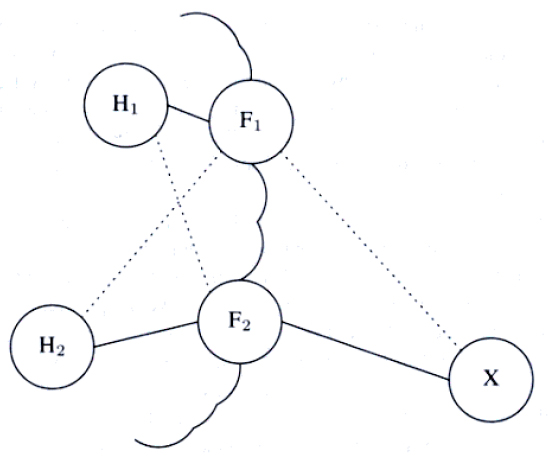
\includegraphics[scale=.6]{asymrout.jpg}
%Usually, the route taken from Host A to Host B is the same as the route used to get back from Host B to Host A; the route is then called symmetric.In complex setups, the route back may be different; in this case, it is asymmetric.
	\caption{Rute asimetrice(drumul de 'intoarcere este diferit de cel de ducere) cu dou'a filtre dinamice de pachete. Liniile punctate indic'a rutele alese; liniile continue indic'a rutele nealese pe baza informa'tiilor de rutare.}
	\label{asymrout}
\end{figure}

Problema const'a 'in faptul c'a lumea exterioar'a nu cunoa'ste nimic despre topologia interioar'a. 'In general, $F_1$ 'si $F_2$ vor ``spune'' am'jndou'a c'a au costuri egale c'atre toate gazdele interioare, a'sa c'a r'aspunsurile vor fi trimise firewall-ului mai apropiat de gazda exterioar'a. A'sadar, dac'a $H_1$ ini'tiaz'a o conexiune c'atre X, pachetele spre exterior vor trece prin $F_1$, 'in timp ce r'aspunsurile vor trece prin $F_2$.

C'jteva posibile solu'tii se v'ad imediat. Prima, desigur, este s'a se re'tin'a informa'tia complet'a despre topologie de amble p'ar'ti ale firewall-ului, pentru a elimina rutele asimetrice. Ceea ce este imposibil din cauza imensit'a'tii Internetului.

Totu'si, informa'tia complet'a despre topologia propriei re'tele este 'in general posibil de acumulat 'in firewall-urile interne. 'In acest caz filtrele dinamice nu mai reprezint'a o problem'a a'sa de mare.

O alt'a strategie const'a 'in partajarea informa'tiei de stare 'intre firewall-uri. Adic'a dac'a o conxiune este f'acut'a prin $F_1$, $F_2$ va fi informat. O alternativ'a ar fi ``\emph{lazy sharing}'': un firewall va 'intreba celelalte firewall-uri 'inainte s'a blocheze un pachet sau s'a 'intrerup'a o conexiune a c'arei stare era partajat'a.

De'si, 'in principiu, aceast'a schem'a ar putea func'tiona, exist'a unele probleme. De exemplu, volumul de mesaje poate fi prohibitiv. Majoritatea conexiunilor TCP constau din schimbul a aporximativ 20 de pachete. Cu c'jt implementarea unui filtru dinamic este mai aproape de modelul ideal, cu at'jt mai mult'a informa'tie de stare trebuie comunicat'a, incluz'jnd update-uri pentru numerele de secven't'a a fiec'arui pachet transmis. Acest lucru este 'si mai evident 'in cazul aplica'tiilor proxy. 'In plus, acest tip de schem'a cere o complexitate 'si mai mare a codului, pentru implementare.

'In majoritatea situa'tiilor, cea mai bun'a solu'tie este folosirea tehnicii cu translatare de adres'a descris'a mai sus. Pachetele spre exterior vor trece prin cel mai apropiat gateway de gazda transmi't'atoare, dar pentru lumea exterioar'a, conexiunea va p'area c'a apar'tine gateway-ului 'insu'si, a'sa c'a pachetele r'aspuns vor fi direc'tionate spre acela'si gateway de fiecare dat'a. Aceast'a schem'a poate fi suboptim'a din punct de vedere al performan'tei, dar este simpl'a 'si eficient'a.

Alternativa const'a 'in instalarea unui singur firewall protejat de un UPS(uninterruptible power supply), deoarece echipamentul ar trebui s'a func'tioneze luni 'intregi f'ar'a reboot-are.
%4.5.2

%4.5.3
\subsection{Siguran't'a}
Filtrele dinamice sunt transparente precum cele statice, dar, spre deosebire de aceste, men'tin starea conexiunilor. Se poate spune c'a securitatea oferit'a de acest tip de firewall-uri este mai bun'a dec'jt cea oferit'a de celelalte tipuri. 

Problema major'a este, ca 'intotdeauna, complexitatea. Dac'a strategia de implementare este destul de simpl'a, ceea ce nu este u'sor de evaluat pentru un produs comercial, atunci siguran'ta oferit'a poate fi comparat'a cu cea a gateway-urilor de nivel circuit.

Mai exist'a un punct ce trebuie luat 'in calcul. Dac'a modelul de securitate include posibilitatea existen'tei unui atacator(sau a unui soft mali'tios) 'in interiorul re'telei, care ar putea 'incerca s'a abuzeze de conexiunea la Internet oferit'a, s-ar putea ca evitarea acestui tip de firewall-uri s'a fie benefic'a. Motivul este transparen'ta; o conexiune TCP oarecare, precum cea creat'a de un vierme, va func'tiona. Un gateway de nivel circuit sau aplica'tie 'si, 'in particular, unul care impune autentificare, este mult mai rezistent acestui tip de amenin't'ari.
%4.5.3
%4.5

%4.6
\section{Firewall-uri distribuite}
O form'a mai nou'a de firewall-uri este reprezentat'a de firewall-urile distribuite. 'In cazul firewall-urilor distribuite, fiecare gazd'a din re'tea va implementa politica de securitate, dar schema acesteia este definit'a de un punct administrativ central. Cu alte cuvinte, prezen'ta unei cutii firewall la marginea re'telei care s'a resping'a orice apel c'atre portul 80, este 'inlocuit'a de un set de reguli care specific'a blocarea portului 80, creat de un administrator 'si apoi distribuit fiec'arei gazde din domeniul de administrare.

Avantajele unei astfel de scheme sunt destule. Unul dintre ele este lipsa unui punct central prin care trec toate pachetele 'si care se poate defecta, lucru ce va afecta toat'a re'teaua. Un altul ar fi abilitatea de a proteja sisteme care nu apar'tin unui spa'tiu izolat. Laptop-urile 'si calculatoarele angajatilor care lucreaz'a acas'a(telecommuters) constituie un astfel de exemplu. 

Exist'a c'jteva produse comerciale care se comport'a 'in acest mod. De asemenea, se poate implementa aceast'a schem'a prin combinarea unui mecanism de nivel 'inalt de specificare a politicii de securitate cu orice mecanism de distribu'tie cum ar fi \emph{rsync} sau \emph{Server Management System(SMS)} de la Microsoft.

Firewall-urile distribuite au o singur'a problem'a major'a. De'si blocarea conexiunilor se poate realiza u'sor, este mult mai greu s'a se permit'a anumite servicii 'in mod selectiv(adic'a doar unele din gazde s'a aib'a acces la acel serviciu). Solu'tia const'a 'in folosirea \emph{IPsec}(o suit'a de protocoale ce au ca scop securizarea protocolului IP prin autentificarea 'si/sau criptarea fiec'arui pachet IP) pentru a identifica colocutorii de 'incredere. Cu alte cuvinte, un sistem este considerat de 'incredere dac'a 'si numai dac'a se poate autentifica criptografic; adresa IP este irelevant'a.
%4.6

%4.7
\section{Firewall-uri personale}
Un firewall personal este o aplica'tie care controleaz'a traficul care pleac'a 'si care vine spre un calculator conectat la o re'tea, permi't'jnd sau nu stabilirea conexiunilor pe baza unei politici de securitate.

Un firewall personal difer'a de un firewall conven'tional 'in ceea ce prive'ste nivelul la care opereaz'a. Aceste aplica'tii sunt proiectate pentru a fi folosite de un utilizator a unei gazde din re'tea(end-user). Ca urmare, un firewall personal nu va proteja dec'jt calculatorul pe care este instalat.

Majoritatea firewall-urilor personale sunt capabile s'a controleze fluxul de informa'tie prin anun'tarea utilizatorului de fiecare dat'a c'jnd se 'incearc'a stabilirea unei conexiuni, 'si prins adaptarea politicii de securitatea pe baza op'tiunii alese de utilizator 'in cazul conexiunii respective. Unele astfel de aplica'tii pot asigura 'si un nivel de detectare a intruziunii, permi't'jnd 'inchiderea unei conexiuni 'in contextul c'areia suspecteaz'a c'a se desf'a'soar'a ac'tiuni intruzive.

Un firewall personal poate oferi o parte din urm'atoarele op'tiuni:

\begin{itemize}
	\item Alertarea utilizatorului 'in leg'atur'a cu 'incerc'arile de conxiune init'iate de aplica'tiile ce ruleaz'a pe sistem;
	\item Oferirea posibilita'tii de a controla ce programe pot accesa re'teaua local'a 'si Internetul 'si ce programe nu pot face acest lucru;
	\item Ascunderea sistemului de scanarea de porturi prin 'impiedicarea r'aspunsurilor la trafic nesolicitat;
	\item Monitorizarea aplica'tiilor care ``asculta'' pe anumite porturi pentru eventuale conexiuni;
	\item Monitorizarea 'intregului trafic Internet(spre sau dinspre);
	\item Prevenirea traficului de re'tea nedorit cauzat de anumite aplica'tii locale;
	\item Oferirea de informa'tii c'atre utilizator despre aplica'tiile care folosesc Internetul;
	\item Oferirea de informa'tii despre serverul destina'tie cu care aplica'tia 'incearc'a s'a comunice.
\end{itemize}

Aceste tipuri de aplica'tii au primit 'si critici. Iat'a c'jteva dintre ele:

\begin{itemize}
	\item Un firewall este un serviciu 'in plus care consum'a resursele sistemului 'si poate, de asemenea, fi 'tinta unui atac;
	\item Dac'a sistemul a fost compromis de un tip malware, acesta poate manipula firewall-ul, ambele rul'jnd pe acela'si sistem; este posibil'a astfel ocolirea mecanismelor de protec'tie oferite de firewall sau chiar 'inchiderea lui;
	\item Astfel de aplica'tii pot genera 'si alarme false, ceea ce poate fi extrem de ``enervant'' pentru utilizator;
	\item Pot interfa'ta cu sistemul de operare 'in \emph{kernel mode} ceea ce poate conduce la instabilitate 'si la apari'tia de bug-uri 'in sistemul de securitate;
\end{itemize}
%4.7

%4.8
\section{Ce nu poate face un firewall}
De'si firewall-urile sunt o parte util'a din programul de securitate al unei re'tele, nu constituie un ``leac'' universal. C'jnd sunt administrare cum se cuvine, sunt folositoare, dar nu pot face fa't'a tuturor pericolelor. Dac'a nu sunt folosite a'sa cum trebuie, singurul lucru pe care 'il asigur'a este o fals'a senza'tie de securitate.

Firewall-urile sunt neputincioase 'imopotriva atacurilor din interior. Un atac din interior poate proveni de la un utilizator ``legitim'' care nu mai coopereaz'a, sau de la cineva care a ob'tinut acces la o gazd'a intern'a prin diverse mijloace. Codul mali'tios care se execut'a pe o ma'sin'a din interior(posibil ajuns acolo via e-mail sau prin exploatarea bug-urilor unor aplica'tii, cum ar fi buffer overflow), poate fi, de asemenea, v'azut ca un atacator interior.

Unele organiza'tii au un model mai strict 'in ceea ce prive'ste atacurile interioare dec'jt altele. Unele b'anci au departamente foarte bine dezoltate care se ocup'a cu a'sa ceva. Aceste organiza'tii care prezint'a riscuri mari de atacuri din interior, 'i'si monitorizeaz'a re'teaua intern'a foarte atent 'si desfiin'teaz'a sistemele suspectate de asa ceva. Organiza'tiile militare prezint'a la r'jndul lor astfel de riscuri. 

Dac'a firewall-ul este singurul sistem de securitate 'si un atacator reu'se'ste s'a ajung'a in interior, situa'tia nu este prea fericit'a. De exemplu, dac'a se face o scanare de viru'si doar la gateway-ul de mail, securitatea poate fi ``spart'a'' dac'a cineva aduce un disc infectat sau download-eaz'a un executabil de pe Web. Orice backdoor care dejoac'a mecanismul de filtrare al gateway-ului este o dovad'a a limitelor eficien'tei unui firewall. Problemele 'in procesarea MIME, cum ar fi buffer overflow, au condus la probleme de securitate care sunt 'in afara scopului unui firewall.

No'tiunea de 'inveli's ``dur'' cu un interior ``moale'' asigur'a securitate dac'a nu exist'a nici un mod de a p'atrunde 'in interior. Ceea ce de obicei este nerealist.

Necooperarea utilizatorilor legitimi este un caz special, dar reprezint'a o problem'a social'a. Marcus Ranum (un cercet'ator 'in domeniul securit'a'tii) a spus: ``Nu po'ti rezolva problemele oamenilor cu software.''. De exemplu, este u'sor pentru indivizi care nu vor s'a coopererze s'a construiasc'a tunele, cum ar fi IP peste HTTP. Filtrarea la nivelul re'tea este neputincioas'a 'in acest caz.

Firewall-urile func'tioneaz'a la un anumit nivel 'in stiva de protocoale, ceea ce 'inseamn'a c'a nu inspecteaz'a datele privite prin prisma nivelelor mai 'inalte. De exemplu, dac'a se face filtrare la nivelul de transport se vor neglija problemele de la nivelul SMTP. Este important'a evaluarea riscurilor la fiecare nivel 'si ac'tionarea pe baza rezultatelor evalu'arilor. Exist'a pre'turi care trebuiesc pl'atite. Filtrarea la nivele 'inalte este intruziv'a, necesit'a mai mult'a putere de procesare, 'si este mai pu'tin evident'a, deoarece exist'a mai multe op'tiuni de procesare pentru fiecare pachet cu c'jt se urc'a 'in stiva de protocoale.

Scanarea de viru'si la gateway-ul da mail reprezint'a un lucru bun pentru siturile pe servere Windows. Dar o strategie mai bun'a este s'a se ruleze un produs antivirus la gateway 'si alt produs la gazde(produsele antivirus nu sunt perfecte). Pe de alt'a parte, 'incercarea de a scana download-urile FTP nu aduce prea multe benficii majorit'a'tii site-urilor. Transformarea datelor, cum ar fi compresia, fac acest lucru practic imposibil. 

A decide unde se va face filtrarea 'si ``c'jt de mult'' este o chestiune de balans 'intre risc 'si cost. Exist'a 'intotdeauna un nivel mai 'inalt, incluz'jnd persoanele care urmeaz'a instruc'tiuni stupide primite prin mail. Nu e prea u'sor s'a se filtreze a'sa ceva.

O alt'a problem'a a firewall-urilor este 'increderea tranzitiv'a. Dac'a A are 'incredere 'in B prin firewall, 'si B are 'incredere 'in C, atunci A va avea 'incredere 'in C, ``chiar dac'a vrea sau nu''(chiar dac'a se 'stie acest lucru sau nu).

Pe l'jng'a toate acestea, firewall-urile pot avea erori sau pot func'tiona cum nu ar trebui. Cea mai bun'a administra'tie nu poate face nimic 'impotriva unui firewall care nu opereaz'a a'sa cum este specificat c'a trebuie s'a opereze.
%4.8
%CapIV Ziduri de foc

%CapV Aplicatie
\chapter{Aplica'tie}
Aplica'tia pe care am dezvoltat-o este un firewall personal sub sistemul de operare Microsoft Windows XP. Scopul acestei aplica'tii este de a permite unui utilizator s'a controleze traficul de informa'tie spre 'si dinspre Internet. Exist'a doua moduri prin care aplica'tia 'indepline'ste acest scop. Primul permite utilizatorului s'a specifice reguli de filtare pe baza adreselor IP 'si porturilor con'tinute 'in antetele pachetelor IP. Cel de-al doilea mod const'a in monitorizarea aplica'tiilor care ruleaz'a la nivel de utilizator 'si care folosesc interfa'ta \emph{Winsock} a sistemului de operare pentru a transmite 'si a primi date de pe Internet. Numele programului este ``\emph{NetProtector}''.

%5.1
\section*{Func'tionare}
Dup'a cum am spus mai sus, aplica'tia con'tine dou'a module care 'indeplinesc anumite sarcini. Cel de-al treilea modul, interfa'ta cu utilizatorul(GUI), este punctul central de unde sunt coordonate celelalte dou'a. GUI-ul permite utilizatorului s'a specifice reguli de filtrare pe care apoi le transmite primului modul. De asemenea, permite celui de-al doilea modul 'ins'arcinat cu monitorizarea aplica'tiilor s'a 'in'stiin'teze utilizatorul atunci c'jnd o aplica'tie 'incearc'a sa se conecteze la Internet sau c'jnd ``ascult'a'' pe un anumit port.
%5.1

%5.2
\section*{Mecanisme folosite}
Aplica'tia este dezvoltat'a 'in limbajul C++ folosind mediul de dezoltare Visual Studio 2008. Modulul grafic este construit cu ajutorul MFC(Microsoft Foundation Classes). Aceasta este o bibliotec'a de tip ``wrapper'' care 'impacheteaz'a por'tiuni din Windows API 'in clase C++ pentru a facilita anumite opera'tiuni 'si pentru a oferi un model orientat-obiect. 

Modulul 'ins'arcinat cu filtrarea pachetelor este un dirver care func'tioneaz'a in mod nucleu, 'si este dezvoltat folosind WDK(Windows Driver Kit). WDK este un set de unelte de la Microsoft care permite construirea driver-elor de sistem pentru platforma Microsoft Windows. Deoarece Visual Studio nu are suport pentru compilarea acestui tip de module, am folosit un program numit \emph{DDKWizard}(disponibil la \url{http://ddkwizard.assarbad.net/}) care adaug'a acest suport prin folosirea c'jtorva ``trucuri''.

Modulul care monitorizeaz'a aplica'tiile este, de fapt, un DLL(Dynamic-link library) ce va fi 'inc'arcat 'in memorie de interfa'ta Winsock pentru ficare aplica'tie care o 'intrebuin'teaz'a. Este posibil'a astfel interceptarea oric'arei opera'tii de conectare la internet 'ini'tiat'a de orice aplica'tie care folo'sete Winsock (majoritatea fac acest lucru) 'si raportarea acestei 'incerc'ari programului propriu-zis (modulul grafic central).

%5.2.1
\subsection*{Filter-Hook Driver}
'In Windows 2000 DDK(driver development kit, precursorul WDK) Microsoft include un nou tip de driver numit Filter-Hook Driver. Prin intermediul acestui modul se poate 'inregistra o func'tie care s'a filtreze tot traficul care sose'ste sau pleac'a de la interfe'tele sistemului(un calculator poate avea mai multe pl'aci de re'tea). Acest driver nu e un driver de re'tea propriu-zis, ci este un driver de mod kernel ce poate fi folosit la extinderea func'tionalit'a'tii driver-ului \emph{IP Filter Driver}. Practic, 'in modulul Filter-Hook Driver se implementeaz'a o func'tie de tip ``callback'' care apoi se 'inregistreaz'a prin intermediul IP Filter Driver. 'In acest moment IP Filter Driver va apela func'tia 'inregistrat'a de fiecare dat'a c'jnd un pachet este primit sau trimis(unul din parametrii func'tiei este un pointer c'atre loca'tia de memorie unde este stocat pachetul).

Aceasta nu este unica metod'a prin care se pot contrui firewall-uri pentru Windows. Iat'a principalele metode de implementare a unui firewall:

\begin{itemize}
	\item Mod utilizator:
		\begin{itemize}
			\item \emph{Winsock Layered Service Provider (LSP)} - metoda folosit'a de cel de-al doilea modul pentru a avea acces la nivelul aplica'tie;
			\item \emph{Windows 2000 Packet Filtering Interface} - permite aplica'tiilor user-mode s'a specifice reguli care sunt folosite de componente TCP/IP de nivel jos pentru a filtra pachetele;
			\item \emph{Winsock Replacement DLL} - o modalitate folosit'a 'inaite s'a apar'a Winsock Layered Service Provider.
		\end{itemize}
	\item Mod nucleu:
		\begin{itemize}
			\item \emph{Transport Data Interface (TDI) Filter Driver} - un driver filtru situat peste modulul TCP/IP;
			\item \emph{NDIS Intermediate (IM) Driver} - NDIS vine de la ``Network Driver Interface Specification'';
			\item \emph{Windows 2000 Filter-Hook Driver}
			\item \emph{Windows 2000 Firewall-Hook Driver}
			\item \emph{NDIS-Hooking Filter Driver} - cel mai jos nivel 'in stiva de protocoale.
		\end{itemize}
\end{itemize}

Principalele avantaje oferite de Filter-Hook Driver sunt:

\begin{enumerate}
	\item Asigur'a flexibilitate filtr'arii; se poate filtra tot traficul la nivel IP(sau peste acest nivel);
	\item Este o metod'a u'sor de implementat(fa't'a de celelalte)
\end{enumerate}

Aceast'a modalitate prezint'a 'si o serie de dezavantaje: nu se pot filtra cadrele de sub IP(de exemplu cadrele Ethernet, este nevoie de un filtru la nivel NDIS pentru acest lucru) 'si numai o singur'a func'tie poate fi 'inregistrat'a la un momentdat. Ultimul este motivul pentru care nu este folosit de produsele firewall comerciale(dac'a o alt'a aplica'tie a 'inregistrat deja o astfel de func'tie, restul programelor nu mai pot face acest lucru).

Filter-Hook Driver nu reprezint'a cea mai bun'a metod'a de implementare a unui firewall, dar poate fi un bun 'inceput pentru cei interesa'ti de acest domeniu.
%5.2.1

%5.2.2

\begin{figure}[ht]
	\centering
	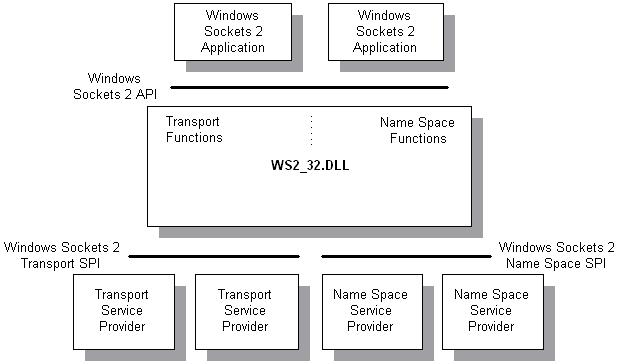
\includegraphics[scale=.5]{spi.jpg}
	\caption{Arhitectura Winsock 2}
	\label{spi}
\end{figure}

\subsection*{Layered Service Provider}
Una din op'tiunile interesante pe care Winsock 2 le ofer'a este a'sa-numita ``service provider interface'' sau SPI. Aceast'a interfa't'a este implementat'a de provider-ii de servicii de transport care se afl'a a'seza'ti sub modulul Winsock(arhitectura Winsock 2 se poate observa 'in figura \ref{spi}). Func'tionalitatea unui provider de servicii de transport poate fi extins'a prin implementarea unui modul LSP(Layered Service Provider) 'si a'sezarea acestuia peste sau 'intre celelalte module care alc'atuiesc provider-ul. De exemplu la acest nivel poate fi implementat QOS(Quality of Service) sau, ca 'in cazul de fa't'a, un ``mic'' firewall. S'a observ'am c'a este un loc perfect 'si pentru programele mali'tioase(pot fi capturate informa'tii 'si retransmise apoi c'atre un eventual atacator).

Practic, acest modul este o libr'arie dinamic'a(DLL), iar pentru 'inregistrarea 'si pozi'tionarea lui 'in cataogul Winsock, sunt puse la dispozi'tie cateva func'tii ce pot fi apelate de o aplica'tie normal'a user-mode.

Exist'a 'itotdeauna un provider de baz'a(care este responsabil cu setarea conexiunilor 'si transferul datelor) peste care se pot stivui module LSP care implementeaz'a divese func'tionalit'a'ti de nivel mai 'inalt. Lucrul pe care 'il au 'in comun este c'a trebuie s'a implementeze o anumit'a interfa't'a (figura \ref{spi2}).

\begin{figure}[ht]
	\centering
	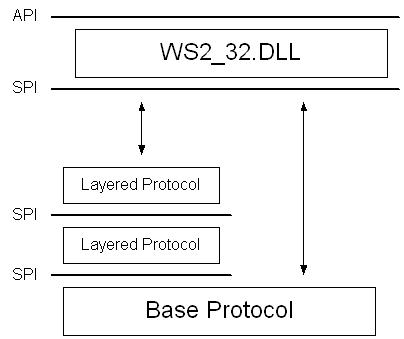
\includegraphics[scale=.5]{spi2.jpg}
	\caption{Protocoalele}
	\label{spi2}
\end{figure}
%5.2.2

%5.3
\section*{Implementarea modulelor}
\paragraph{Modulul Filter-Hook Driver} pe l'jng'a func'tia descris'a mai sus, implementeaz'a patru opera'tii pe care le pune la dispozi'tie aplica'tiei propriu-zise. Aceste sunt: start('inregistrarea func'tiei ``c'jrlig''), stop(retragerea acestei func'tii), ad'augarea unei reguli 'si 'stergerea unei reguli. Regulile sunt ni'ste structuri ce con'tin un identificator pentru un circuit(adic'a adres'a surs'a, adres'a destina'tie, port surs'a 'si port destina'tie) pe baza c'arora se face filtrarea. Aceste structuri sunt 'tinute 'intr-o list'a simplu 'inl'an'tuit'a care este parcurs'a de func'tia de filtrare de fiecare dat'a c'jnd este apelat'a. Dac'a pachetul corespunde vruneia dintre regulile din list'a, acesta este blocat. A'sadar politica de filtrare este: ``tot cea ce nu este specificat 'in reguli, este permis''.

\paragraph{Modulul LSP} este proiectat pornind de la un exemplu pus la dispozi'tie de Microsoft. Practic, sunt modificate doar func'tiile de conectare(WSPConnect) 'si de ascultare pe un anumit port(WSPListen). 'In aceste func'tii un mesaj blocant este transmis aplica'tiei propriu-zise, 'inainte de a se apela rutina implementat'a de modulul situat sub acest LSP. Acest mesaj con'tine num'arul de identificare al procesului curent(PID; segmentul de date al DLL-ului este 'inc'arcat o singur'a dat'a 'in memorie dar c'jnd este folosit de un proces va func'tiona 'in contextul procesului respectiv, a'sadar va transmite PID-ul corect). Se a'steapt'a apoi r'aspunsul de la aplica'tia principal'a.

\paragraph{NetProtector} este programul principal care alc'atuie'ste acest firewall. Acesta afi'seaz'a o fereastr'a care asigur'a o interfa't'a ``prietenoas'a'' ce permite utilizatorului s'a controleze cele dou'a module despre care am vorbit mai sus. La pornire, aplica'tia 'incarc'a modulul Filter-Hook Driver 'si 'il porne'ste. Regulile pe care utilizatorul le specific'a sunt salvate 'in Windows Registry 'si la fiecare pornire sunt transmise modulului de filtrare dup'a 'inc'arcarea acestuia. Programul implementeaz'a o func'tie handler pentru mesajul primit de la modulul LSP. 'In aceast'a func'tie, dac'a exist'a o regul'a impus'a deja pentru procesul de la care a fost primit mesajul, atunci la mesaj se va r'aspunde conform regulii respective(accesul va fi blocat sau permis). Dac'a nu exist'a o astfel de regul'a, NetProtector va notifica utilizatorul de conexiunea ce este pe cale sa fie stabilit'a(sau de faptul c'a un proces a'steapt'a o conexiune) 'si va a'stepta ca acesta s'a specifice cum va fi tratat'a conexiunea('si dac'a toate conexiunile acelui program trebuie tratate la fel).
%5.3

%5.2

%CapV Aplicatie

%CapVI Concluzii
\chapter{Concluzie}
'In 'incheierea acestei lucr'ari voi prezenta un citat care apar'tine lui Bruce Schneier, un expert 'in domeniul securit'a'tii informatice:

\begin{quote}
'In r'azboi informa'tia este putere. Cu c'jt 'i'ti 'intelegi mai bine inamicul, cu at'jt vei fi mai capabil s'a 'il infr'jngi. 'In r'azboiul 'impotriva hacker-ilor du'sm'ano'si, a celor care ``sparg'' re'tele, 'si a altor ``p'al'arii negre'' din ciber-spa'tiu, cei de partea ``binelui'' au surprinz'ator de pu'tine informa'tii. Cei mai mul'ti profesioni'sti din securitate, chiar 'si cei care proiecteaz'a scule de securitate, ignor'a uneltele, tacticile 'si motiva'tiile inamicilor. 'Si aceast'a stare este favorabil'a inamicilor.
\end{quote}

Ceea ce este trist 'in toat'a aceast'a poveste este faptul c'a dup'a at'j'tia ani, comunit'a'tile programatorilor, proiectan'tilor de sisteme 'si administratorilor nu au 'inv'a'tat lec'tia cu privire la securitatea informatic'a. Acelea'si tehnici de atac folosite acum c'j'tiva ani sunt valabile 'si 'in prezent. Dac'a, 'intr-adev'ar, o schimbarea 'in arhitectura Internetului, de'si ar putea rezolva multe probleme de securitate, este imposibil de efectuat, cel pu'tin implement'arile unor programe 'si noile protocoale care apar pot fi construite f'ar'a s'a se neglijeze securitatea.

Exist'a diferite tipuri de mijloace de protec'tie, 'si destui produc'atori pe pia't'a, dar 'intotdeauna este mai eficient, 'si de obicei mai simplu, s'a previi o problem'a dec'jt s'a o comba'ti. De'si mai mul'ti speciali'sti 'in securitate au propus diferite solu'tii cu privire la securitatea Internetului, acestea implic'a, de cele mai multe ori, modific'ari de infrastructur'a, modific'ari ce nu pot fi efectualte pe scar'a larg'a at'jt de u'sor.

'In final, a's dori s'a subliniez 'inc'a o dat'a importan'ta securit'a'tii informa'tiei 'si in special a securit'a'tii pe Internet, amintind c'a sistemul care ne aduce ast'azi at'jtea avantaje, are destule puncte slabe, iar dac'a dorim s'a beneficiem 'in continuare de aceste avantaje, f'ar'a s'a ne temem de diverse pericole, trebuie s'a administr'am Internetul cu grij'a, nefiind ignoran'ti 'in ceea ce prive'ste securitatea.
%CapVI Concluzii

%bibliografie

%bibliografie:
%William R. Cheswick, Steven M. Bellovin, Aviel D. Rubin - Firewalls and Internet Security Second Edition: Repelling the Willy Hacker

%W. Richard Stevens - TCP/IP Ilustrated
%http://en.wikipedia.org/wiki/Rpc
%http://www.rhyshaden.com/rpc.htm
%http://en.wikipedia.org/wiki/Www
%http://www.tcpipguide.com/free/t_TelnetProtocol.htm
%http://en.wikipedia.org/wiki/Network_Time_Protocol

%http://www.ranum.com/security/computer_security/archives/internet-attacks.pdf
%http://en.wikipedia.org/wiki/Social_engineering_(security)
%http://en.wikipedia.org/wiki/Exploit_(computer_security)
%http://en.wikipedia.org/wiki/Malware
%http://www.isc.org/index.pl?/ops/ds/host-count-history.php
%http://en.wikipedia.org/wiki/Denial-of-service_attack
%http://www.cs.cmu.edu/~mihaib/articole/tcp/tcp-html.html
%http://www.cs.washington.edu/homes/savage/papers/CCR99.ps
%http://en.wikipedia.org/wiki/E-mail_spoofing
%http://en.wikipedia.org/wiki/Website_spoofing
%http://en.wikipedia.org/wiki/Cross-site_scripting
%http://www.linux-magazin.ro/pdf/ 04/lm_04_dec_03_091-093_crosssite.pdf
%http://www.cs.cmu.edu/~mihaib/articole/ddos/ddos-html.html
%http://en.wikipedia.org/wiki/Computer_virus
%http://en.wikipedia.org/wiki/Timeline_of_notable_computer_viruses_and_worms
%http://en.wikipedia.org/wiki/Computer_worm
%http://www.cs.cmu.edu/~mihaib/articole/codered/codered-html.html
%http://www.caida.org/research/security/code-red/coderedv2_analysis.xml

%http://en.wikipedia.org/wiki/Personal_firewall

\begin{thebibliography}{9}
	\bibitem{Cheswick03}William R. Cheswick, Steven M. Bellovin, Aviel D. Rubin, 2003. \emph{Firewalls and Internet Security: Repelling the Wily Hacker, Second Edition}
	\bibitem{stevens94} W. Richard Stevens, 1994. \emph{TCP/IP Illustrated, Volume 1: The Protocols}
	\bibitem{wikirpc} \url{http://en.wikipedia.org/wiki/Rpc}
	\bibitem{diagrpc} \url{http://www.rhyshaden.com/rpc.htm}
	\bibitem{wikitelnet} \url{http://www.tcpipguide.com/free/t_TelnetProtocol.htm}
	\bibitem{wikiwww} \url{http://en.wikipedia.org/wiki/Www}
	\bibitem{diagntp} \url{http://en.wikipedia.org/wiki/Network_Time_Protocol}
	\bibitem{wikiattacks} \url{http://www.ranum.com/security/computer_security/archives/internet-attacks.pdf}
	\bibitem{wikisoceng} \url{http://en.wikipedia.org/wiki/Social_engineering_(security)}
	\bibitem{wikiexoloit} \url{http://en.wikipedia.org/wiki/Exploit_(computer_security)}
	\bibitem{wikimalware} \url{http://en.wikipedia.org/wiki/Malware}
	\bibitem{wikihostcnt} \url{http://www.isc.org/index.pl?/ops/ds/host-count-history.php}
	\bibitem{wikidos} \url{http://en.wikipedia.org/wiki/Denial-of-service_attack}
	\bibitem{artcolconc} \url{http://www.cs.cmu.edu/~mihaib/articole/tcp/tcp-html.html}
	\bibitem{artcolconc1} \url{http://www.cs.washington.edu/homes/savage/papers/CCR99.ps}
	\bibitem{wikimailspoof} \url{http://en.wikipedia.org/wiki/E-mail_spoofing}
	\bibitem{wikiwebspoof} \url{http://en.wikipedia.org/wiki/Website_spoofing}
	\bibitem{wikixss} \url{http://en.wikipedia.org/wiki/Cross-site_scripting}
	\bibitem{artxss} \url{http://www.linux-magazin.ro/pdf/ 04/lm_04_dec_03_091-093_crosssite.pdf}
	\bibitem{artddos} \url{http://www.cs.cmu.edu/~mihaib/articole/ddos/ddos-html.html}
	\bibitem{wikivirus} \url{http://en.wikipedia.org/wiki/Computer_virus}
	\bibitem{wikivirhist} \url{http://en.wikipedia.org/wiki/Timeline_of_notable_computer_viruses_and_worms}
	\bibitem{wikiworm} \url{http://en.wikipedia.org/wiki/Computer_worm}
	\bibitem{artcodered} \url{http://www.cs.cmu.edu/~mihaib/articole/codered/codered-html.html}
	\bibitem{diagcodered} \url{http://www.caida.org/research/security/code-red/coderedv2_analysis.xml}
	\bibitem{persfire} \url{http://en.wikipedia.org/wiki/Personal_firewall}
	\bibitem{ndis} \url{http://www.ndis.com/papers/winpktfilter.htm}
	\bibitem{lsp} \url{http://www.microsoft.com/msj/0599/LayeredService/LayeredService.aspx}
	\bibitem{filterhook} \url{http://www.codeproject.com/KB/IP/drvfltip.aspx}
\end{thebibliography}
%bibliografie

\end{document}
%DOCUMENTUL PROPRIU-ZIS